%\documentclass[10pt, twocolumn, nocopyrightspace]{sigplanconf}
\documentclass[letterpaper,twocolumn,10pt]{article}
\usepackage{usenix,epsfig,endnotes}

\pdfpagewidth=8.5in
\pdfpageheight=11in

\usepackage{balance}

% comment out the following line when submitting
%\def \oscardebug{}
%\def \oscardraft{}

% rubber: paper letter

% $Id$
\setlength{\paperheight}{11in}

% natbib package in sigplanconf class file conflicts with cite package
\usepackage{paralist}
\usepackage{times}
\usepackage{graphicx}
\usepackage{rotating}
\usepackage{multirow}
\usepackage{listings}
\lstset{language=C}
\usepackage[hyphens]{url}
\usepackage{comment}
\usepackage{color}
\usepackage{xcolor}
\usepackage{array}
\usepackage{booktabs}
\usepackage[sort]{natbib}
\usepackage{paralist}
\usepackage[hidelinks]{hyperref}
\usepackage{titlesec}
\usepackage{titling}

\renewcommand{\ttdefault}{cmtt}

\begin{document}

%% disable hyperref draft mode for submission

% No copyright block for submission
%\makeatletter
%\let\@copyrightspace\relax5
%\makeatother

%\setlength{\columnsep}{.33in}

% Use the following at camera-ready time to suppress page numbers.
% Comment it out when you first submit the paper for review.
\ifx \oscardraft \undefined
\pagestyle{empty}
\makeatletter
  \let\ps@plain\ps@empty
\makeatother
\fi

%\pagenumbering{arabic}

%\singlespace
%% To make table entries readable
\newcommand\T{\rule{0pt}{2.0ex}}
\newcommand\B{\rule[-0.9ex]{0pt}{0pt}}

% Squeeze space
%\renewcommand{\baselinestretch}{0.99}
%\addtolength{\belowcaptionskip}{-10pt}
%\addtolength{\abovecaptionskip}{-5pt}
%\newcommand{\tabpar}[2]{
%    \begin{center} \begin{tabular}{#1} #2 \end{tabular} \end{center}}

%% \newcommand{\by}[2]{\mbox{#1$\times$#2}}

%% \newcommand{\wunits}[2]{\mbox{#1\,#2}}
%% \newcommand{\um}{\mbox{$\mu$m}}
%% \newcommand{\xum}[1]{\wunits{#1}{\um}}
%% \newcommand{\xnm}[1]{\wunits{#1}{nm}}
%% \newcommand{\sig}[1]{${\tt #1}$}
%% \newcommand{\sigb}[1]{$\overline{{\tt #1}}$}

% Make list indentation tight\
\setdefaultleftmargin{1em}{0em}{}{}{}{}

\ifx \oscardebug \undefined
\newcommand{\fixme}[1]{{}}
\newcommand{\fixmedp}[1]{{}}
\else
\newcommand{\fixme}[1]{{\bf\textcolor{red}{ [ FIXME Ts: #1 ]}}}
\newcommand{\fixmedp}[1]{{\bf\textcolor{red}{ [ FIXME dP: #1 ]}}}
\fi

\ifx \oscardebug \undefined
\newcommand{\note}[1]{{}}
\else
\newcommand{\note}[1]{{\bf\textcolor{blue}{ [ NOTE: #1 ]}}}
\fi

\ifx \oscardraft \undefined
\newcommand{\edit}[1]{{#1}}
\newenvironment{edits}{}{}
\else
\newcommand{\edit}[1]{{\textcolor{blue}{#1}}}
\newenvironment{edits}{\color{blue}}{\color{black}}
\fi

% MW adding. To compile without the red, either:
% (1) comment in the following line:
%\def\noeditingmarks{} % or
% (2) compile with a line like:
%    $ latex '\def\noeditingmarks{} \input osdi08
% Also, might be easier to convert your macros to this format. (I like
% having the comments in another color and also being able to turn them
% all off with one command.)
\begin{comment}
\newcommand{\textred}[1]{\textcolor{red}{#1}}
\ifx\noeditingmarks\undefined
    \newcommand{\pgwrapper}[2]{\textred{#1: #2}}
\else
    \newcommand{\pgwrapper}[2]{}
\fi
\newcommand{\mw}[1]{\pgwrapper{MW}{#1}}
\end{comment}

\newcommand{\intel}{Intel}
\newcommand{\sgx}{SGX}
\newcommand{\sdk}{Intel SDK}
\newcommand{\libos}{library OS}
\newcommand{\libc}{libc}
\newcommand{\sysname}{Graphene-SGX}
\newcommand{\graphene}{Graphene}
\newcommand{\haven}{Haven}
\newcommand{\drawbridge}{Drawbridge}
\newcommand{\scone}{SCONE}
\newcommand{\panoply}{Panoply}

\newcommand{\enclavecallnum}{28}
\newcommand{\palcallnum}{36}
\newcommand{\shieldsyscallnum}{145}

\newcommand{\funcname}[1]{{\tt #1}}
\newcommand{\syscall}[1]{{\tt #1}}

\newcommand{\roughly}{$\sim$}

%%%%%%%%%%%%%%SPACING HACKS%%%%%%%%%%%%%%%

% get the top of the title to exactly 1inch from the top of page
\setlength{\droptitle}{-.55in}     % Eliminate the default vertical space
%%\addtolength{\droptitle}{-4pt}   % Only a guess. Use this for adjustment

% reduce the spacing before \paragraph{} commands: (tweak the number before \@plus)
%% \makeatletter
%% \renewcommand{\paragraph}{%
%%   \@startsection{paragraph}{4}%
%%   {\z@}{0.5ex \@plus 1ex \@minus .2ex}{-1em}%
%%   {\normalfont\normalsize\bfseries}%
%% }
%% \makeatother

%% Eliminate widows and orphans if needed 

% reduce the penalties for page breaks in middle of paragraphs
%% \clubpenalty=10
%% \widowpenalty=10
%% \interlinepenalty=10 %hyphens
%% \brokenpenalty=10    %hyphens

%% \def\topfraction{0.9}
%% \def\bottomfraction{0.9}
%% \def\textfraction{0.1}


% minimize spacing between paragraphs
%% \setlength{\parskip}{0pt}
%% \setlength{\parsep}{0pt}
%% \setlength{\headsep}{0pt}
%\setlength{\topskip}{0pt}
%\setlength{\topmargin}{0pt}
%\setlength{\topsep}{0pt}
%\setlength{\partopsep}{0pt}

%% \addtolength{\voffset}{.3125in}
%% \addtolength{\textheight}{-.0625in}
%% \addtolength{\textwidth}{-.0625in}

%\def\name#1{#1}%
%\def\defname#1#2{\expandafter\def\csname #1\endcsname{\name{#2}}\ignorespaces}%
%\thispagestyle{empty}
%% compress the space between title and authorlist
%\numberofauthors{1}
%\authorinfo{names}{Stony Brook}{emails}
%\author{Anonymous submission to SOSP 2013, please do not distribute. Paper \#162, \pageref*{LastPage} pages total.}
%\author{Anonymous submission to EuroSys 2013, please do not distribute.}

%\titlebanner{Draft, please do not distribute}        % These are ignored unless
%\preprintfooter{Draft, please do not distribute}   % 'preprint' option specified.

\def\longconferencenames{}
% Conference macros
% include this in enclosing document for long conference names
%\def\longconferencenames{}

%  Use this one for the cv notes
%\def\includecvnotes{}
%\def\includebionotes{}

\newcommand{\conferencename}[3]{
\ifx\longconferencenames\undefined
\newcommand{#1}[0]{{#2}}
\else
\newcommand{#1}[0]{{#3}}
\fi
}

\newcommand{\cvnote}[1]{
\ifx\includecvnotes\undefined
%
\else
{#1}%
\fi
}


\newcommand{\bionote}[1]{
\ifx\includebionotes\undefined
%
\else
{#1}%
\fi
}


\conferencename{\podc}{PODC}{Proceedings of the ACM symposium on Principles of
distributed computing (PODC)}

\conferencename{\asplos}{ASPLOS}{{Proceedings of the ACM International Conference on Architectural Support for Programming Languages and Operating Systems (ASPLOS)}}

\conferencename{\spaa}{SPAA}{{Proceedings of the ACM symposium on Parallelism in algorithms and architectures (SPAA)}}

\conferencename{\osdi}{OSDI}{{Proceedings of the USENIX Symposium on Operating Systems Design and Implementation (OSDI)}}

\conferencename{\disc}{DISC}{{Proceedings of the International Conference on Distributed Computing (DISC)}}

\conferencename{\usenixatc}{USENIX ATC}{{Proceedings of the USENIX Annual Technical Conference}}
\conferencename{\usenixsec}{USENIX Security}{{Proceedings of the USENIX Security Symposium}}

\conferencename{\pldi}{PLDI}{{Proceedings of the ACM SIGPLAN conference on Programming language design and implementation (PLDI)}}

\conferencename{\computer}{Computer}{{IEEE Computer}}

\conferencename{\sosp}{SOSP}{{Proceedings of the ACM SIGOPS Symposium on Operating Systems Principles (SOSP)}}

\conferencename{\isca}{ISCA}{{Proceedings of the ACM IEEE International Symposium on Computer Architecture (ISCA)}}

\conferencename{\csaw}{CSAW}{{Proceedings of the ACM Workshop on Computer Security Architecture (CSAW)}}

\conferencename{\wddd}{WDDD}{{Proceedings of the Workshop on Duplicating, Deconstructing, and Debunking (WDDD)}}

\conferencename{\vldb}{VLDB}{{Proceedings of the International Conference on Very Large Databases (VLDB)}}

\conferencename{\toplas}{TOPLAS}{{ACM Transactions on Programming Languages and Systems (TOPLAS)}}

\conferencename{\tocs}{TOCS}{{ACM Transactions on Computer Systems (TOCS)}}

\conferencename{\ppopp}{{PPoPP}}{{Proceedings of the ACM SIGPLAN Symposium on Principles and Practice of Parallel Programming (PPoPP)}}

\conferencename{\jpdc}{J. Parallel Distrib. Comput.}{{Journal of Parallel and Distributed Computing}}

\conferencename{\ismm}{ISMM}{{Proceedings of the ACM International Symposium on Memory Management (ISMM)}}

\conferencename{\cacm}{CACM}{{Communications of the ACM (CACM)}}

\conferencename{\hpca}{HPCA}{{Proceedings of the IEEE International Symposium on High-Performance Computer Architecture (HPCA)}}

\conferencename{\transact}{TRANSACT}{{Proceedings of the ACM SIGPLAN Workshop on Transactional Computing (TRANSACT)}}

\conferencename{\iiswc}{IISWC}{{Proceedings of the IEEE International Symposium on Workload Characterization (IISWC)}}

\conferencename{\tpds}{IEEE Trans, Parallel Distrib. Syst.}{{IEEE Transactions on Parallel and Distributed Systems}}

\conferencename{\osr}{OSR}{{ACM Operating Systems Review}}

\conferencename{\nsdi}{NSDI}{{Proceedings of the USENIX Symposium on Networked Systems Design and Implementation (NSDI)}}

\conferencename{\cc}{CC}{{Proceedings of the International Conference on Compiler Construction (CC)}}

\conferencename{\surveys}{ACM Comput. Surv.}{{ACM Computing Surveys}}
\conferencename{\icde}{ICDE}{{Proceedings of the IEEE International Conference on Data Engineering (ICDE)}}
\conferencename{\fast}{FAST}{{Proceedings of the USENIX Conference on File and Storage Technologies (FAST)}}
\conferencename{\eurosys}{{E}uro{S}ys}{{Proceedings of the ACM European Conference on Computer Systems ({E}uro{S}ys)}}
\conferencename{\hotos}{HotOS}{{Proceedings of the USENIX Workshop on Hot Topics in Operating Systems (HotOS)}}
\conferencename{\hotcloud}{HotCloud}{{Proceedings of the USENIX Workshop on Hot Topics in Cloud Computing (HotCloud)}}
\conferencename{\oopsla}{OOPSLA}{{Proceedings of the ACM SIGPLAN Conference on Object-Oriented Programming, Systems, Languages, and Applications (OOPSLA)}}
\conferencename{\ndss}{NDSS}{{Proceedings of the Network and Distributed System Security Symposium (NDSS)}}
\conferencename{\oakland}{IEEE S\&P}{{Proceedings of the IEEE Symposium on Security and Privacy (Oakland)}}
\conferencename{\ispass}{ISPASS}{Proceedings of the IEEE International Symposium on Performance Analysis of Systems and Software (ISPASS)}

\conferencename{\europar}{{E}uro{P}ar}{{Proceedings of the European Conference on Parallel Programming ({E}uro{P}ar)}}

\conferencename{\sigcse}{{SIGCSE}}{{Proceedings of the ACM SIGCSE technical symposium on Computer science education (SIGCSE)}}

\conferencename{\ccs}{{CCS}}{{Proceedings of the ACM Conference on Computer and Communications Security (CCS)}}

\conferencename{\veeconf}{{VEE}}{{Proceedings of the International Conference on Virtual Execution Environments (VEE)}}

\conferencename{\lisa}{{LISA}}{{Proceedings of the Large Installation System Administration Conference (LISA)}}
\conferencename{\scool}{SCOOL}{{Proceedings of the Workshop on Synchronization and Concurrency in Object-Oriented Languages (SCOOL)}}
\conferencename{\cgo}{CGO}{{Proceedings of the International Symposium on Code Generation and Optimization (CGO)}}
\conferencename{\dsn}{{DSN}}{Proceedings of the International Conference on Dependable Systems and Networks (DSN)}
\conferencename{\sac}{{SAC}}{{Proceedings of the ACM Symposium on Applied Computing (SAC)}}

\conferencename{\cluster}{{IEEE Cluster}}{{IEEE International Conference on Cluster Computing}}


%% DP: Note there is a hack in sig-alternate class file to squeeze space under the title for submission.
%\title{Graphene for Shielding: Decentralizing Hardware-Assisted Isolated Execution for Multi-Process Applications}
%\title{Shielding Unmodified Linux Multi-Process Applications with a Multi-Enclave Library OS using Intel SGX}
%\title{Isolating Legacy Applications in Multi-Enclave Environment Using \sysname{} Library OS}
%\title{Shelter the Civilians---Securing Linux COTS Applications with Intel SGX}
\title{Graphene-SGX: A Practical Library OS for Unmodified Applications on SGX}

%\author{Anonymous submission to Security\&Privacy 2017, please do not distribute.}
\author{
{\rm Chia-Che Tsai}\\
Stony Brook University
\and
{\rm Donald E. Porter}\\
University of North Carolina at Chapel Hill \\ and Fortanix
\and
{\rm Mona Vij}\\
Intel Corporation
} % end author

%\vspace{-20pt}}
\date{\vspace{-4ex}} %% compress the space between authorlist and text
%\date{}

\newcommand{\subtitle}[1]{%
  \posttitle{%
    \par\end{center}
    \begin{center}\large#1\end{center}
    \vskip0.5em}%
}

%\subtitle{\bf Draft \today: Please do not distribute}

\maketitle



\titleformat{\section}[block]{
  \fontsize{12}{15}\bfseries}{%
  \thesection}{%
  1em}{%
  }{%
  }%
  
\titlespacing*{\section}
{0pt}{1.5ex plus .1ex}{1ex plus .1ex}

\titleformat{\subsection}[block]{
  \fontsize{12}{14}\bfseries}{%
  \thesubsection}{%
  1em}{%
  }{%
  }%
  
\titlespacing*{\subsection}
{0pt}{1.5ex plus .1ex}{1ex plus .1ex}

\titlespacing*{\paragraph}
{0pt}{.5ex plus .1ex}{1ex plus .1ex}


\setdefaultitem{\normalfont\bfseries\textendash}{}{}{}

\setdefaultleftmargin{1.5em}{3em}{}{}{}{}

\setlength{\abovecaptionskip}{3pt minus 1pt}
\setlength{\belowcaptionskip}{-7pt}

% Use the following at camera-ready time to suppress page numbers.
% Comment it out when you first submit the paper for review.
%\thispagestyle{empty}

\begin{abstract}

\intel{} \sgx{} hardware enables
applications to protect themselves from potentially-malicious
OSes or hypervisors.  
In cloud computing and other systems, many users and applications
could benefit from SGX. % protections.
Unfortunately, current applications will not work out-of-the-box on SGX.
Although previous work has shown that %, in principle,
a library OS can execute unmodified 
applications on SGX, a belief has developed that 
a library OS will be ruinous for performance and TCB size,
making 
application code modification
an implicit prerequisite to adopting SGX.

%A protected context is called an {\em enclave} include encrypting 


%isolates a program in an encrypted context, 
%called an {\em enclave},
%protecting it against malicious system components (e.g., rootkits),
%or hardware-level attacks (e.g., cold-boot attacks).
%\fixmedp{can we say something more precise?}
%\fixme{is this okay?}
% attacks from a compromised operating system (OS),
% hypervisor, or other sytem software.
%%to resist attacks from 
%%provide a tamper-resistant, isolated execution
%%environment for application code---a promising building block for secure systems.
%%has rapidly gained the attention of developer and research communities.
%Despite the fast-growing interest in \sgx{},
%%Despite a surge of research and development interest in \sgx{},
%adopting the hardware in existing applications has been far from efficient,
%due to the porting effort for overcoming the limitations of legacy frameworks.
%%% Current approaches to legacy application suuport on \sgx{}
%%% requires either modifying the binaries (SCONE, Panoply),
%%% or packaging all binaries into an encrypted archive to be provisioned from a remote server (Haven).
%%% \fixmedp{is this right?  What about Haven?}\fixme{Try to be clear}
%%% These requirements make adopting \sgx{} unstraightforward to unprofessional users.
%%% Moreover, COTS (commercial off-the-shelf) applications cannot be directly
%%% isolated by \sgx{} using the current approaches,
%%% due to difficulty of attesting off-the-shelf binaries
%%% and supporting the system ABI.
%%% For close-source applications or applications that requires modification
%%% to be ported to \sgx{},
%%% users need a framework to accelerate the porting process without the intervention of application developers.
%%% \fixme{is this better?}

%which make \sgx{} harder to adopt, if not impossible
%for closed-source applications without developer support.
%\fixmedp{I would rephrase these as problems, rather than benefits, but I don't understand these points yet:
%(2) reducing (re)deployment cost at upgrades.
%(3) isolating an application at emergency, with the measurement preserved for auditing.
%}

%As existing OS support for \sgx{} requires custom-making applications,
%Not only does Graphene simplify the effort to port an application
%to \sgx{}, but it also introduces benefits including:
%The COTS support not only minimizes the porting effort of an application to merely configuration,
%but introduces benefits such as:
%Using either the \sdk{} or a shielding system
%(e.g., \haven{}~\cite{baumann14haven}),
%the procedure of porting an application to \sgx{} mostly requires centralized effort---one trusted user or entity
%has to be responsible of customizing, packaging and signing the application code to run with \sgx{}, as well as maintaining the correspondent validation and provisioning services.
%%porting of existing applications has been far from efficient,
%%due to the bottleneck on developers to
%%customize, package and authenticate the application code
%%to comply with the legacy frameworks. % (either \sdk{} or \sgx{} \libos{}es).
%%Besides relying on applications tailored to \sgx{},
%Many users %who own an \sgx{}-enabled infrastructure will
%can benefit from a framework that
%seamlessly transits COTS (commercial off-the-shelf) applications to \sgx{} without bottlenecking on porting procedure. 
%%and keeps developers from the critical path of the porting process.
%Some immediate reasons for targeting COTS applications on \sgx{} include
%(1) securing close-source applications only available in stores.
%to facilitate porting executables that heavily rely on dynamic linking (e.g., Apache, OpenJDK),
%and (3) to create throwaway containers for applications abruptly escalated to processing sensitive data, and preserve the attestation information for auditing.
%For reusing legacy applications,
%\sysname{} has the least restriction and human intervention
%compared to its alternatives.


%programming this hardware is cumbersome because of many missing OS abstractions.
%This is fundamental: in order to secure applications from an untrusted OS,
%some risky OS interaction models must be constrained, breaking backward-compatibility.
%%developers often find programming for \sgx{} cumbersome,
%%due to the lack of legacy OS abstractions and APIs in the current infrastructure.
%%To address the problem,
%Developers need a platform with sufficient OS compatibility to get existing code running
%in an enclave quickly (but without defeating the purpose of using \sgx{}), so they can focus on
%their effort on further hardening their applications with other \sgx{} features, such as remote attestation or finer-grained partitioning.
%%so most of an application and its supporting libraries can be reused inside an SGX enclave.
%%The cutting-edge Software Guard Extension (\sgx{}) is at the point of being universally launched
%%in upcoming \intel{} processors.
%%However, the software development for applying this technology, at wherever opportunities lie,
%%falls behind the introduction of the hardware.
%%The main obstacle is
%%the concentration and expertise required
%%for developing software specialized for \sgx{}.
%%As an answer to the issue,


%This paper focuses on Linux COTS applications, to benefit the majority of public clouds
%that use Linux as the backbone OS.
%For securing Linux COTS applications with \sgx{}, two critical challenges present in the legacy frameworks.
%First, Linux executables are commonly linked with shared, local libraries,
%while \sgx{} requires the enclave code to be static and authenticated ahead-of-time.
%%First, for an executable composed of dynamically-linked, regular binaries,
%%the framework must launch the execution with \sgx{} and allow authentication by trusted provisioners.
%Second, the legacy frameworks are not sufficiently compatible with the features
%that many Linux applications depend on.
%A key feature that has been missing is the support of multi-process applications---i.e., ones that \fork{} the isolated execution into another enclave---while retaining the integrity guarantee.

This paper demonstrates that 
these concerns are exaggerated, and 
that a fully-featured
library OS can rapidly deploy unmodified applications on SGX
with overheads
comparable to applications modified to use ``shim'' layers.
%This paper presents \sysname{}, a framework for running unmodified, Linux COTS applications in enclaves.
%This paper describes \sysname{}, a framework for transiting Linux COTS applications to SGX,
%and decentralizing the effort of packaging application code, authenticating benign applications, and building the trust in provisioning services.
We present a port of Graphene to SGX,
as well as a number of improvements to make the security benefits
of SGX more usable, such as integrity support for dynamically-loaded libraries,
and secure multi-process support.
\sysname{} supports a wide range of unmodified applications, including
Apache, GCC, and the R interpreter.
%, and has been used by several other research groups to 
%build concurrent submissions exploring SGX.
%of SGX more usable, such as integrity support for dynamically loaded binaries,
%and secure multi-process support.
%remote attestation, secure inter-process communication, and enclave-level fork.
%Users need only configure and sign the enclave parameters %and sign the configuration.
%to supports a wide range of unmodified applications, including
%both server and desktop workloads.
%Apache, MySQL, the OpenJDK Java Virtual Machine, the Python and R interpreters,
%and Memcached, and has been used by several other research groups to 
%build concurrent submissions exploring SGX.
%\sysname{} is secure, has acceptable performance costs,
%and is can run a range of substantial, unmodified Linux applications in \sgx.
%without any development effort for code modification or recompilation.
%reducing the development effort
%of running Linux applications in an \sgx{} enclave.
%we present \sysname{}, an open-source \libos{}
%for accelerating the software advancement of putting \sgx{} to effective use.
%a fully-ported 
%which is capable of running Linux executables
%inside an \sgx{} enclave.
%\sysname{} includes a 
%\libos{} that encapsulates 
%most OS APIs, and maps these onto a narrower enclave interface.
%\sysname{} designs a narrow enclave interfaces
%with defenses 
%we implement the defense 
%against malicious inputs potentially returned by the untrusted OS
%(i.e., {\em Iago attacks}).
The performance overheads of \sysname{} range from matching a Linux
process to less than $2\times$ in most single-process cases;
these overheads are largely attributable to current SGX hardware 
or missed opportunities to optimize Graphene internals, 
and are not necessarily fundamental to leaving the application unmodified.
%Using the \libos{} reduces the complexity of protecting a broad, state-leaking system interface
%like Linux system calls.
%\sysname{} includes support for multi-process applications,
%where different processes run in separate enclaves;
%\sysname{} also protects multi-process abstractions from the untrusted OS.
% shields the security-sensitive OS states, including ones shared by multi-process applications which span across enclaves.
%For compatibility, \sysname{} implements a major portion of the core Linux system calls,
%supporting xx.x\% \fixme{update this number} of official applications installed on each Ubuntu machine.
\sysname{} is open-source and has been used concurrently by other groups  
for SGX research.


%extends the \graphene{} \libos{}---\graphene{} sustains a narrow interface
%to the untrusted OS, retaining the isolation benefits of an \sgx{} \libos{}.
%Despite this narrow interface, \graphene{} supports and secures many challenging
%Linux features across \sgx{} enclaves, including fork(), signals, namespaces, and other IPC.
%%Below the \libos{}, a narrow interface is exported
%%for integration with rest of the application,
%%and fully configurable for self-validating the inputted resources.
%%The goal of \sysname{} is a framework
%%for loading natively-developed Linux executables into isolated environment,
%%regardless of the deployment and integration models of applications.
%%First, we remove the prerequisite of a trusted server from the dynamic loading process,
%%and use truly application-dependent measurements to establish trustworthy execution.
%%This approach facilitates many options, %deployment and integration options, 
%%Using the multi-process support of \graphene{},
%%our platform contributes several integration options over prior \sgx{} \libos{}es,
%%including process-to-enclave integration, and multi-enclave applications.
%For each application, we make the signatures of \sgx{} enclaves reflect the loaded binaries,
%based on analyzing application dependencies across processes---allowing third-party provisioning servers to attest the execution.
%%The platform has a framework for validating input from the untrusted OS,
%%making several contributions over prior \sgx{} \libos{}es,
%%including asynchronous deployment, enclave-process integration,
%%and multi-enclave environment.
%%\fixmedp{Can you crispen the contributions?}
%%This paper also contributes thorough measurements of applications running with the platform,
%%as well as detailed analysis of the performance overheads of \sgx{} and 
%%tuning strategies to mitigate the pitfalls.
%The \sysname{} framework is contributed back to the open-source \graphene{} project to help 
%accelerate \sgx{} implementation and research.
%%have been 


%Second, \sysname{} exports several SGX features,
%such as attestation and sealing keys,
%as library OS abstractions ready for employment.
%In addition, by using off-the-shelf \intel{} processors for development and evaluation,
%to minimize the gap from the real-world adoption.
%During the development,
%we identify several pivotal factors to the SGX performance,
%which can be fine-tuned in either the \libos{} or applications.
%and provide insights for developers to tune their applications.
%For instance, memory usage impacts the start-up time and paging overhead,
%so we adjust the design toward small memory space and working set.
%In summary, we expect \sysname{} to become the foundation of software development
%for pervasive application protection derived from the rising \sgx{} technology.
%This work is anonymously released as part of the \graphene{} project for early adoption.




%\intel{} \sgx{} enclaves isolate applications
%from untrusted system stacks, as well as attacks to hardware or firmware.
%Previous works have shown how to
%use \sgx{} to isolate a complete, single-process,
%legacy application,
%or a small piece of it---in a single enclave.
%The open problem this work addresses is how to span an application,
%as multi-process and with multiple security principles,
%across several enclaves.
%Due to the lack of tools for developers to partition
%a large application,
%the default approach to using enclaves leads to a large trusted computing base (TCB),
%thereby increasing the risk of exploitable vulnerabilities.
%A multi-enclave model splits the TCB, but introduces
%challenges such as
%extending integrity guarantees to cloned enclaves;
%%minimizing per-enclave provisioning costs;
%and enforcing security policies on shared in-enclave abstractions.

%% \sgx{} hardware can isolate security-critical components of
%% applications in a protected memory space called an {\em enclave}.
%% In an enclave, the CPU guarantees confidentiality and integrity,
%% and offers remote attestation.


%Hardware-isolated execution brought by \sgx{}
%allows applications to guard their most critical security components
%in a sanctuarized memory space ({\it enclave}),
%with confidentiality and integrity guaranteed and attested by processors.
%% Recent works like \haven{}~\cite{baumann14haven} use \libos{}es to
%% facilitate migration of native Windows applications to \sgx{},
%% providing ease of use and
%% a sensible security model to build up the trust for applications
%% running in the cloud.
%% However, users of \haven{} must tolerate the limitations that
%% only single-process Windows applications are supported,
%% and unpacking of application binaries must alway be provisioned
%% from remote servers.
%% Moreover, lack of methods to partition the applications
%% causes large trusted computing base in enclaves,
%% leading to risks of exposing security vulnerabilities to attackers.

%This paper presents {\bf \sysname{}}, %, a shielding system derived from a
%a library OS that creates and coordinates the multi-enclave environment,
%to isolate legacy Linux multi-process applications.
%%supports multi-enclave execution.
%%to migrate Linux applications to \sgx{} enclaves.
%%For multi-process applications, % that are natively partitioned into processes,
%%\sysname{} can place each process in a separate enclave.
%\sysname{} contributes a
%decentralized trust model, where remote hosts
%can attest and provision each binary of an application individually,
%preventing compromised enclaves from
%jeopardizing the security of the whole application.
%\sysname{} also extends hardware integrity measurements to
%dynamically-loaded binaries---a prerequisite for 
%inter-process attestation.
%%We use an off-line model to guarantee the integrity of 
%%by involving software-verified measurements in hardware-generated attestations.
%%We present a
%We evaluate \sysname{} on
%\intel{} \skylake{} processors,
%and contribute baseline measurements of SGX hardware costs.
%Our results show reasonable application performance overheads,
%such as xxx\% throughput cost for the Apache web server and
%xxx\% latency cost on OpenJDK Java virtual machine.

\end{abstract}

\section{Motivation}

Intel SGX introduces a number of essential hardware features that allow an application
to protect itself from the host OS, hypervisor, BIOS, and other software.
With SGX, part or all of an application can run in an {\em enclave}.
Enclave features include confidentiality and integrity protection
for the enclave's virtual address space;
restricting control flow into well-defined entry points for an enclave;
integrity checking memory contents at start time;
and remote attestation.
SGX is particularly appealing in cloud computing, as users 
might not fully trust the cloud provider.
That said, for any sufficiently-sensitive application, using SGX may be prudent,
even within one administrative domain,
as the security track record of commodity operating systems is not without blemish.
Thus, a significant number of users would benefit from running applications on SGX as soon as possible.

Unfortunately, applications do not ``just work'' on SGX.
SGX imposes a number of restrictions on enclave code 
that require application changes
or a layer of indirection. % to work around.
Some of these restrictions are motivated by security, such as disallowing system calls
inside of an enclave, so that system call results can be sanitized by {\em shielding code} in the enclave before use.
%Other restrictions are subtle interactions with unrelated other features, such
%as disallowing the {\tt cpuid} instruction to ensure clear semantics when SGX is combined
%with VT (one mode of VT ensures that using {\tt cpuid} will trap to the hypervisor).
%Intel's SGX SDK includes a limited C library, which is missing a number of features by design.
Our experience with supporting a rich array of applications on SGX, including web servers, language runtimes, and
command-line programs,
%databases (not all are evaluated in this paper), 
is that
a number of software components,
orthogonal to the primary functionality of the application,
rely on faithful emulation of arcane Linux system call semantics, such as \syscall{mmap} and \syscall{futex};
any SGX wrapper library must either reproduce these semantics, or large swaths of code unrelated to security
must be replaced.
Although this paper focuses on SGX, we note that a number of vendors are developing similar, but not identical,
hardware protection mechanisms, including IBM's SecureBlue++~\cite{secureblue++} and AMD SEV~\cite{amd-sme}---each
with different idiosyncrasies.
Thus, the need to adapt applications to use hardware security features
will only increase in the near term.

As a result, there is an increasingly widespread belief that 
adopting SGX necessarily involves significant code changes to applications.
Although Haven~\cite{baumann14haven} showed that a library OS
could run unmodified applications on SGX, this work pre-dated availability of SGX hardware.
Since then, several papers have argued that the library OS approach is impractical for SGX,
both in performance overhead and trusted computing base (TCB) bloat, and that one must instead refactor one's application for SGX.
For instance, a feasibility analysis in the \scone{} paper
concludes that ``On average, the library OS increases the TCB size by $5\times$, the service latency by $4\times$,
and halves the service throughput''~\cite{osdi16scone}.
Shinde et al.~\cite{shinde17panoply} argue that using a library OS, including libc, increases TCB size by two orders of magnitude over
a thin wrapper. % layer, called Panoply.


This paper demonstrates that these concerns are greatly exaggerated:
one can use a library OS
to quickly deploy applications in SGX, gaining immediate security benefits without crippling performance cost or TCB bloat.
We present a port of the \graphene{} library OS~\cite{tsai14graphene} to SGX, called \graphenesgx{},
and show that the performance overheads are comparable to the range of overheads
presented in \scone{};  the authors of Panoply also note that \graphenesgx{}
is actually 5-10\% faster than \panoply{}~\cite{shinde17panoply}.
Arguments about TCB size are more nuanced, and a significant amount of the discrepancies
arise when comparing incidental choices like libc implementation (e.g., musl vs.\ glibc).
\graphene{}, not including libc, adds 53 kLoC to the application's TCB, which is comparable to
\panoply{}'s 20 kLoC or \scone{}'s 97 kLoC. % 
Our position is that the primary reduction to TCB comes from either compiling out
unused library functionality, as in a unikernel~\cite{unikernels} and measured by our prior work~\cite{tsai16apistudy};
or further partitioning an application into multiple enclaves with fewer
OS requirements.
%, such as just
%terminating a TLS connection in the enclave.
When one normalizes for functionality required by the code in the enclave, the design choice between a library OS or a smaller shim does not have
a significant impact on TCB size.

To be clear, SGX-specific coding has benefits, but we must not let the perfect be the enemy of the good.
For example, privilege separating a complex application into multiple enclaves may be a good idea
for security~\cite{flicker,Provos:2003:PPE:1251353.1251369,shinde17panoply}, and replacing particularly expensive operations can improve performance on SGX.
%Our experience with supporting a rich array of applications on SGX, including web servers, language runtimes, and
%databases (not all are evaluated in this paper), is that
%a number of software components orthogonal to the primary functionality of the application
%rely on faithful emulation of arcane semantics of Linux system calls, such as {\tt mmap} and {\tt futex}.
The goal of \graphene{} is to bring up rich applications on SGX quickly, and then let developers
optimize code or reduce the TCB as needed.

\graphenesgx{} runs unmodified Linux binaries on SGX; to this end,
this paper also contributes a number of usability enhancements,
%\fixme{check this}
including integrity support for dynamically-loaded libraries,
%remote attestation,
enclave-level forking, and secure inter-process communication (IPC).
Users need only configure features and cryptographically sign the configuration.
\graphenesgx{} is also useful as a tool to accelerate SGX research.
%\graphenesgx{} has been open-sourced since June 2016\footnote{Available at https://github.com/oscarlab/graphene}.
Although our focus is unmodified applications, \graphenesgx{} can also run smaller pieces of
code in an enclave, as in a partitioned application.
Several papers already compared against or extended 
\graphenesgx{}~\cite{shinde17panoply, orenbach17eleos, kim2017enhancing}
%\fixmedp{I think there are more - Chia-Che please check recent google scholar activity}\fixme{these are all I can find; others are all just citing Graphene as related work}, 
and we are aware of ongoing projects using \graphenesgx{}.
%One published paper has already benchmarked against Graphene-SGX~\cite{shinde17panoply},
%and we are aware of a number of concurrent submissions to other conferences that
%use Graphene as either a building block or comparison point for software that uses SGX.
%In a short time, Graphene-SGX has already had significant use outside of this group,
%Has already been benchmarked in published papers by other groups.
%We are aware of several concurrent submissions to other conferences that are
%buiding extensions to Graphene


\begin{comment}
The contributions of this paper are:
\begin{compactitem}

\item A framework, called \graphenesgx{}, to isolate unmodified, Linux  applications in enclaves.
%providing sufficient Linux compatibility and complete isolation from the untrusted OS.
%A platform (referred to as ``\graphenesgx{}'' for the rest of paper) as basic blocks of porting application binaries under SGX isolation,
%and reusing most of the legacy code and supporting libraries to minimize the development effort.
%\graphenesgx{} extends the \graphene{} \libos{} to support Linux features upon a narrow interface to untrusted hosts.

\item Several usability enhancements for SGX, including
  dynamic loading, \syscall{fork}, and IPC.

%  \graphenesgx{} narrows the enclave interfaces until the security of each enclave entries can be studied and reasoned about.
%The primary challenges include enforcing attestable application integrity and isolating multi-process abstractions (e.g., fork, IPC, namespaces).
%\fixmedp{huh?}

%\graphenesgx{} shields \shieldsyscallnum{} Linux system calls for applications,
%by authenticating the inputed resource (e.g., files) to the host interface.
%Especially, \graphenesgx{} shields multi-process system calls, including \fork{}, \exec{}, signaling, namespaces, and system V IPC, 
%for applications that span across multiple enclaves.

\item A thorough evaluation of the performance of unmodified applications on \graphenesgx{}, indicating
  that the costs of a feature-rich library OS on SGX are in-band with purportedly lighter-weight solutions
  that require application changes.  For example, lighttpd throughput and latency on \graphenesgx{} are comparable
  to a Linux process.
  Overheads are generally under $2\times$ (cf.\ \scone{} overheads up to $1.6\times$ on comparable workloads).
  In a few cases, \graphenesgx{} overheads are higher, but these are internal to the library OS
  or fundamental to enclave limitations, %initialization costs or memory limitations,
  not because the application is unmodified.
%  \fixmedp{Any more specific nuggets here?}
  

  %Based on the experience of deploying \graphenesgx{} in systems, we identify several challenges in running COTS applications in enclaves, including performance factors and security issues. \fixmedp{vague}

%\graphenesgx{} realizes a deployment model (as shown in Figure~\ref{fig:deploy-model}) that transits Linux COTS applications to \sgx{},
%without the individual effort of porting the applications.
%\graphenesgx{} divides up the three goals of \sgx{}: isolating execution, attesting code integrity and authenticating trusted enclaves---\graphenesgx{} centralizes the effort of bootstrapping the isolation, and assists developers to accomplish the other two goals.
\end{compactitem}
\end{comment}



%I think the story here is that fears of the costs of library OSes are greatly exaggerated, and the performance is fine + it is easy to use.  Although SGX has a lot of limits, it doesn't have to be hard to bring up code on SGX (or other upcoming secure HW platforms) quickly.
%* Yes, you can do better with custom code in swift or whatever, but a lot of people benefit from thunking code down and having it "just work" with protection
%To this end, we also contribute usability enhancements, like dynamic linking, remote attestation, ipc, fork, etc.
%We contribute a measurement of a relatively mature SGX libos on real hardware.
%Shit works, lots of people are using Graphene.

%%\section{Introduction}
%\label{sec:dcache:introduction}

Operating System kernels commonly cache file system data and metadata in 
a virtual file system (VFS) layer, which abstracts low-level file systems into a common API, 
such as POSIX.  
This caching layer has become a ubiquitous optimization
to hide access latency for 
persistent storage technologies, such as a local disk.
%whether a local disk or a network appliance, 
%have substantially higher access latencies than RAM,
%this caching layer 
%% SOSP Space - kind of quacking on
%% Caching
%% the file system directory hierarchy is particularly important because 
%% low-level file systems often spread this information across 
%% multiple disk sectors.
%% If an application wanted to open a single file on a system without a directory cache, 
%% most low-level file systems would issue numerous disk reads to locate the file and check the permissions
%% on the file and its parent directories;
%% a directory cache can commonly avoid these reads.
The directory cache is not exclusively a performance optimization; it also simplifies 
the implementation of {\tt mount}-ing multiple file systems, 
consistent file handle behavior,
and advanced security 
models, such as SELinux~\citep{selinux}.



%\fixmedp{Be charitable to developers, make our strong claims positively (we are really smarties) rather than calling them dummies}


%% Many observation shows that, in most systems, operations to storage are often
%% dominated by hierarchical structure traversal,
%% and fetching metadata of objects.\fixmetsai{references here}~\citep{duchamp94nfs}
%% In many file systems, traversal and metadata fetching
%% create random access patterns,
%% which are slower than sequential access patterns
%% on many storage media, e.g. magnetic disks.

% dp: I think this is getting down in the weeds.  We need to make the case for the work 
%     more strongly and generally first
%% Directory entry cache, a.k.a \dcache{},
%% is an important optimization in Linux kernels
%% to reduce storage operations for traversal and metadata fetching.
%% The design of \dcache{} is comparable to \vnode{} in BSD and \dnlc{} in Solaris.
%% \dcache{}, as well as \vnode{} and \dnlc{},
%% can be explained as a file system layer that
%% responds to requests on a cache hit,
%% but passes requests down to lower-leveled file systems on a cache miss~\citep{zadok06, skinner93}.

%\fixmedp{F1: Maybe thread together an argument about why no one would have tried a one-hop lookup before?}


%\marginpar{\scriptsize \textcolor{blue}{ Michael, I think the high-order bits are mostly right on Fig~\ref{fig:dcache:lookup-frac},
%but these number may change a bit as we refine the measurement}}

\begin{figure}[t]
\scriptsize
\centering
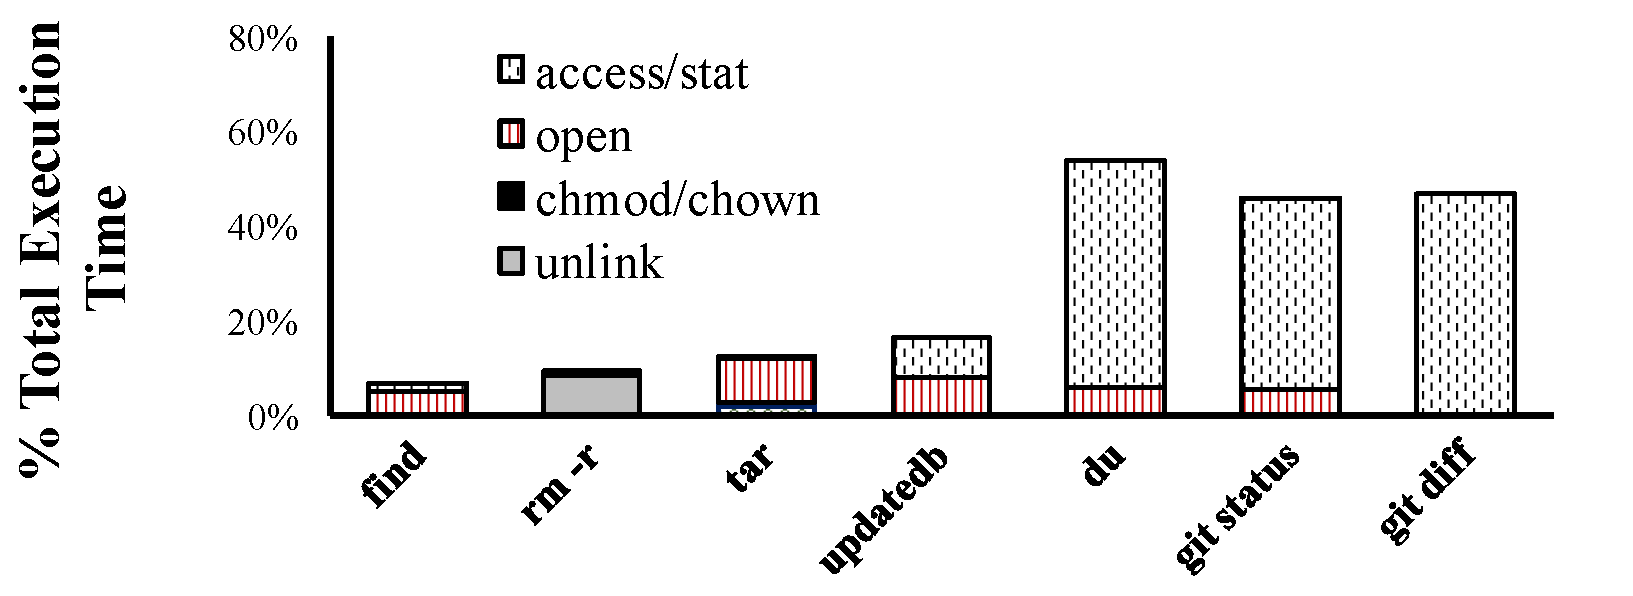
\includegraphics[width=5in]{dcache/plots/syscall-percentage.pdf} \\
\caption[Fraction of execution time on path-based system calls.]
{Fraction of execution time in several common utilities spent
executing path-based system calls with a warm cache, as measured with ftrace.}
\label{fig:dcache:lookup-frac}
%\vspace{-10pt}
\end{figure}

%\fixmedp{Please check these \% against time.  I think git diff is too high.  git status seems ok.}

Directory caches are essential for good application performance.
%Unix was designed such that ``(almost) everything is a file'',
%thus even accesses to in-memory file systems, device files, FIFOs and domain sockets
%first pass through the directory cache.
%In other words, 
Many common system calls must operate on file paths,
which require a directory cache lookup.
For instance, between 10--20\% of all system calls in the iBench system call traces do a path lookup~\citep{filenotafile}. 
Figure~\ref{fig:dcache:lookup-frac} lists the fraction of total execution time
%, as well as system time, 
several common command-line applications spend executing path-based system calls
(more details on these applications and the test machine in \S\ref{sec:dcache:eval}).
We note that these system calls include work other than path lookup,
and that these numbers include some instrumentation overhead;
% are coarse measurements that include  and work than path lookup;
%, and includes some time 
%for synchronous I/O (e.g., during {\tt rename}) as well as non-path tasks (e.g., creating 
%a file handle as part of {\tt open});
nonetheless, in all cases except {\tt rm},
the system call times and counts are dominated by
{\tt stat} and {\tt open}, for which 
%can be serviced from cache and for which 
path lookup is a significant component of execution time.
For these applications, path-based system calls account for 6--54\% of total execution time.
%and 25--77\% of system time.  
This implies that
lowering path lookup latency is
 one of the  biggest 
opportunities for a kernel to improve these applications' execution time.




\begin{figure}[t!]
\centering
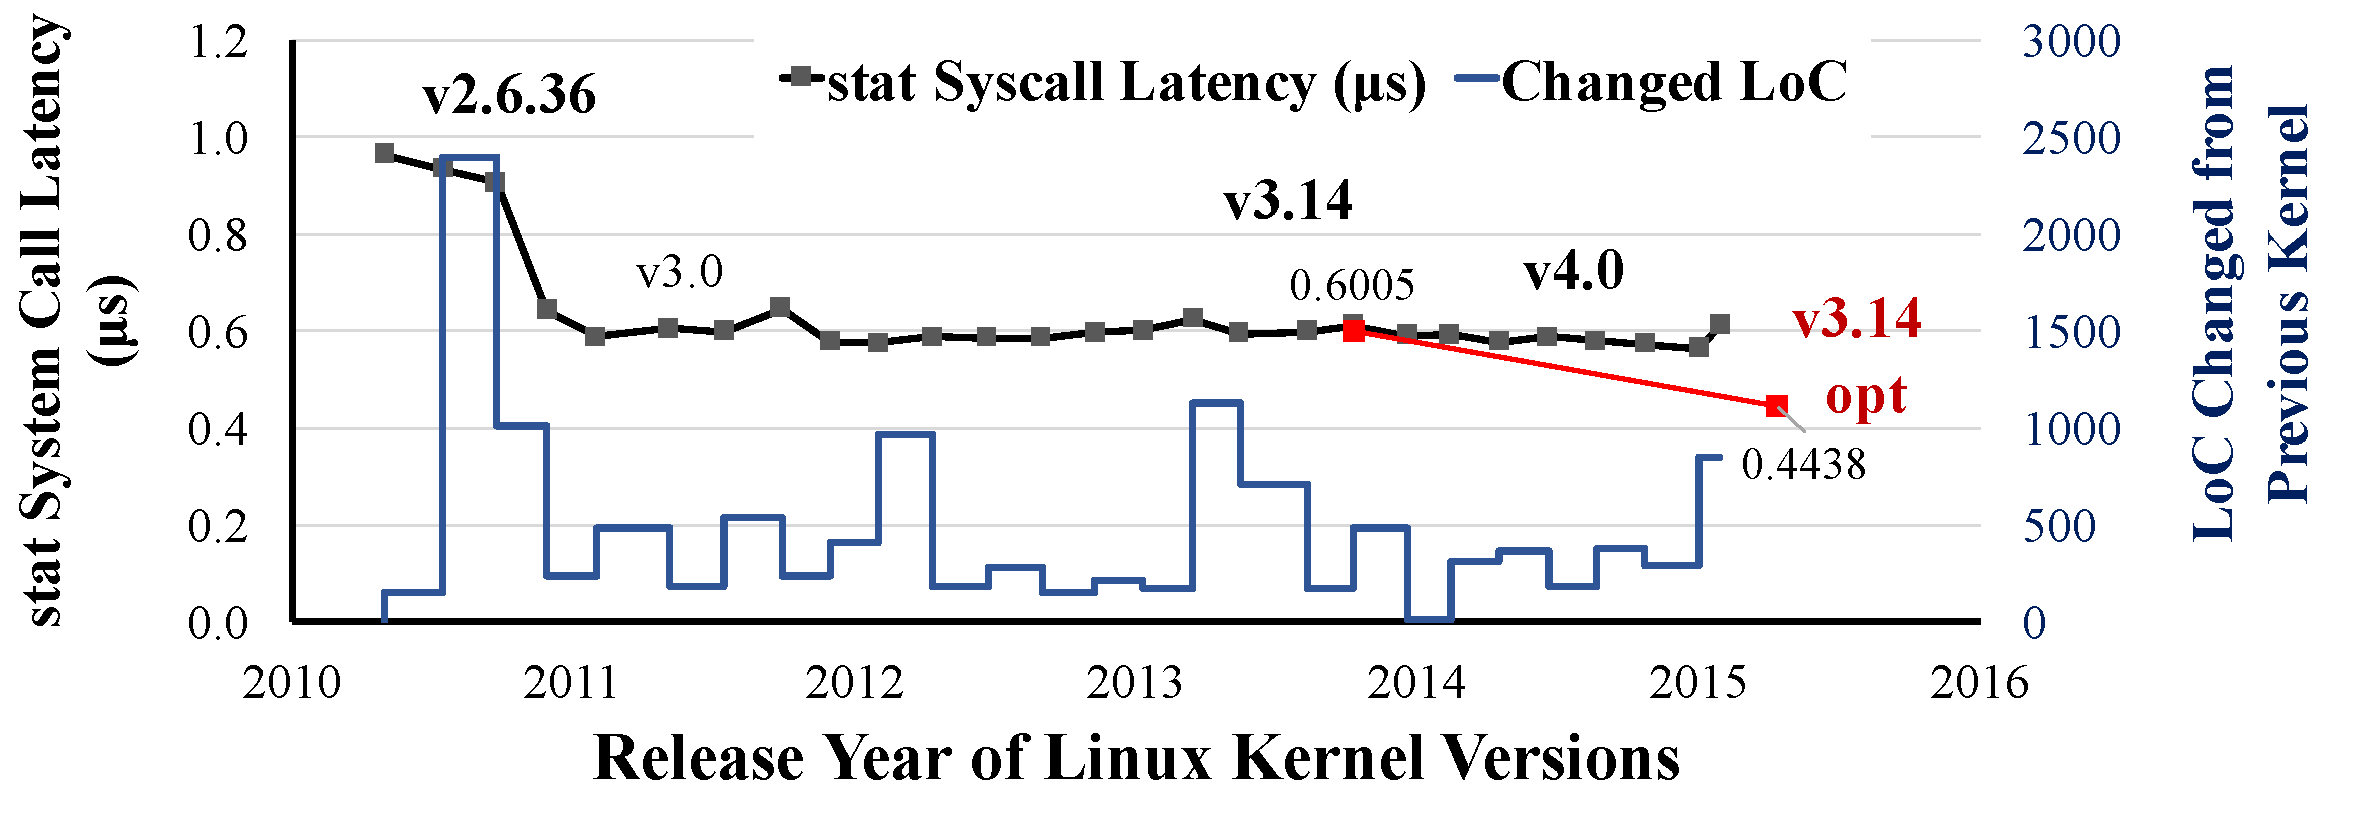
\includegraphics[width=6in]{dcache/plots/latency-by-version.pdf}
\footnotesize
\caption[Lantecy of {\tt stat} system call over years.]
{Latency of {\tt stat} system call with a long path {\tt XXX/YYY/ZZZ/AAA/BBB/CCC/DDD/FFF} on Linux over four years (lower is better), as well as the churn within the directory cache code (all insertions in {\tt dcache.c}, {\tt dcache.h}, {\tt namei.c}, {\tt namei.h} and {\tt namespace.c}). 
%Our optimizations significantly improve performance that has otherwise plateaued, despite significant ongoing developer effort.  
Our optimized \linuxver{} kernel 
further reduces {\tt stat} system call latency by \statspeedup{}\%.}
%\vspace{-15pt}
\label{fig:dcache:by-version}
\end{figure}


%\fixmedp{Add more evidence of lookup importance here: For instance, fraction of lookup time in file-related syscalls, or total lookup time in applications bound on file lookup latency.  }
Unfortunately, even directory cache hits are costly---0.3--1.1 \us{} for a {\tt stat} on our test Linux system, compared to only .04 $\mu$s for a {\tt getppid} and 0.3 \us{} for a 4 KB {\tt pread}. 
%\fixmetsai{Don, check this, I think read will be a better example, getppid is too trivial.}
This issue is taken particularly seriously in the Linux kernel community, which has 
made substantial revisions and increasingly elaborate optimizations to reduce the hit cost
of its directory cache, such as removing locks from the read path or replacing lock ordering with deadlock avoidance in a retry loop~\citep{corbet09jls,dcache-rcu}.
Figure~\ref{fig:dcache:by-version} plots directory cache hit latency against  lines of directory cache code changed 
over several versions of Linux, using a path-to-inode lookup \microbench{} on the test system described
in \S~\ref{sec:dcache:eval}.
These efforts have improved hit latency by 47\% from 2011 to 2013, but have plateaued
for the last three years.
%\fixmedp{if time, filter irrelevant changes from code deltas}
%at the cost of substantial developer effort.
%This latency appears to have plateaued 

The root of the problem is that the POSIX path permission semantics
seemingly require work that is linear in the number of path components,
and severely limit the kernel developer's implementation options.
%The root of this problem is that current directory cache
%designs reflect a straightforward implementation of the POSIX specification,
%which would seemingly require work that is linear in the number of path components.
For instance, in order to open file {\tt /\fnone{}/\fntwo{}/\fnthree{}} 
%for reading, 
one must have search permission
to parent directories {\tt /}, {\tt /\fnone{}}, and {\tt /\fnone{}/\fntwo{}},
as well as permission to access file {\tt \fnthree{}}.
The Linux implementation %of this specification is straightforward, 
simply walks the directory
tree top-down to check permissions.  
Unfortunately, when the critical path is dominated by 
walking a pointer-based data structure, 
including memory barriers on some architectures for multi-core consistency, 
modern CPUs end up stalling on hard-to-prefetch loads.
Moreover, because so many Linux features are built around this behavior, such as Linux Security Modules (LSMs)~\citep{wright+lsm},
namespaces, and mount aliases, it is not clear that any data-structural enhancements
are possible without breaking backward-compatibility with other Linux kernel features.
A priori, it is not obvious that a faster lookup algorithm, such as a single hash table lookup, 
can meet these API specifications and kernel-internal requirements; to our knowledge,
no one has tried previously.

%This paper proposes a decomposition of the directory cache, which allows
%most lookup operations to execute with a single hash table lookup (\S\ref{sec:dcache:dcache}),
%as well as optimizations to reduce the miss rate based on information that is {\em already in the cache}, but not used effectively (\S\ref{sec:dcache:readdir}).
%Our design maintains compatibility (\S\ref{sec:dcache:generalize}) through 
%several essential insights, including 
%how to separate the indexing of paths from checking parent permissions,
%and how to effectively and safely memoize the results of access control checks.


%% This paper proposes several new ways to organize a directory cache, which can yield 
%% substantial performance improvements over the current state of the art.
%% %This paper demonstrates that, despite this developer effort, there is still a substantial 
%% %missed opportunity hiding behind historical, intuitive, but not fundamental design choices.
%% Most of the Linux directory cache design reflects a straightforward implementation of the POSIX 
%% specification. %, with a division of labor that is suitable for mainstream file systems.

%This paper presents an alternative directory cache organization, which 
%improves performance by separating logical tasks, such as separating path indexing from permission checking; yet the design is sufficient to retain compatibility with POSIX.
%In the case of path lookup, 
%this paper demonstrates how 
%a per-component tree walk can be replaced with a single hash table lookup (\S\ref{sec:dcache:dcache}).
% without violating POSIX compliance.

%Our optimizations improve the performance of frequent lookup operations, but 
%introduce several costs, described in \S\ref{sec:dcache:dcache} and measured in \S\ref{sec:dcache:eval},
%which  we believe are acceptable and a net improvement for applications.
%First, these optimizations slow down infrequent modifications to the directory hierarchy, such as {\tt rename}, {\tt chmod},
% and {\tt chown} of a directory. 
%However, these slower operations
%account for less than .01\% of the system calls in the iBench traces~\citep{filenotafile}.
%Second,  the memory overheads of the dcache are increased.
%%(45\% per \dentry{}, as well as some  in our prototype).
%%(\fixmedp{XX MB} in our tests).  
%Third, lookup has a 
%probability of error from signature collisions that can be adjusted to be negligible
%%($2^{-141}$ in our configuration), 
%and within acceptable thresholds widely used by data deduplication systems~\citep{Debnath:2010:CSU:1855840.1855856, Srinivasan:2012:ILI:2208461.2208485, Quinlan:2002:VNA:645371.651321, Zhu:2008:ADB:1364813.1364831}.
%%, as well as how to remove
%%all memory barriers from the lookup path (\S\ref{sec:dcache:update}).
%In the micro-benchmark of Figure~\ref{fig:dcache:by-version}, our directory cache 
%optimizations improve lookup latency by 
%%revisions improve latency of accessing a long path
%%by 
%\statspeedup{}\% over unmodified Linux.
%%Our design addresses other missed
%%opportunities, such as identifying new opportunities to reduce the miss rate
%%through caching directory completeness.
%%\fixmedp{Do we want to highlight LoC?  3K is more than anything in the graph} \fixmetsai{Probably just mention in the evaluation. It's a metric that we should provide, but it's not awfully interesting.}
%%The total lines of code changed are fewer than 3,000 out of \fixmedp{XX}.
%%\fixmedp{Can we get 
%%, yet changes fewer than 3,000 lines of code.

%% SOSP cut - kind of long-winded
\begin{comment}
This paper rethinks current Linux directory cache design choices in light of the following goals:
\begin{compactitem}
\item {\bf Minimize the cost of a cache hit.} (\S\ref{sec:dcache:dcache}).
This means maximizing the benefit of temporal locality for frequent operations,
while pushing extra work of consistency maintenance onto less frequent, already-expensive operations.
%such as handling cache miss or updating massive metadata,
%in order to improve very frequent operations.
\item {\bf Maintain legacy compatibility.} (\S\ref{sec:dcache:generalize}).  Unix path semantics are complex, required by applications, file systems, and security modules, frustrating otherwise straightforward optimizations.  However tempting it may be to redesign path behavior to facilitate caching, path operations must exhibit the same behavior, with lower latency.
\item {\bf Never miss the same request twice in quick succession.} (\S\ref{sec:dcache:readdir}).  A number of less-frequent operations, such as reading a directory or secure temporary file creation, always miss in the cache {\em even if enough information is in cache to satisfy the operation.}  
%Of course, infrequent accesses should still be subject to a cache replacement policy, such as LRU.
\end{compactitem}
%Although directory caches must implement more complex semantics than a hardware memory cache,
%these principles should seem familiar to the reader with a basic architecture background.
%sadly, the Linux directory cache design violates all three.
\end{comment}

%This paper introduces several techniques to improve the performance of a directory cache,
%This paper explains several practical directory cache optimizations,
This paper demonstrates that these techniques improve performance for applications that use the directory cache heavily,
and the harm is minimal to applications that do not benefit.
%and that the worst case \microbench{} is only 12\% slower within \fixmedp{XX}\% of unmodified Linux.
%Each optimization we describe improves performance in isolation, and all can be combined.
%These optimizations change very few lines of code, and are backward-compatible with 
%legacy applications.  
%These changes are encapsulated in the VFS---individual file systems do not have to change their code.
%This paper describes a  prototype of these improvements implemented in Linux \linuxver{}.
%\S~\ref{sec:dcache:background} explains that the directory cache structure of Mac OS X, FreeBSD, and Solaris 
%are sufficiently similar that these principles should generalize.
%we compare and contrast Linux's directory cache
%with Mac OS X, FreeBSD, and Solaris in \S\ref{sec:dcache:background}, and explain inline how each
%optimization could be generalized to these other OS kernels.





%% \item {\bf Modularization and stackability}:
%% Any changes or optimizations must be implemented as modules inside Linux's VFS,
%% and can be stacked on top of the original design or any future optimizations. 
%% \item {\bf Backward compatibility}:
%% Any changes or optimizations must maintain least requirement of modifying any
%% file systems.
%% \item {\bf Generalization to other OSes}: Any changes or optimizations must be portable to other OSes with reasonable effort and change of design.




%% \dcache{} is proven to be effective on improving storage performance.
%% Experiments shows that,
%% in a Linux 3.x kernel, a \dcache{} with a xxx\% hit rate can speed up
%% metadata lookup and fetching time by xxx times.
%% \fixmetsai{experiment result, Linux version, and fs specs here}
%% However, we observed that Linux maintainers have made
%% constant and non-trivial efforts to improve \dcache{} in the Linux kernel.
%% We studied all \dcache{}-related source files in the Linux kernel Git repository,
%% and discovered that maintainers have committed
%% on average xxx revisions per source files.

%% We tested metadata lookup time on primary \dcache{}-related revisions.
%% Most changes on \dcache{} system only create xxx\%-xxx\% speed-up
%% than their predecessor.
%% \fixmetsai{result and graph here}.
%% Moreover, improvement to \dcache{} is still work-in-progress
%% for Linux maintainers.
%% \fixmetsai{reference to threads for latest dcache discussions}. 
%% All the evidences show that,
%% despite of significant reduction of storage operations,
%% efficiency of \dcache{} system internally still remains as a concern.

%% We argue that the design of \dcache{} needs to be carefully re-examined,
%% to fundamentally identify any missed opportunities that
%% improve value of \dcache{}.
%% At a high level, most optimization works for \dcache{} are focused on
%% improving ``how to cache'',
%% but we want to also lay eyes on ``what to cache'',
%% to ensure any valuable information returned from file systems
%% be captured by \dcache{} system.

%The contributions of this paper are as follows:
%\begin{compactitem}
%\item A performance analysis of the costs of path lookup and the opportunities
%to improve cache hit latency.
%\item A directory cache design that improves path lookup latency with a combination of techniques, including:
%  \begin{compactitem}
%  \item Indexing the directory cache by full path, reducing average-case lookup from linear to constant in the number of path components.
%  \item A Prefix Check Cache (PCC) that separates permission checking from path caching.  The PCC memoizes permission checks, and is compatible with LSMs~\citep{wright+lsm}.
%  \item Reducing the cost of checking for hash bucket collisions with path signatures.
%  \end{compactitem}
%\item Identifying opportunities to leverage metadata the kernel already has to reduce miss rates, such as tracking whether a directory is completely in cache.
%\item Carefully addressing numerous, subtle edge cases that would frustrate rote application of these techniques, such as integration with symbolic links and Linux namespaces.
%\item A thorough evaluation of these optimizations.  For instance, our optimizations improve throughput
%of the Dovecot IMAP server by up to \dovecotspeedup\% and latency of 
%updatedb by up to \updatedbspeedup{}\%.
%%git version control system by up to 25\%.
%
%\end{compactitem}

\section{Background}
\label{sec:background}

This section summarizes \sgx{},
and current design points for running or porting applications on \sgx{}.
%and the legacy frameworks of porting 
%including \haven{}~\cite{baumann14haven}, \scone{}~\cite{osdi16scone}, and Panoply~\cite{shinde17panoply}. 


\subsection{Software Guard Extensions (SGX)}
\label{sec:background:sgx}

%\begin{figure}[t!]
%\centering
%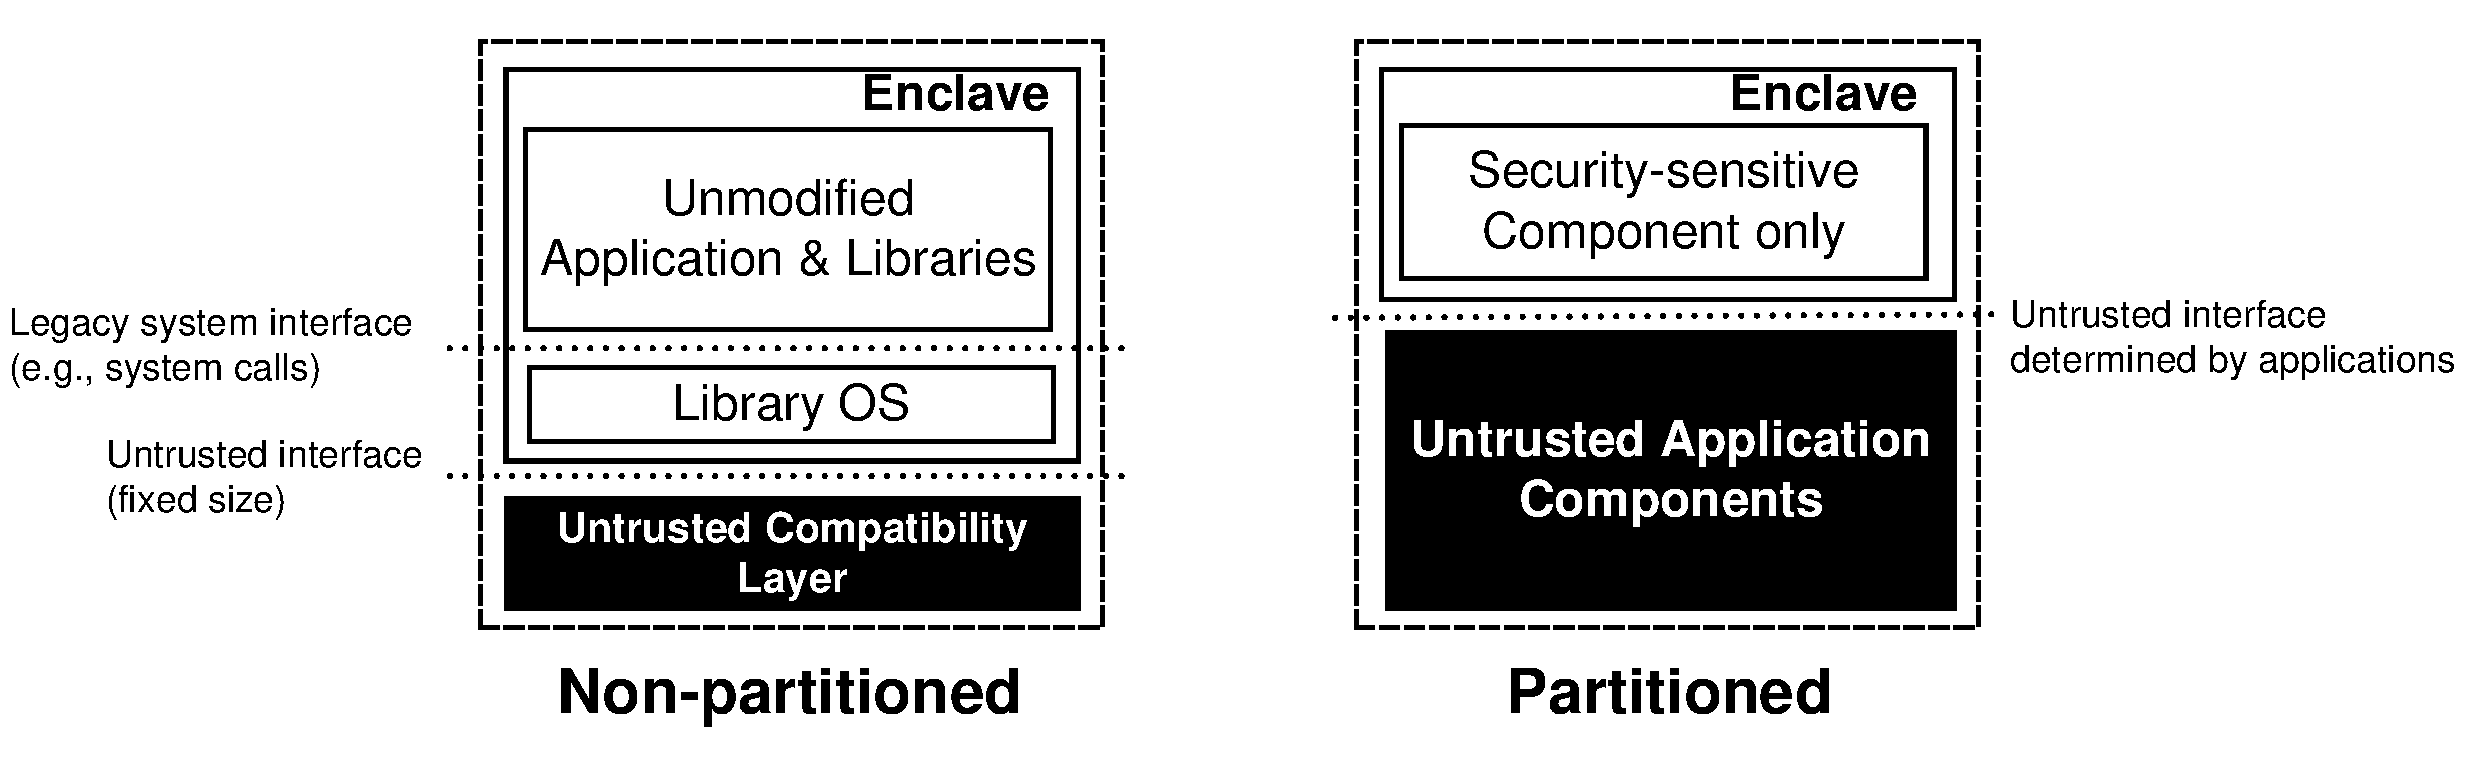
\includegraphics[width=\linewidth]{figures/libosvssdk.pdf}
%\footnotesize
%\vspace{-0.3in}
%\caption{
%Comparison between libOS-based model (e.g., \haven{} and \graphenesgx{})
%and SDK-based (SDK for \sgx{}) model for migrating applications in enclaves.
%Green (light) boxes are trusted components and red (dark) boxes are untrusted.
%The libOS-based model often yields a larger TCB in the enclave,
%while the SDK-based model requires developers to be responsible of
%securing the enclave on the untrusted interface.
%}
%\label{fig:libosvssdk}
%\end{figure}

The primary SGX abstraction is an \emph{enclave}: an isolated execution environment within the virtual address space of a process.
The code and data in enclave memory do not leave the CPU
package unencrypted; when memory contents are read back into cache,
the CPU decrypts the contents, and checks the integrity of cache lines and the virtual-to-physical mapping.
SGX also cryptographically measures the integrity of enclaves at start-up, and 
provide attestation to remote systems or other enclaves.
%Remote entities can identify the owners of enclaves by distinguishing the cryptographic measurements
%generated with different signing keys.

%%% \sgx{} is a new feature on the 6th-genaration \intel{} CPUs.
%%% it contains a set of new x86/64 instructions, to initiate, destroy, and attest isolated execution environments (i.e., enclaves) in the address space of applications.
%%% When \sgx{} loads an application in an enclave,
%%% the code and data of the application will remain encrypted in the main memory,
%%% forbidding any mean to eavesdrop the application secrets.
%is a set of new x86/x64 instructions introduced
%to the latest \intel{} CPUs,
%to bootstrap an isolated execution environment
%inside applications' virtual memory address space.
%\sgx{} creates a memory region
%(generally referred as {\bf enclave}), storing both the code and data of the isolated execution,
%which stays encrypted in DRAMs and only the CPU is capable of encryption and decryption.
%The CPU derives the encryption key
%from the cryptographic measurement of the initial state of enclave memory,
%to allow remote entities to verify the soundness of execution and establish the trust
%needed for provisioning sensitive data.

\sgx{} enables a threat model where one only trusts the \intel{} CPUs and the 
code running in the enclave(s).
%whereas the rest of application, system software, off-CPU-package hardware devices and providers are untrusted. 
\sgx{} protects applications from three different types of attacks on the same host, which are summarized in Figure~\ref{fig:sgx-threats}: untrusted application code inside the same process but outside the enclave; operating systems, hypervisors, and other system software;
%\fixme{added Mona's suggestion}
other applications on the same host; and off-chip hardware.
A SGX enclave can also trust a remote service or enclave, and be trusted after inter-platform attestation~\cite{sgx-attestation}.




%%% \begin{compactenum}

%%% \item {\bf Inside process memory:}
%%% \sgx{} partitions the application process into two privilege levels, as the trusted part (in enclaves) which can access the whole process memory, and the untrusted part (outside enclaves) forbidden to access enclave memory.
%%% %the privileged part (in the  enclave region) can access all process memory,
%%% %while the unprivileged part (outside the enclave region) is limited to access only data that are not isolated by \sgx{}.

%%% \item {\bf From hosting OSes or hypervisors:}
%%% \sgx{} assumes that OSes and hypervisors can be compromised by either exploiting system vulnerabilities
%%% or malicious system software installed by administrators.
%%% Both types of compromise are legitimate threats to modern OSes, due to complexity of modern OSes and usage of public facilities like clouds.

%%% %Operating systems or hypervisors
%%% %that are either compromised by rootkits
%%% %or deliberately modified by the host providers.
%%% %An attacking host can access the raw data in DRAMs, or remap the
%%% %physical pages to other contexts.

%%% \item {\bf Physically from the hardware:}
%%% One type of attacks that cannot be defended by software-based solutions~\cite{flicker, criswell2014virtualghost}
%%% is from the attackers who have physical access to the hosts.
%%% \sgx{} can resist attacks on the host hardware
%%% including hacking peripheral devices like ethernet cards and connectors~\cite{hudson15thunderstrike}, tapping into buses, or eavesdroping DRAM data using Cold-boot attack~\cite{halderman09coldboot}.


%%% \end{compactenum}


%%% \sgx{} protects an application against unpredictable threats from both local and remote hosts.
%%% \sgx{} establishes a trusted path
%%% from one enclave to another,
%%% providing end-to-end protection to both enclaves to
%%% exchange data with confidentiality and integrity.
%%% %, processing the data and returning the computation results with end-to-end protection.
%%% We can further divide up the protection using \sgx{} into three elements:
%The use cases of \sgx{} mostly involve the process that an enclave
%retrieves a signed attestation from the processor,
%to exchange provisioning of critical information from remote servers.
%The purpose of such process is equivalent to
%expanding the trusted execution
%from remote servers
%to untrusted hosts,
%to harness resources such as CPU cycles and DRAMs.

%%% \begin{compactenum}

%%% \item {\bf Isolated execution:}
%%% \sgx{} guarantees the execution initiated in an enclave
%%% to be isolated from any part of the system except the enclave itself.
%%% %any part of the system except the enclave itself can access the execution state. 
%%% Achieved by the secrecy of encryption keys in \intel{} CPUs.

%%% \item {\bf Attestation of integrity:}
%%% Remote entities with a \sgx{}-enabled CPU can verify the integrity of an enclave, using the \intel{} Attestation Services (ISV)~\cite{isv}.
%%% %for its integrity of running the exact code that it is given.
%%% Achieved by the uniqueness of CPU keys to sign the cryptographic measurement of enclaves.

%%% \item {\bf Authentication:}
%%% Remote entities can identify the owners of enclaves by distinguishing the cryptographic measurements generated with different signing keys.


%%% %explicitly launched for processing the specific tasks, regardless of the identicality of execution.
%%% %That is, two mutually distrusting users can launch the same execution in  separate enclaves, yet be able to distinguish by the measurements as MACs (Message Authentication Code) signed by the users' private keys.

%%% \end{compactenum}


%One must note that \sgx{} only promises the integrity of application binaries
%initially loaded in enclaves.
%The gap between integrity of binaries and complete security has to be filled
%by ones who develop and approve the applications.
%More specifically, the clients are responsible of
%testing whether the applications contain any vulnerabilities
%that lead to information leak.
%To minimize the risk of leaving any flaws in the applications unintentionally,
%developers often tend to cut down the trusted computing base (TCB)
%of the applications. With smaller TCB, clients who launched the enclaves
%can more easily reason about the thoroughness of securing the execution.

%To achieve smaller TCB, the software development kit of \sgx{}
%intends to encourage developers to partition the applications and
%keep only security sensitive components in the enclaves.
%Such an intention is exactly contradicted by the trust model of \haven{},
%which must trust the loaded application as a whole.
%Except for the cases in which the whole applications must be secured,
%\haven{} actually downgrades the trustworthiness of enclaves.
%Figure~\ref{fig:libosvssdk} shows the comparison of the two models.


%%% By synthesizing and streamlining these three elements (i.e., isolation, attestation and authentication),
%%% \sgx{} provides a promising build block to securing applications
%%% from unpreditable security threats.

%developing applications
%that are resistant to unpreditable, unavoidable threats.
%Users expect \sgx{} to build up a wall for protecting the sensitive data, even against a catastrophic scenario like a complete takeover of the infrastructure.  

%\fixmedp{Explain how to read the figures in the captions. What do colors and shading mean?}
%
%\fixme{Disabled the whole discussion about SDK. dp: ok with me, but probably drop from figure} 
\begin{comment}
\subsection{The legacy framework (The \sdk{})}

{\bf Intel's \sgx{} SDK} (software development kit) for Linux~\cite{intel-sgx-sdk} is the official framework
for programming \sgx{} execution within Linux applications.
\sdk{} includes the components of two phases:
a {\bf compile-time utility} to generate a valid executable for running inside enclave,
and a {\bf run-time framework} to trigger the hardware-enforced isolated execution.
The two-phased design is based on the assumption that compilation of applications
is controlled by trusted, security experts,
to retain the trustworthiness of isolation model when running on untrusted OSes.


The work flow of \sgx{} programming using \sdk{} is as follows:
\begin{compactenum}
\item At the build-time (on trusted hosts), developers create a self-contained, static executable as the initial code and data after enclave creation.
We refer the executable as an ``enclave image''.
The enclave image is statically links with the enclave infrastructure, which provides enclave APIs (e.g., retrieving attestation) and a extremely small set of POSIX functions (e.g., {\tt memset()}).
After linking, the compile-time utility signs the executable and inserts the enclave signature structure
({\tt SIGSTRUCT}) in the application code.
\item At the execution-time (on untrusted hosts), the enclave image is taken by the framework. The user-space driver then requests enclave creation with the kernel driver, through {\tt ioctl()} to a pseudo-device {\tt /dev/isgx}.
The kernel driver creates and initializes an enclave using the authenticated signature structure,
and a token exchanged from an architectural enclave, {\tt AESMD}, for ensuring the validity of enclave. 
\end{compactenum}





%During the compile time,
%the developers create a self-contained, static binary, as the initial image of an run-time enclave (an ``enclave image'').
%\sdk{} provides the infrastructural libraries (libsgx) for static linking, which contain enclave APIs and few POSIX functions.
%A signing tool of \sdk{} will generates a valid enclave signature
%derived from the enclave image.
%Both the static linking and signing must happen on a trusted, development machine.


%After generating the enclave image, developers then ship it with the rest of application,
%to untrusted hosts (\sgx{}-enabled)
%where the \sdk{} run-time framework is installed.
%The run-time framework provides both kernel and user-space drivers,
%to interface \sgx{} hardware using the new x86 instructions (e.g., {\tt ECREATE}, {\tt EADD}, {\tt EENTER}).
%The framework also includes an architectural enclave (AESM), for validating the enclave attributes (and generating a run-time token),
%and a kernel EPC (enclave page cache) driver that manages paging for all running enclaves.



% includes both compile-time and run-time components:
%for the compile time, the SDK provides all the infrastructure libraries,
%which the applications statically link with,
%and a signing tool that generates the enclave signatures for hardware validation.
%The run-time framework then takes the signed enclave binaries,
%and uses the kernel and user-space drivers to initiate the isolated execution in enclaves.



\sdk{} centers the whole programming model based on the concept of partitioning an application,
and isolating only minimum application code in enclaves.
The partitioning minimizes the risk of compromising the enclaves,
due to smaller trusted computing base (TCB) and less opportunity of omitting security glitches.
With this model,
developers are expected
to identify the part of an application that performs the sensitive operations,
and define an validated interface to
the sensitive part and rest of the application.
\sdk{} encourages partitioning by reducing the difficulty of defining and accessing the interface---a language tool automatically generates the interface code with extra argument-sanitizing code.
The generated interface code essentially filters input and output of the enclave,
and prevents randomly copying memory across the enclave boundary, leaking or corrupting internal data.


%The Intel SDK has its limitations. The infrastructure of the SDK provides APIs in enclaves for accessing SGX features (e.g., attestation), as well as a small set of POSIX APIs
%(\roughly{}10 functions, such as {\tt printf} and {\tt memset}).


Despite that \sdk{} attempts to alleviate the difficulty of partitioning for SGX,
porting a piece of application code that is sophisticated and interactive to the rest of application
is still a significant cost to pay.
In general, developers want to find a reasonable granularity of partitioning---a ``sweet spot'' that partitions the application code neither too small nor too large, 
to nicely balance between frequency of enclave exits and risk of introducing incompatible code.
For an application written in C/C++, partitioning is cumbersome especially if the application is poorly modularized.


Unfortunately, the limited POSIX support in the \sdk{} infrastructure really strikes
the opportunity of fine-grained partitioning.
The lack of POSIX APIs in the infrastructure is fundamental, due to the restriction
on OS interaction from the enclaves.
The missing APIs encapsulates system calls, which can expose the enclave to some risky OS interaction model, such as {\bf Iago Attacks}~\cite{checkoway13iago}.

%In conclusion, this work targets on completing the API support, either at POSIX level or system calls,
%while retaining the isolation model.
%The platform can assist developers to refocus on partitioning applications for minimizing the risks.

\end{comment}

\subsection{SGX Software Design Space}

This subsection summarizes the principal design choices facing any 
framework for running applications on SGX.  We explain the decisions in
recent systems for SGX applications, and the trade-offs in this space.

\begin{figure}[t!]
\centering
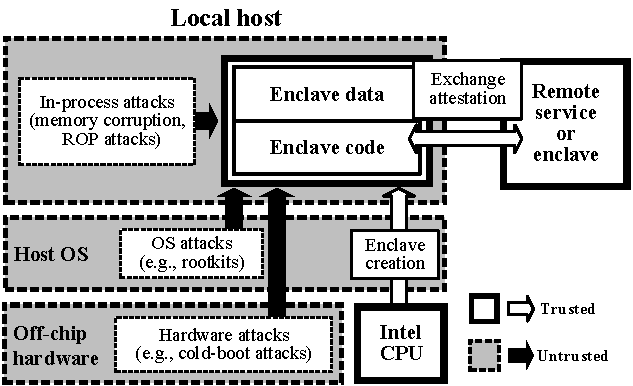
\includegraphics[width=.5\linewidth]{sgx.pdf}
\caption{The threat model of \sgx{}. \sgx{} protects applications
from three types of attacks:
in-process attacks from outside of the enclave,
attacks from OS or hypervisor, and attacks from off-chip hardware.}
% Red (dark) boxes are untrusted components and green (light) boxes are trusted.}
%For each enclave, \sgx{} establishes the chain of trust from the \intel{} CPU.
%Enclaves across physical machines or even infrastructures can remotely attest the integrity of execution, using the signatures generated and signed by the CPU.
%Green (light) boxes and arrows represent the trusted components and operations, and red (dark) boxes and arrows represent the otherwise.
\label{fig:sgx-threats}
\end{figure}

\paragraph{How much functionality to pull into the enclave?}
At one extreme, a library OS like Haven~\cite{baumann14haven} pulls most
of the application-supporting code of the OS into the enclave.
On the other extreme, thin ``shim'' layers, like SCONE~\cite{osdi16scone} and Panoply~\cite{shinde17panoply} 
wrap an API layer such as the system call table.
Pulling more code into the enclave increases the size of the TCB,
but can reduce the size and complexity of the interface, and attack surface, 
between the enclave
and the untrusted OS.

The impact of this choice on performance
largely depends on two issues. First, entering or exiting the enclave 
is expensive; if the division of labor reduces enclave border crossings, 
it will improve performance.
The second is the size of the Enclave Page Cache (EPC),
limited to 128MB on version 1 of SGX.
If a large supporting framework tips the application's working set size
past this mark, the enclave will incur expensive swapping.


\paragraph{Shielding complexity.}
SGX hardware can isolate an application from an untrusted OS, but 
SGX alone can't protect an application that  requires
functionality from the OS.  {\em Iago attacks}~\cite{checkoway13iago}
are semantic attacks from the untrusted OS against the application, where an unchecked system call return 
value or effect compromises the application.
Iago attacks can be subtle and hard to comprehensively detect, at least with the current
POSIX or Linux system call table interfaces.

Thus, any SGX framework must provide some {\em shielding} support, to 
validate or reject inputs from the untrusted OS.  
The complexity of shielding is directly related to the interface complexity:
inasmuch as a library OS or shim can reduce the size or complexity of the 
enclave API, 
the risks of a successful Iago attack are reduced.

\paragraph{Application code complexity.}
Common example applications for SGX in the literature 
amount to a simple network service running a TLS
library in the enclave, putting minimal demands on a shim layer. 
Even modestly complex applications, such as the R runtime and a simple
analytics package, require dozens of system calls providing wide-ranging functionality, 
including \syscall{fork} and \syscall{execve}.
For these applications, the options for the user or developer become: 
(1) modifying the application to require less of the runtime; (2) opening and shielding more 
interfaces to the untrusted OS; (3) pulling more functionality into a shim or a library OS.
The goal of this paper is to provide an efficient baseline, based on (3),
so that users can quickly run applications on SGX, and developers can 
explore (1) or (2) at their leisure.

\paragraph{Application partitioning.} An application can have multiple
enclaves, or put less important functionality outside of the enclave.
For instance, a web server can keep cryptographic keys in an enclave,
but still allow client requests to be serviced outside of the enclave.
Similarly, a privilege-separated or multi-principal application might create a separate enclave for
each privilege level.

This level of analysis is application-specific, and beyond the focus of this paper.
%which is on running unmodified applications in enclaves.
However, partitioning a complex application into multiple enclaves
can be good for security. In support of this goal,
\graphenesgx{} can run smaller pieces of code, such as a library, in an enclave, as well as
coordinate shared state across enclaves.

%* Partitioned vs. unpartitioned app?

%** Right choice depends a lot on whether the app has multiple principals or security concerns.

\begin{comment}
\fixmedp{Did a first cut at 2.2; needs to integrate the figure (or drop it).  I didn't know what to write for 2.3 yet.  I left the old text below for now (if there is anything you really want to save), but it needs to go away}

\subsection{Open Challenges}

\fixmedp{Here, I would give a taste of some of the issues we solve and why they are hard, like dynamic loading (and maybe fork or IPC).  Keep it short, a few paragraphs.}
\end{comment}

%\begin{figure}[t!]
%\centering
%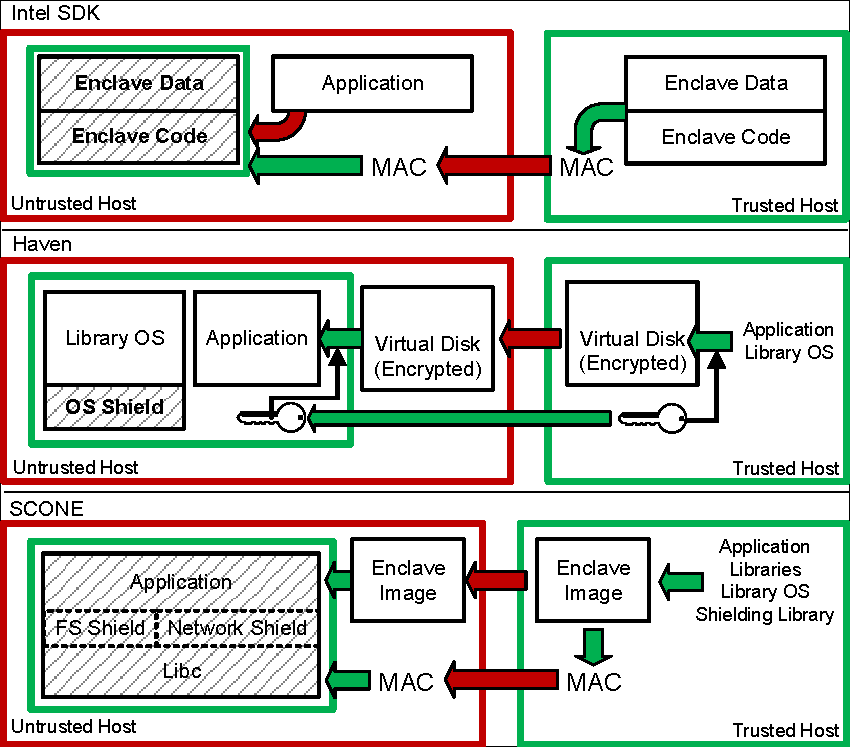
\includegraphics[width=\linewidth]{figures/sdkvslibos.pdf}
%\caption{Comparison of the code integrity model among different \sgx{} frameworks, including the \sdk{}, \haven{} and \scone{}.}
%%Green (light) boxes and arrows represent the trusted components
%%and operations, and red (dark) boxes and arrows represent the otherwise.
%%Patterned blocks represent the code and data included in the initial measurements of the enclaves.}
%\label{fig:sdkvslibos}
%\end{figure}


\begin{comment}
\subsection{\sgx{} shielding systems}
\label{sec:background:shielding-systems}




The current \sgx{} shielding systems, such as \haven{}~\cite{baumann14haven}, \scone{}~\cite{osdi16scone}, and Panoply~\cite{shinde17panoply}, enforce end-to-end isolation to
legacy applications without partitioning.
A \sgx{} shielding system preserves the trusted computing base (TCB)
of an application, and further increases it with a shielding layer to defend against the untrusted OSes.
By avoiding application partitioning,
%model of quarantining an unmodified, COTS application in an \sgx{} enclave.
a shielding system minimizes the effort of reprogramming the applications for \sgx{} execution, often with recompilation or packaging the binaries in an encrypted enclave.
%to merely recompiling or packaging the application code before signing it off for enclave execution.
%These \libos{}es internalize OS features into the enclave, to maintain a fixed-size,
%narrow interface to the untrusted host OSes.
%Porting applications using a \sgx{} \libos{} is vastly different from the programming model of \sdk{}---no programming effort is needed when porting with a \sgx{} \libos{}, and applications are isolated without partitioning.
In the following paragraphs, we compare the current shielding systems with the \graphenesgx{} approach.

\haven{}~\cite{baumann14haven} uses a \libos{} called \drawbridge{} in each enclave
to shield a single-process \emph{Windows} application from the untrusted host OS.
\haven{} absorbs the implementation of system APIs (i.e., Win32 APIs) from the host OS,
%\haven{} uses \drawbridge{}~\cite{porter11drawbridge} as the backbone of its enclave infrastructure, 
and exports a narrow enclave interface on which untrusted inputs are carefully filtered to defend against the Iago-type attacks.
Adding a \libos{} to each enclave causes a bloat of TCB---for \haven{}, the size of a \libos{} binary and shielding layer is \roughly{}200MB.
\haven{} has to establish the trust and integrity in all these binaries loaded into an enclave. Except that the shielding layer is a part of the enclave since its creation, \haven{} enforces the integrity of both the \libos{} and the isolated application,
by storing all binaries on an encrypted virtual disk and relying a remote, trusted server to provision the key for decryption.
\haven{} builds a trusted path from a remote server to local cloud machines,
to securely bootstrap application execution inside the enclaves.
%Other minor comparison between \haven{} and this work: the development and evaluation of \haven{}, at publication, is based on a simulated architecture.
%On the contrast, \graphenesgx{} is a released open-source platform, tested by many developers from institutes and corporations. \fixme{maybe bring up TCB?}



\scone{}~\cite{osdi16scone} isolates Linux micro-services in enclaves as a container-like environment.
After a brief attempt of building a \libos{} like \haven{},
\scone{} chooses a different approach of shielding the system API usage in applications, by designing shielding strategies based on each API.
\scone{} stacks the application on top of file-system and network shielding libraries, and extends a standard library C (musl~\cite{musl}) to securely exit the enclave for system calls.
Within the \sgx{}-aware Libc, \scone{} carefully filters the inputs from the host system calls, as the defend against known Iago attacks.
For instance, \scone{} ensures that pointers given to and returned by a host system call will point to addresses outside the enclave,
to prevent the host OS to manipulate pointers and cause memory corruption in the enclave.
\scone{} also authenticates or encrypts file or network streams
based on configurations given by the developers.


%The \libos{} implementation in \scone{} is based on musl~\cite{musl} and LKL (Linux kernel library)~\cite{lkl}.
%The design of a SCONE enclave (or Secure Container) has similarity
%with a basic block of \graphenesgx{}:
%they both validate input files based on cryptographic methods, and are fully configurable at a per-file basis.
%However, \graphenesgx{} supports a more complete set of Linux system APIs.
%The APIs that \graphenesgx{} especially contributes over \scone{} are the Linux multi-process APIs, including copy-on-write {\tt fork()}, {\tt exec()}, signals, and system V IPC (message queues and semaphores).

Panoply~\cite{shinde17panoply} further reduces the TCB of a shielding system over the SCONE approach, by excluding both a \libos{} and \libc{} from enclaves.
Instead, Panoply uses a shim layer shielding a portion of the POSIX API. The shim layer yields about 20 KLoC as its TCB (trusted computing base), which is much smaller than libc and/or a library OS.
% in other shielding systems.
As Panoply delegates the libc functions outside the enclave, its shim library defends the supported POSIX API,
including 91 {\em safe} functions and 163 {\em wild (unsafe)} functions.
Panoply also supports multi-process API including \fork{}, \exec{}, signaling, and sharing untrusted memory with inline encryption.
Compared to \graphenesgx{}, Panoply has made some different design decisions in supporting multi-process API,
including supporting fork by copying memory on-demand with statically determining memory access,
and using secured messaging for inter-process negotiating instead of coordinating over an encrypted RPC stream.




\subsection{Comparison and security implications}

\fixme{need to drop the SDK discussion, revisit the security claims, and discuss Iago attacks in details.}

Figure~\ref{fig:sdkvslibos} shows the comparison between \haven{}, \scone{}, Panoply, and \graphenesgx{}.
%The \sdk{} model uses a static MAC of the enclave code and data, given to the \sgx{} driver for bootstrapping the isolated execution.
The \haven{} model only initiates enclaves with the OS shield layer,
which unpacks the enclave binaries from a virtual disk---decrypted using a provisioned key.  
The \scone{} model extends the \sdk{} model---it statically links the application binaries with the shielding library, creating a static enclave image verifiable by its MAC. The \sdk{} and \scone{} model retain more flexibility in deploying and integrating \sgx{} enclaves by focusing on the code integrity rather than encryption.

The key concerns that affects users choosing among these solutions are {\bf trusted computing base (TCB) size} and {\bf attack surface}.
However, since all these solutions are based on different design decisions, assumption and requirements, the comparison of TCB size and attack surface is often imprecise and inconclusive.

\paragraph{TCB size.}
Most studies measure the TCB size of a system by the total LoC (lines of code) written for all the trusted components, or the size (in bytes) of all the trusted binaries.
The comparison of TCB size is only meaningful when two systems have comparable system features,
and are order-of-magnitude different in term of LoC or binary size.
For instance, the comparison of TCB size between \haven{} and \scone{} is never an apples-to-apples comparison.
The implemented system features and personalities
in these two systems are fundamentally different, and \haven{} supports a much larger fraction of Windows features than the fraction of Linux features supported by \scone{}.

We argue that the only occasion that the reduction of TCB size
can be convincingly demonstrated is when a design has partitioned a system into isolated components,
or removed unreachable execution paths.
For instance, the \sdk{} promotes application partitioning for \sgx{};
it requires additional partitioning effort but is effective for confining the TCB size.
By statically linking the application binaries
with the shielding layers and standard C library, \scone{} offers more opportunities in stripping the Libc and shield code of unused APIs, and thus reducing its TCB size.



\paragraph{Attack surface.}

Most studies estimate the severity of having an attack surface by the size of interface to the trusted and untrusted components.
The experience of \scone{} provides an important insight for estimating attack surface: the narrowness of interface is not proportional to the difficulty of defending against incoming attacks.
An interface overloaded with too many features or semantics can become a major source of vulnerabilities.

%\subsection{The \graphene{} Library OS}
%
%\graphene{}~\cite{tsai14graphene} introduces a \libos{} design that supports
%both single-process and multi-process Linux applications,
%but retains a narrow host interface (43 functions) as a vantage point for enforcing security isolation.
%The main contribution of \graphene{} is an distributed implementation of the POSIX namespace coordination,
%to support Linux multi-process abstractions across \libos{} instances.
%All the multi-process abstractions in \graphene{} is implemented using simple pipe-like RPC streams,
%without relying on any host memory sharing support.
%Based on this design, \graphene{} can easily isolate mutually untrusting applications,
%by blocking the RPC streams between unrelated applications.
%
%
%
%The design decisions made by \graphene{} are important keys to the \graphenesgx{} framework.
%First, the host interface contains mostly internal abstractions, and three external ones including files, network connections, and RPC streams.
%The simplicity of the host interface facilitates shielding the \libos{}
%from risky OS interaction.
%Moreover, \graphene{} implements multi-process abstractions across instances without memory sharing.
%\graphenesgx{} can rely on the distributed POSIX implementation
%to support multi-process applications across multiple enclaves, by coordination over validated RPC streams.


\end{comment}




\papersection{Security isolation}
\label{sec:linux:security}

\issuedone{1.1.d}{Describe the security isolation story for Linux hosts}
\graphene{} separates OS features from security isolation.
This section explains the Linux host design for isolating mutually untrusting applications, with a reduced attack surface for protecting Linux kernels.
The discussion starts with the security guarantees and threat model, followed by the technical details of security isolation on a Linux host.



\papersubsection{Goals and threat model}

The security isolation model of \graphene{} ensures that mutually-untrusting applications cannot interfere with each other.
A goal of \graphene{} is to provide security isolation with comparable strength as
running applications in separate VMs.
When running two unrelated applications on the same machine,
the security requirement
of the OS involves not only blocking unauthorized access under normal circumstance,
but also preventing an application
from maliciously exploiting OS vulnerabilities to attack the other application.
Because a modern OS, such as Linux or \win{}, contains a rich of features and APIs,
it is difficult to eliminate OS vulnerabilities
or even just to verify whether an OS contains any vulnerabilities. 
A Linux container~\cite{lxc}
does provide a separate OS view for each application,
but still relies on the correctness of the whole Linux kernel to enforce security isolation.
On the other hand, a VM or a \libos{}
isolates the whole OS kernel or a part of the kernel in an unprivileged guest space
for each application.
The security isolation model prevents
any vulnerabilities inside the VM or the \libos{} from compromising the host kernel and other applications.



\graphene{} enforces security isolation %between applications
by separating 
backward-compatible OS features from security mechanisms.
A Linux kernel exports a wide range of system calls,
either as a legacy of previous kernels or as new programmability features. % of newer kernels.
By implementing OS features in a \libos{},
\graphene{} reduces the attack surface of a Linux kernel
to a small amount of system call corner cases.
%to implement \thehostabi{}.
%If a machine only runs applications in \graphene{},
%a Linux developer can try to carve out a minimal Linux kernel, containing only features needed by the Linux PAL.
A reduced attack surface
eliminates majority of execution paths inside a Linux kernel in which a malicious application can explore for vulnerabilities.
The complexity of Linux features and APIs exported by a \libos{} is unrelated with the attack surface of the host kernel,
unless the \libos{} asks for additional \hostapis{}.
A Linux developer can even carve out a minimal Linux kernel with only the features needed by the Linux PAL,
similar to shrinking a Linux kernel to a microkernel.
Otherwise, \graphene{} depends on the host security mechanisms to restrict a \libos{} from accessing unauthorized system calls and resources upon an unmodified Linux kernel.





The Linux PAL installs a {\bf system call filter} and a {\bf reference monitor}
for restricting the system calls, files, RPC streams, and network addresses
accessed by a \picoproc{}.
The Linux PAL requires \hostsyscallnum{} system calls in total
for implementing both required and optional \hostapis{}.
A system call filter, such as the Linux \seccomp{} filter~\cite{seccomp},
can restrict the system call access of an application
to only a small subset of all the system calls, with additional constraints on the parameters and optional flags permitted for each system call.
%The system call filter
%forbids an application from invoking any system calls
%that will interfere other \picoproc{} or increase the risk of exploitation in the host kernel.
A reference monitor further examines the arguments of permitted system calls to restrict the host resources accessed by an application, based on security policies configured in a manifest file~\cite{hunt07rethink}.
The system call filter and the reference monitor
significantly limit the ability of an untrusted \graphene{} \picoproc{} to interfere with the rest of the system,
preventing the risk of exposing any unknown vulnerabilities
on a kernel path never exercised by the system call footprint of \graphene{}.



\graphene{} contributes a multi-process security model 
based on a {\bf sandbox},
or a set of mutually-trusting \picoprocs{} running inside an isolated container.
The reference monitor permits picoprocesses within the same sandbox
to communicate over RPC streams,
allowing the \libos{} to share and coordinate any states
to create an unified OS view.
If two \picoprocs{} belong to different sandboxes,
the reference monitor will block any attempt of connecting RPC streams
between the \picoprocs{}
The access control over RPC streams
enforces an all-or-nothing security isolation model:
either two \picoprocs{} are in the same sandbox and share all the \libos{} states; or they are separated in two sandboxes and share nothing.
Even though the \libos{} instance can span its state across multiple \picoprocs{},
a host kernel needs not to examine the accesses to shared \libos{} states, but still enforces security isolation between sandboxes.




Files and network addresses
are the only host resources allowed to be shared across sandboxes,
using well-studied, explicit rules.
For sharing files, the reference monitor restricts the file access of a \picoproc{}
within a few host file or directories,
creating a restricted view of the local file system
(close to Plan 9's unionized file system views~\cite{pike90plan9}).
The file rules
in a manifest are similar to the policies of a {\bf AppArmor profile}~\cite{apparmor};
for each permitted file or directory,
a developer specifies the URI prefix and the permitted access type, either as read-only or readable-writable. %, within the target file or directory.
For sharing network addresses,
the reference monitor restricts a \picoproc{} from connecting through a local address or connecting to a remote address,
using {\bf iptables-like firewall rules}~\cite{iptablesman}.
Each network rule in a manifest
specifies the local or remote IP address and port range that a \picoproc{} is permitted to bind or connect a network socket.
The rules in a manifest file
specify a minimal list of files and network addresses that a \picoproc{} needs to access, and are largely based on existing security policies (e.g., AppArmor profiles, firewall rules).





\paragraph{Threat model (details).}
When running on a normal Linux host (without \sgx{} or other security hardware), \graphene{} assumes a trusted host kernel and reference monitor.
All the components inside the kernel space, including the \code{gipc} kernel module for bulk IPC, and the reference monitor,
are fully trusted by the other parts of the host kernel and the \graphene{} \picoprocs{}.
%which mediates all system calls with effects outside of a picoprocess's address space,
%such as file {\tt open} or network socket {\tt bind} or {\tt connect}.
On the other hand,
the host Linux kernel does not trust the \picoproc{}, including the Linux PAL, a \thelibos{} instance, \glibc{}, and the application.
The system call filter and reference monitor
initialized before an application starts running
defend the whole host kernel from malicious system calls invoked by a \picoproc{}.



All the components running within a \picoproc{}, including the Linux PAL, the \libos{} (\thelibos{}), \glibc{} libraries, and the application,
mutually trust each other. %, because all these components
%execute in the same guest address space.
Without internal sandboxing, the Linux PAL or \thelibos{}
cannot protect its internal states or control flows from an application.
Although some scenarios might require protecting the PAL or \thelibos{}
from the application,
\graphene{} only restricts the adversary
within a \picoproc{};
in other word, an adversary
only compromises the \libos{} in the same \picoproc{},
but can never interfere the host kernel 
or other unrelated \picoprocs{}.



For a multi-process application,
\graphene{} assumes that the \picoprocs{} 
%launched by the same application instance
running inside the same sandbox
trust each other and that all untrusted code run in sandboxed \picoprocs{}.
\graphene{} assumes the adversary can run arbitrary code inside
one or multiple \picoprocs within a sandbox.
The adversary can exploit any vulnerabilities in the \libos{}
or IPC protocol,
to propagate the attack to other \picoprocs{}.
\graphene{} ensures that
the adversary cannot interfere with any victim \picoprocs{}
in a separate sandbox.
A sandbox strictly isolates the coordination of \thelibos{} instances;
%if the only shared kernel abstractions are byte streams and files, 
the reference monitor ensures
that there is no writable intersection between sandboxes, so that
the adversary cannot interfere with any victim \picoprocs{}.


%%% The only processes allowed to run as standard kernel processes (non-\graphene{}) 
%%% are the reference monitor and
%%% system administration utilities that need more kernel interfaces than the \pal{} ABI provides.
%%% Ensuring that a collaborating picoprocess correctly implements
%%% some function (such as receiving a signal),
%%% as well as preventing exploitation of vulnerabilities in picoprocesses
%%% are beyond the scope of this work.

\graphene{} reduces the attack surface of the host Linux kernel, but does not change the trusted computing base; however, reducing the effective system call table size of a \picoproc{} does facilitate adoption of a smaller host kernel.
This thesis leaves the creation of a smaller host kernel for future work.

\papersubsection{System call restriction}
\label{sec:linux:security:syscall-restriction}


\graphene{} reduces the host ABI to \palcallnum{} calls
and the Linux system call footprint to \hostsyscallnum{} system calls.
To reduce the effective attack surface to a Linux host,
the Linux host restricts a \picoproc{} from accessing any system calls that are not part of the ordinary footprint of a Linux PAL.
The system call restriction on Linux focuses on blocking most of the system calls
that interferes with other processes.
The remaining permitted system calls with external effects are checked by 
the reference monitor (see Section~\ref{sec:linux:security:ref-monitor}).
 
%% dp: Meh
%%% Any picoprocess implementation 
%%% must restrict access to the host system call table,
%%% generally by blocking system calls in the host kernel~\cite{porter11drawbridge}
%%% or using {\tt ptrace}~\cite{xax}.


%The \pal{} is a host-provided library which implements \palcalls{} generic kernel ABIs,
%implemented using 
%These native system calls include {\tt ioctl} with 5 opcodes exclusively used by \graphene{} kernel extensions.

%This section describes how we adapt recent Linux sandboxing techniques 
%to \graphene{}.


%all allowed system calls with potentially external effects.

%%% For instance, an attempt to open a file will be checked by the reference monitor
%%% to see if the file is included in the sandbox definition, specified in the manifest
%%% with required permissions.
%%% Once the file handle is open, the \pal{} is then allowed to issue an {\tt mmap} or {\tt read}
%%% on the handle, as this operation can only affect the picoprocess address space
%%% or  file, which was already checked.

%Because the \pal{} is in the same address space as the application code, it is not
%trusted to enforce any security policies, and our threat model assumes that
%the \pal{} can be compromised by the adversary.
%Thus, the host kernel 
%only permits system calls that appear in the \pal{}'s source code and, through the reference monitor, further inspects calls that can have external effects.

%\begin{figure}[t!]
%\centering
%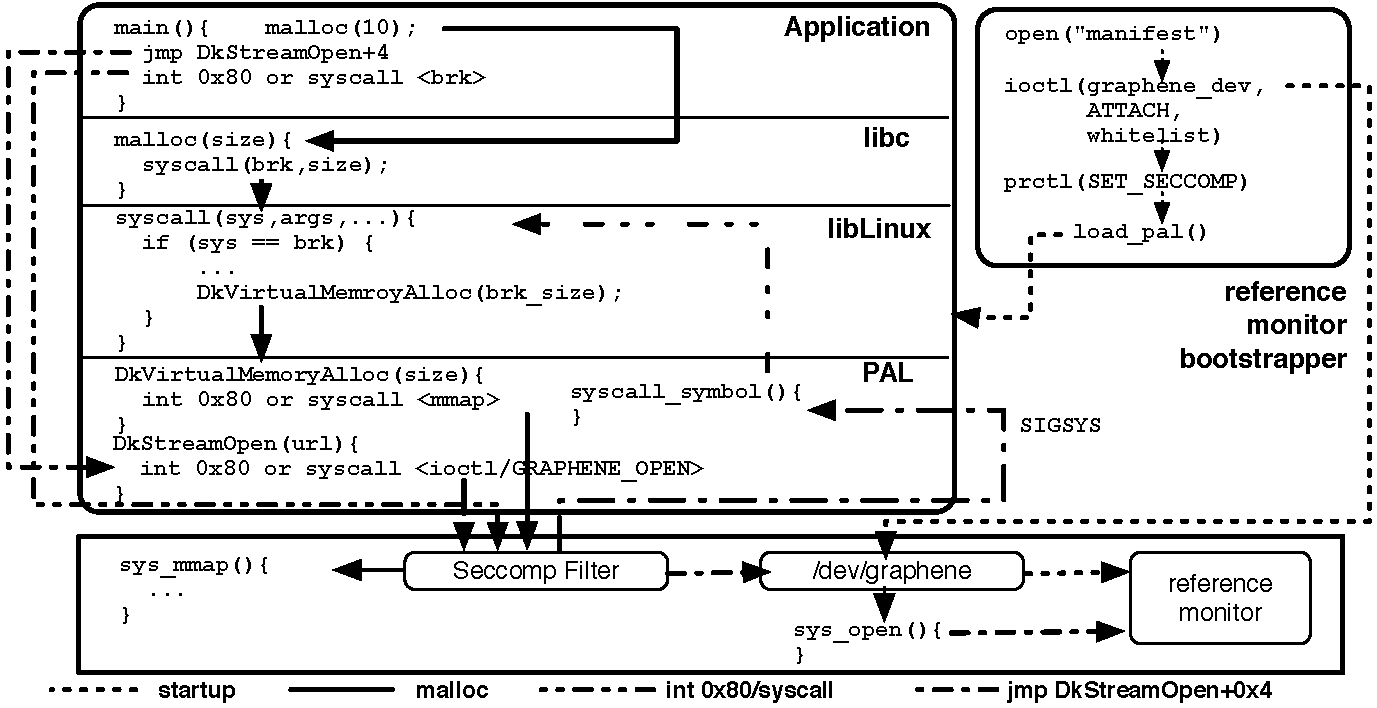
\includegraphics[width=\linewidth]{syscall-restriction.pdf}
%\footnotesize
%\caption[System call restriction approach in sysname{}]
%{System call restriction approach. The reference monitor loads policies into the LSM at startup.  A \graphene{} application requests OS services in three different ways. 
%In the normal case (first line of {\tt main}), {\tt malloc} is invoked causing the invocation of {\tt brk} ({\tt libLinux}) and {\tt mmap} in the \pal{}. In the second line, the application jumps to an address in \pal{}, which is permissible.
%Files are accessed through {\tt ioctl} to {\tt /dev/graphene} and checked by reference monitor.
%The third line invokes {\tt brk} with an {\tt int} instruction, which is redirected to the {\tt libLinux} function.}
%\label{fig:graphene:syscall-restriction}
%\end{figure}



\issuedone{1.3.d}{Extend the discussion of \seccomp{} filter}
\graphene{} restricts the host system calls 
using a \seccomp{} %(SECure COMPuting)
filter~\cite{seccomp}, a feature introduced in Linux 2.6.12.
% a recent Linux system call filtering mechanism, called 
A \seccomp{} filter allows a Linux process to install an immutable Berkeley Packet Filter (BPF) program
that specifies allowed system calls, as well as specifies
the consequence of invoking certain system calls, such as creating a \code{ptrace} event or raising a \code{SIGSYS} signal.
The BPF grammar is rich enough to filter scalar argument values,
such as only permitting specific opcodes for \syscall{ioctl},
as well as filter certain register values, such as blocking system calls from program counters (i.e., \code{RIP} register values) outside of the Linux PAL.
%This feature is particularly salient in the case of {\tt ioctl},
%where the \pal{} uses 5 out of over 400 opcodes for our bulk IPC module and sandbox creation;
%our BPF rules will block any other {\tt ioctl} opcode.
The current \seccomp{} filter installed by the Linux PAL contains \seccomplines{} lines of straightforward BPF macros.  %Experiments show that adding more precise argument checks has no significant impact on system call latency.
Once a \seccomp{} filter is installed in a process,
the filter intermediates
every system calls from the process and its future children, and guarantees the processes can never bypass the restriction.
The Linux PAL uses \code{SIGSYS} signals to capture rejected system calls,
and can either terminate the whole application or
redirect the system call to \thelibos{}.
The consecutive steps of system call redirection are described in Section~\ref{sec:libos:syscall-redirection}.



Developing a \seccomp{} filter presents several technical challenges.
First, a filter must restrict consecutive \picoprocs{}
to install a new filter the reverts the system call restriction.
%A \seccomp{} filter is installed using the \syscall{prctl} system call, so
Blocking the \syscall{prctl} system call in a \seccomp{} filter will prevent further installation of \seccomp{} filters.
Second, the BPF grammar can only filter certain values or ranges of a register.
The filter needs to
ensure that only the Linux PAL can invoke system calls;
however,
for satisfying the dynamic loading behavior of \thehostabi{},
the Linux PAL
is built as a shared library loaded at an address randomized by the Linux ASLR (Address Space Layout Randomization) feature.
If a filter only permits a specific range of program counters,
a child \picoproc{}
will load the Linux PAL at another randomized address,
and the inherited filter will restrict the child \picoproc{} to invoke any system calls.
The Linux PAL introduces a small, initial loader
loaded at a fixed address
within each \picoproc{} and permitted to invoke system calls.
Finally, a \seccomp{} filter
cannot check a string argument, such as a file path for \syscall{open} or a network address for \syscall{bind}.
Checking a string argument requires
involves reading user memory of unknown sizes and string comparison, and the BPF grammar only allows checking an argument arithmetically.
Filtering permitted file paths and network addresses
must rely on a trusted reference monitor (see Section~\ref{sec:linux:security:ref-monitor}).
%In order to avoid the overhead of trapping to the reference monitor on 
%every use of {\tt open}, {\tt stat}, {\tt bind} or {\tt connect} system calls, we instead 
%force picoprocess to only use {\tt ioctl} system call to \graphene{} special device ({\tt /dev/graphene}) as alternative interface these system calls. Direct access to these system calls are banned by seccomp filter.
%extend AppArmor~\cite{apparmor} 
%to enforce file system isolation in the kernel.



The \seccomp{} filter blocks  unauthorized system calls
from anywhere inside a \picoproc{}.
Even if none of the application binaries contains any \assembly{syscall} or \assembly{int \$80} instruction,
a piece of malicious application code can always bypass the Linux PAL
to invoke unauthorized system calls.
The application code can simply
jump to a \assembly{syscall} instruction inside the Linux PAL,
or corrupt a returned address on the current stack to launch a ROP (return-oriented programming) attack.
Even if the Linux PAL is hidden or isolated from the application,
an adversary can always leverage a gadget, a byte sequence that resembles the target instruction, within an executable or a library.
Therefore, the \seccomp{} enforces both program-counter-based 
and argument-based restrictions
to block unauthorized system calls from both the Linux PAL and the rest of \picoproc{}.


%In order to reduce the impact of bugs in the reference monitor,
%the reference monitor itself runs with a \seccomp{} filter, blocking unexpected system calls.


\paragraph{Security implications.}
Using an existing system call restriction mechanism like \seccomp{},
\graphene{} limits the ability of an untrusted application to attack a Linux kernel.
Ideally, since \thelibos{} only requires \thehostabi{},
\graphene{} can adopt a modified Linux kernel
that only exports \palcallnum{} \hostapis{} to each \picoproc{}.
%However, as a usability feature, \graphene{} runs \graphene{} on an unmodified Linux kernel using a Linux PAL to translate among host interfaces.
The \seccomp{} filter instead isolates a \picoproc{} on an unmodified Linux kernel,
with a reduced attack surface 
comparable to only exporting \thehostabi{}.
%The filter only permits \hostsyscallnum{} system calls with specific flags and opcodes
%required by the Linux PAL.
According to the principle of least privilege,
each component or layer in a system should only be granted access to a minimal amount of resources or abstractions
required for performing the expected tasks.
The \seccomp{} filter only permits
a minimal amount of system calls with specific flags and opcodes
required by the Linux PAL,
so an untrusted application
can only trigger
a limited amount of execution paths inside the host Linux kernel.
\graphene{} limits
the ability of an untrusted application to explore
known and unknown vulnerabilities
on any kernel execution paths for servicing one of the blocked system calls.



Although a regular Linux process can also leverage a \seccomp{} filter,
\graphene{} makes a major contribution
to reduce the system call footprint of any large-scale application
to a fixed, small system call profile.
Analysis %of applications and libraries
%in the official Ubuntu repositories
shows that the system call  footprint of a large-scale application such as Apache or MySQL can contain more than 100 system calls.
Since \thelibos{} has absorbed the Linux system call table,
running Apache, MySQL, or any other application in \graphene{} leads to at most \hostsyscallnum{} host system calls.
As a system
running a wide range of applications
can exposes a different partial view of the system call table to each application,
\graphene{}
has a static system call profile for all applications,
allowing OS developers to focus
on testing or analyzing a small portion of execution paths and corner cases
of a Linux kernel.
\citet{sun15unpredictability}
proposes sandboxing an uncertain, potentially-malicious application
in \graphene{}
with an unpredictable \thelibos{} implementation.







\paragraph{Static binaries.}
Besides security purposes,
a \seccomp{} filter provides a compatibility feature
for redirecting hard-coded system calls
in a statically-linked application binary.
\graphene{} leverages the \seccomp{} filter to redirect these leaked system calls
back to \thelibos{}. 
The filter contains BPF rules to check if the program counters
invoking the system calls
are parts of the Linux PAL.
The filter blocks system call invoked outside of the Linux PAL
and delivers a \code{SIGSYS} signal
to the PAL signal handler for redirecting the system calls to \thelibos{}.



\papersubsection{Reference monitor}
\label{sec:linux:security:ref-monitor}

The reference monitor on a Linux host
checks the arguments of host system calls for referencing any sharable host resources.
A host system call like \syscall{open}, \syscall{connect}, or \syscall{bind}
specifies a file system path or a network address
for opening a file or network stream and cannot be filtered by a \seccomp{} filter.
The host kernel trusts the reference monitor
to only permit
a list of sharable resources in a \picoproc{},
based on
rules in a manifest file.
Once the reference monitor has permitted the creation of a file or network stream,
consecutive operations on the stream
such as reading or writing data can be trusted
as long as being mediated by one of the permitted system calls.


\begin{figure}
\centering
\begin{lstlisting}
loader.exec = file:/usr/sbin/apache2        # allow loading executable 
loader.preload_libs = file:/graphene/libLinux.so    # loading libLinux
fs.allow_ro.libc = file:/graphene/libc/     # loading modified libc
fs.allow_ro.mods = file:/usr/lib/apache2/modules/   # loading modules
fs.allow_ro.cond = file:/etc/apache2/       # reading configuration
fs.allow_rw.logs = file:/var/log/apache2/   # writing to logs
fs.allow_ro.http_docs = file:/var/www/      # reading website files
net.allow_bind.httpd = 0.0.0.0:80           # binding to local port 80
net.allow_conn.any = 0.0.0.0:1-65535        # allow any connection
\end{lstlisting}
\caption{A example of a manifest file, containing security rules for the reference monitor to permit accessing sharable resources. The manifest file is for running a Apache http server (without php and other language engines).}
\label{fig:linux:manifest-example}
\end{figure}


The reference monitor enforces simple, white-listing rules
based on security mechanisms
already familiarized by users and developers.
Figure~\ref{fig:linux:manifest-example} shows an example of resource access rules
in a manifest.
First, a manifest lists
the URI prefixes of permitted files or directories
of an application,
similar to an AppArmor profile.
The executable (\code{loader.exec}) and the preloaded \libos{} binaries (\code{loader.preload\_libs})
are permitted for read-only access by default.
The reference monitor
simply compares file URIs against each permitted URI prefix
and checks the access types;
unlike many existing security mechanisms in Linux and similar OSes, such as permission bits, Access Control Lists (ACLs), and SELinux labels,
the reference monitor does not retrieve
security policies from file metadata, but obtains the manifest from an out-of-band channel.


Manifest-based security
simplifies the inspection, authentication, and population
of security policies.
An Android application is deployed with a similar manifest,
listing the accessed files and other resources,
which users approve when installing the application.
Developers can authenticate a security policy by signing the content of a manifest.
Moreover, to run an application, a user can choose among multiple manifest files
with different levels of security privileges.



Network rules in a manifest are similar to {\bf iptables firewall rules} for defending a server or a desktop machine.
A network rule specifies a local or remote address
that the application is permitted to bind or connect a network stream.
A local or remote address
can be an IPv4 or IPv6 address (possible to specify an ``any'' address, i.e., \code{0.0.0.0} or \code{[::1]}), combined with a specific port number or range.
When an application creates a network stream,
the reference monitor checks whether the local and remote addresses
match one of the network rules.







%is implemented using {\tt ioctl} system call to a special device {\tt /dev/graphene}.
%A picoprocess is restricted by seccomp filter~\cite{seccomp} to use any {\tt open} or socket {\tt connect} and {\tt bind} system calls.
%It must use the \graphene{} special device to open or create streams,
%so the file paths or network addresses can be checked against the sandbox rules.
%The kernel module as the driver of the \graphene{} special device can coexist with any LSM such as \emph{AppArmor} or \emph{SELinux}.

The reference monitor on a Linux host
is implemented as a Linux Security Module (LSM) extended from the existing AppArmor module.
AppArmor is the default LSM of most Linux distributions,
and a Linux kernel disallows multiple LSMs (e.g., AppArmor, SELinux) to be effective simultaneously.
\graphene{} instruments
a few security hooks of the AppArmor, to add checks for file system paths
and network addresses.
The security checks of the reference monitor are stackable with other host security mechanisms.
For example, if a manifest lists a root-privileged file and the \graphene{} application runs in a unprivileged process,
existing security checks in a Linux kernel
still blocks the file access even though the reference monitor permits the access.
The drawback of the implementation
is that \graphene{} must run on a modified Linux kernel.
Linux kernels do not support loading LSM as a dynamic kernel module.
\graphene{} only replaces
the AppArmor LSM in a Linux kernel; the rest of the Linux kernel remains unchanged.


A trusted security loader initializes the reference monitor
when launching an application in \graphene{}.
When a user launches an application in \graphene{} from the command line,
the first \picoproc{} begins in a new sandbox.
The security loader
reads the manifest file given by the user,
and submits the sandbox rules to the reference monitor.
The reference monitor exports a miscellaneous device called \code{/dev/graphene}
for the security loader to submit sandbox rules using the \syscall{ioctl} system call.
Once the reference monitor
starts a \picoproc{} in a sandbox, neither the first \picoproc{} nor any consecutive \picoprocs{} spawned in the sandbox can ever escape the sandbox or drop the restrictions on certain resources.


\paragraph{Alternative approaches.}
Other approaches can implement the reference monitor without modifying a Linux kernel, with a trade-off of performance or development simplicity.
An approach is to implement the reference monitor as a trusted process receiving \code{ptrace} events from \graphene{} \picoprocs{}.
Using the \syscall{ptrace} system call, this reference monitor can retrieve user memory from the monitored \picoprocs{},
and block the system calls which request for unpermitted resources.
Unfortunately, intercepting every system calls with \code{ptrace} events introduces significant overhead to \hostapis{};
thus, this approach is not ideal for isolating \graphene{} applications on a Linux host.


Another approach is to translate the resource rules in a manifest file
to AppArmor or iptables rules.
As explained in previous paragraph, the file and network rules in a manifest file are similar to the file lists in an AppArmor profile and the firewall rules enforced by iptables.
Instead of implementing a \graphene{}-specific reference monitor,
\graphene{} can convert a manifest file, either statically or dynamically,
to security rules recognized by AppArmor and iptables.
This approach requires no modification
in a Linux kernel, and can benefit from
existing optimizations of AppArmor and iptable. %these security mechanisms.
\graphene{} leaves the integration with AppArmor and iptables for future work.




\paragraph{Dynamic process-specific isolation.}
A child \picoproc{} may either inherit its parent's sandbox, 
or start in a new sandbox,
by either specifying a flag to \palcall{ProcessCreate} or calling the sandboxing \hostapi{}, \palcall{SandboxSetPolicy}.
A new sandbox may obtain a subset of the original file system view,
but can never request access to new regions of the 
host file system. 
%The restrictive policy enforced on the child will be written in a new manifest file generated by the parent, and the policy will be checked by the reference monitor.
If a child \picoproc{} voluntarily moves itself to a new sandbox
using \palcall{SandboxSetPolicy},
the Linux PAL issue another \syscall{ioctl} call to \code{/dev/graphene}
to dynamically detach
the \picoproc{}
from the parent's sandbox and update sandbox rules. The reference monitor
closes existing RPC streams and prevents RPC stream creation 
across sandboxes.
%among picoprocesses
%that are not in the same sandbox.
%and restricts external connections to remote URIs according to firewall rules in the manifest.
When a process detaches from a sandbox,
the reference monitor effectively splits the original sandbox
by closing any RPC streams that could bridge the two sandboxes.


\begin{comment}
We hasten to note that program counter filtering
is only provided for backwards compatibility, not security.
An attacker can compromise the \pal{}, so system policies are enforced
externally by the reference monitor.


Dynamically redirecting system calls to {\tt libLinux} is 
less efficient than dynamically linking against
the \graphene{} libc or statically compiling {\tt libLinux} into the application.
The overhead of dynamic redirection comes from 
transferring control to the kernel, then back to 
the \pal{}, and then to {\tt libLinux}.
We leave exploration of more efficient alternatives for future work,
such as redirecting the hardware system call table to {\tt libLinux}
on a host system like Dune~\cite{belay12dune},
or dynamically rewriting parts of the static binary~\cite{hunt99detours}.
\end{comment}

%\paragraph{Example.}
%Figure~\ref{fig:graphene:syscall-restriction} illustrates three possible situations. 
%%% An unmodified Linux application is dynamically linked against the 
%%% \graphene{} {\tt libc}, 
%%% which then dynamically links its system calls from {\tt libLinux},
%%% which in turn links in the host kernel ABI from the \pal{}.
%%% The application requests OS functionality in three ways.
%An unmodified application first invokes the {\tt libc} function {\tt malloc}, which issues 
%a {\tt brk} system call to {\tt libLinux}, which requests memory 
%from the host via a {\tt Dk\-Virtual\-Memory\-Alloc} \pal{} call,
%which ultimately issues an {\tt mmap} host system call.
%The {\tt mmap} host system call is allowed by seccomp because it only 
%affects the picoprocess's address space.
%The second line of the application jumps to the \pal{} instruction that issues
%an {\tt open} system call.
%From a security perspective, this is permissible,
%as it is isomorphic to \pal{} functionality.
%In practice, this could cause
%corruption of {\tt libLinux} or application data structures,
%but the only harm is to the application itself. 
%Because this system call involves the file system, the reference monitor LSM first checks if the file to be opened is included in the sandbox definition (manifest) before allowing  the {\tt open} system call in the kernel.  
%Finally, the application uses inline assembly to issue a {\tt brk} system call;
%%in an attempt to obtain I/O port privilege; 
%because this system call was not issued by the \pal{},
%seccomp will redirect this call back to the \pal{},
%which then calls the {\tt libLinux} implementation.


Sandbox creation in \graphene{} can provide
more options than virtualization, to reflect the security policy of applications at any timing,
in the granularity of picoprocess. 
A picoprocess can voluntarily detach itself from the current sandbox, dropping its privileges,
after finishing security-sensitive operations.
If a picoprocess decides one of its children is not trustworthy, it may also start the child under a restricted manifest,
or promptly shut down RPC streams to stop sharing OS states.
The picoprocess that moves to a separate sandbox will have a restrictive view of the filesystem, and no coordination with the previous sandboxes.
Section~\ref{sec:eval:graphene} describes an experiment that improves security isolation of Apache http server without sacrificing functionality.



%We add a \pal{} call which
%permits a picoprocess to request that it be moved into a new sandbox.
%This call, as well as file system path checks, are implemented
%as extensions to the  AppArmor LSM~\cite{apparmor}.
%%We modify \sandboxmodlines{} lines in the
%%to implement this call,
%The new sandbox call closes any open stream handles that cross sandbox boundaries;
%mediate path lookups;
%and create a new broadcast stream for multi-process
% coordination (\S\ref{sec:graphene:namespaces:blocks}).
%%The reference monitor also interposes on this call so that it can 
%%mediate future stream creation.

%To securely apply seccomp filtering we leveraged the fact that all
%\graphene{} processes have the same parent and also the new
%{\tt NO\_NEW\_PRIVS} bit introduced for Linux processes starting kernel
%version 3.5. This bit can be set by any process, is inherited across
%{\tt fork}, {\tt clone}, and {\tt execve}, and cannot be unset by
%children processes. Thus, we set the {\tt NO\_NEW\_PRIVS} bit in the initial
%\graphene{} process and apply seccomp filters allowing only system calls
%with corresponding functions in the \pal{}. As a result all \graphene{}
%processes will inherit the filters and cannot relax or bypass it.



%which reduces the kernel
%system call API surface to user-level processes. This mechanism allows
%a process to specify a whitelist filter for system calls, which is
%implemented as a Berkeley Packet Filter (BPF) program. The invocation
%of a disallowed system call causes the application to throw a {\tt SIGSYS}
%signal, which can be caught by a registered handler provided by the
%application. In \graphene{} we registered this handler at the \pal{}.


%\graphene{} applications rely on an OS loaded as a library to request
%system services. As most of traditional applications, \graphene{}
%processes do not normally issue system calls directly: they invoke
%wrapper functions from a \graphene{}-compliant version of libc, which
%allows for portability, security (parameters are limited and checked)
%and easiness of programming. However, while standard libc functions
%directly invoke the kernel system call themselves, our modified
%version of libc wrappers invoke functions from another library which
%represents the OS, libLinux (Figure \ref{fig:graphene:syscall-restriction}). A
%\graphene{} application can access all necessary system functionality
%through libLinux, which invokes corresponding system call functions at
%the \pal{}, also loaded as a library with a
%\graphene{} process. The \pal{} is the layer responsible for directly
%invoking system calls at the kernel. As discussed in \S\ref{sec:graphene:impl} the \pal{} provides \graphene{} applications with a
%subset of the kernel system call interface.\graphene{} applications rely
%on an OS loaded as a library to request system services.
%
%Even though we expect most of \graphene{} applications to leverage libc
%wrappers, we need to address applications that need to invoke system
%calls directly. Applications might need to bypass a library such as
%libc because some needed wrappers are not provided (there are no
%wrappers in libc for module and NUMA related system calls), or the
%wrapper does not meet the programmer’s needs. \graphene{} applications
%that need to perform direct invocation of system calls run unmodified
%as long as the system calls invoked are provided by the libos{l{}. We
%do not consider this a security violation; even though the application
%would be risking not functioning according to the libosaradigm for
%bypassing the \pal{}, all potential damage would be confined in the
%misbehaving application itself.  However, we do not allow the direct
%invocation of a system call that does not have a corresponding
%function in the libosnd \pal{}. In Figure \ref{fig:graphene:syscall-restriction}
%we illustrate these three situations. We have a \graphene{} application
%loaded with three libraries: a \graphene{}-compliant libc, libLinux
%representing the library OS with functions for a selected number of
%system calls, and the \pal{} which actually invokes host kernel system
%calls. The illustrated application requests three different types of
%OS functionality. It first invokes a function from libc, then it
%directly invokes a system call whose functionality is provided by the
%\pal{}, and third it attempts to directly invoke a system call not
%present in the \pal{}, which is not allowed by \graphene{}.

%We enforce system call restriction by leveraging seccomp Linux system
%call filtering mechanism~\cite{seccomp}, which reduces the kernel
%system call API surface to user-level processes. This mechanism allows
%a process to specify a whitelist filter for system calls, which is
%implemented as a Berkeley Packet Filter (BPF) program. The invocation
%of a disallowed system call causes the application to throw a {\tt SIGSYS}
%signal, which can be caught by a registered handler provided by the
%application. In \graphene{} we registered this handler at the \pal{}.
%
%To securely apply seccomp filtering we leveraged the fact that all
%\graphene{} processes have the same parent and also the new
%{\tt NO\_NEW\_PRIVS} bit introduced for Linux processes starting kernel
%version 3.5. This bit can be set by any process, is inherited across
%{\tt fork}, {\tt clone}, and {\tt execve}, and cannot be unset by
%children processes. Thus, we set the {\tt NO\_NEW\_PRIVS} bit in the initial
%\graphene{} process and apply seccomp filters allowing only system calls
%with corresponding functions in the \pal{}. As a result all \graphene{}
%processes will inherit the filters and cannot relax or bypass it.


%\begin{figure}
%\begin{centering}
%\includegraphics[width=2.0in\textwidth]{figures/syscall_restriction.png}
%\footnotesize
%\caption{System call restriction approach. \graphene{} application requesting OS services. The {\tt printf} function is handled by a wrapper function at our modified version of libc., which invoked a corresponding syscall function at libLinux, the library OS.This function invokes a system call function at the \pal{}, which actually invokes kernel system calls. The application also directly invokes two system calls and the last invocation is prohibited.
%\label{fig:syscall_restriction}
%\end{centering}
%\end{figure}

%\end{comment}

\chapter{System Overview}
\label{chap:overview}

\makeatletter
\def\input@path{{overview/}}
\makeatother
\graphicspath{{overview/figures/}}

%\section{Introduction}
%\label{sec:dcache:introduction}

Operating System kernels commonly cache file system data and metadata in 
a virtual file system (VFS) layer, which abstracts low-level file systems into a common API, 
such as POSIX.  
This caching layer has become a ubiquitous optimization
to hide access latency for 
persistent storage technologies, such as a local disk.
%whether a local disk or a network appliance, 
%have substantially higher access latencies than RAM,
%this caching layer 
%% SOSP Space - kind of quacking on
%% Caching
%% the file system directory hierarchy is particularly important because 
%% low-level file systems often spread this information across 
%% multiple disk sectors.
%% If an application wanted to open a single file on a system without a directory cache, 
%% most low-level file systems would issue numerous disk reads to locate the file and check the permissions
%% on the file and its parent directories;
%% a directory cache can commonly avoid these reads.
The directory cache is not exclusively a performance optimization; it also simplifies 
the implementation of {\tt mount}-ing multiple file systems, 
consistent file handle behavior,
and advanced security 
models, such as SELinux~\citep{selinux}.



%\fixmedp{Be charitable to developers, make our strong claims positively (we are really smarties) rather than calling them dummies}


%% Many observation shows that, in most systems, operations to storage are often
%% dominated by hierarchical structure traversal,
%% and fetching metadata of objects.\fixmetsai{references here}~\citep{duchamp94nfs}
%% In many file systems, traversal and metadata fetching
%% create random access patterns,
%% which are slower than sequential access patterns
%% on many storage media, e.g. magnetic disks.

% dp: I think this is getting down in the weeds.  We need to make the case for the work 
%     more strongly and generally first
%% Directory entry cache, a.k.a \dcache{},
%% is an important optimization in Linux kernels
%% to reduce storage operations for traversal and metadata fetching.
%% The design of \dcache{} is comparable to \vnode{} in BSD and \dnlc{} in Solaris.
%% \dcache{}, as well as \vnode{} and \dnlc{},
%% can be explained as a file system layer that
%% responds to requests on a cache hit,
%% but passes requests down to lower-leveled file systems on a cache miss~\citep{zadok06, skinner93}.

%\fixmedp{F1: Maybe thread together an argument about why no one would have tried a one-hop lookup before?}


%\marginpar{\scriptsize \textcolor{blue}{ Michael, I think the high-order bits are mostly right on Fig~\ref{fig:dcache:lookup-frac},
%but these number may change a bit as we refine the measurement}}

\begin{figure}[t]
\scriptsize
\centering
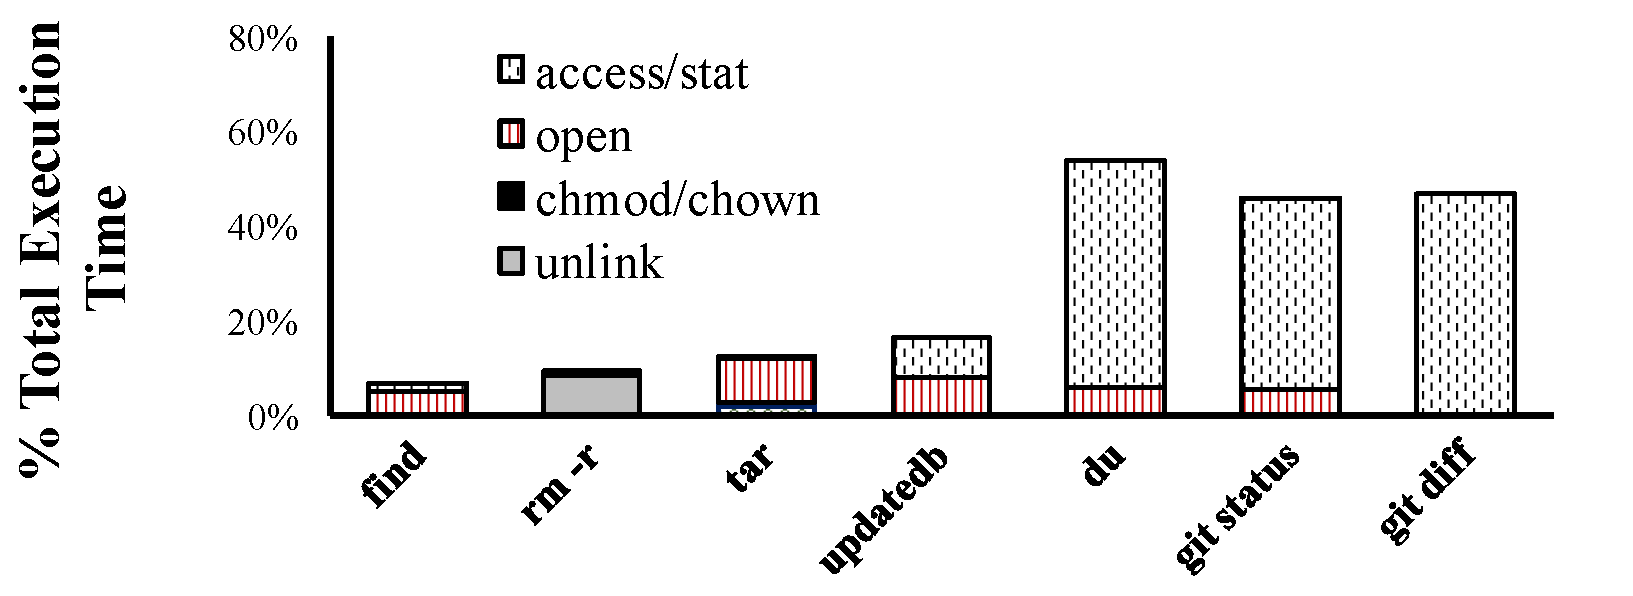
\includegraphics[width=5in]{dcache/plots/syscall-percentage.pdf} \\
\caption[Fraction of execution time on path-based system calls.]
{Fraction of execution time in several common utilities spent
executing path-based system calls with a warm cache, as measured with ftrace.}
\label{fig:dcache:lookup-frac}
%\vspace{-10pt}
\end{figure}

%\fixmedp{Please check these \% against time.  I think git diff is too high.  git status seems ok.}

Directory caches are essential for good application performance.
%Unix was designed such that ``(almost) everything is a file'',
%thus even accesses to in-memory file systems, device files, FIFOs and domain sockets
%first pass through the directory cache.
%In other words, 
Many common system calls must operate on file paths,
which require a directory cache lookup.
For instance, between 10--20\% of all system calls in the iBench system call traces do a path lookup~\citep{filenotafile}. 
Figure~\ref{fig:dcache:lookup-frac} lists the fraction of total execution time
%, as well as system time, 
several common command-line applications spend executing path-based system calls
(more details on these applications and the test machine in \S\ref{sec:dcache:eval}).
We note that these system calls include work other than path lookup,
and that these numbers include some instrumentation overhead;
% are coarse measurements that include  and work than path lookup;
%, and includes some time 
%for synchronous I/O (e.g., during {\tt rename}) as well as non-path tasks (e.g., creating 
%a file handle as part of {\tt open});
nonetheless, in all cases except {\tt rm},
the system call times and counts are dominated by
{\tt stat} and {\tt open}, for which 
%can be serviced from cache and for which 
path lookup is a significant component of execution time.
For these applications, path-based system calls account for 6--54\% of total execution time.
%and 25--77\% of system time.  
This implies that
lowering path lookup latency is
 one of the  biggest 
opportunities for a kernel to improve these applications' execution time.




\begin{figure}[t!]
\centering
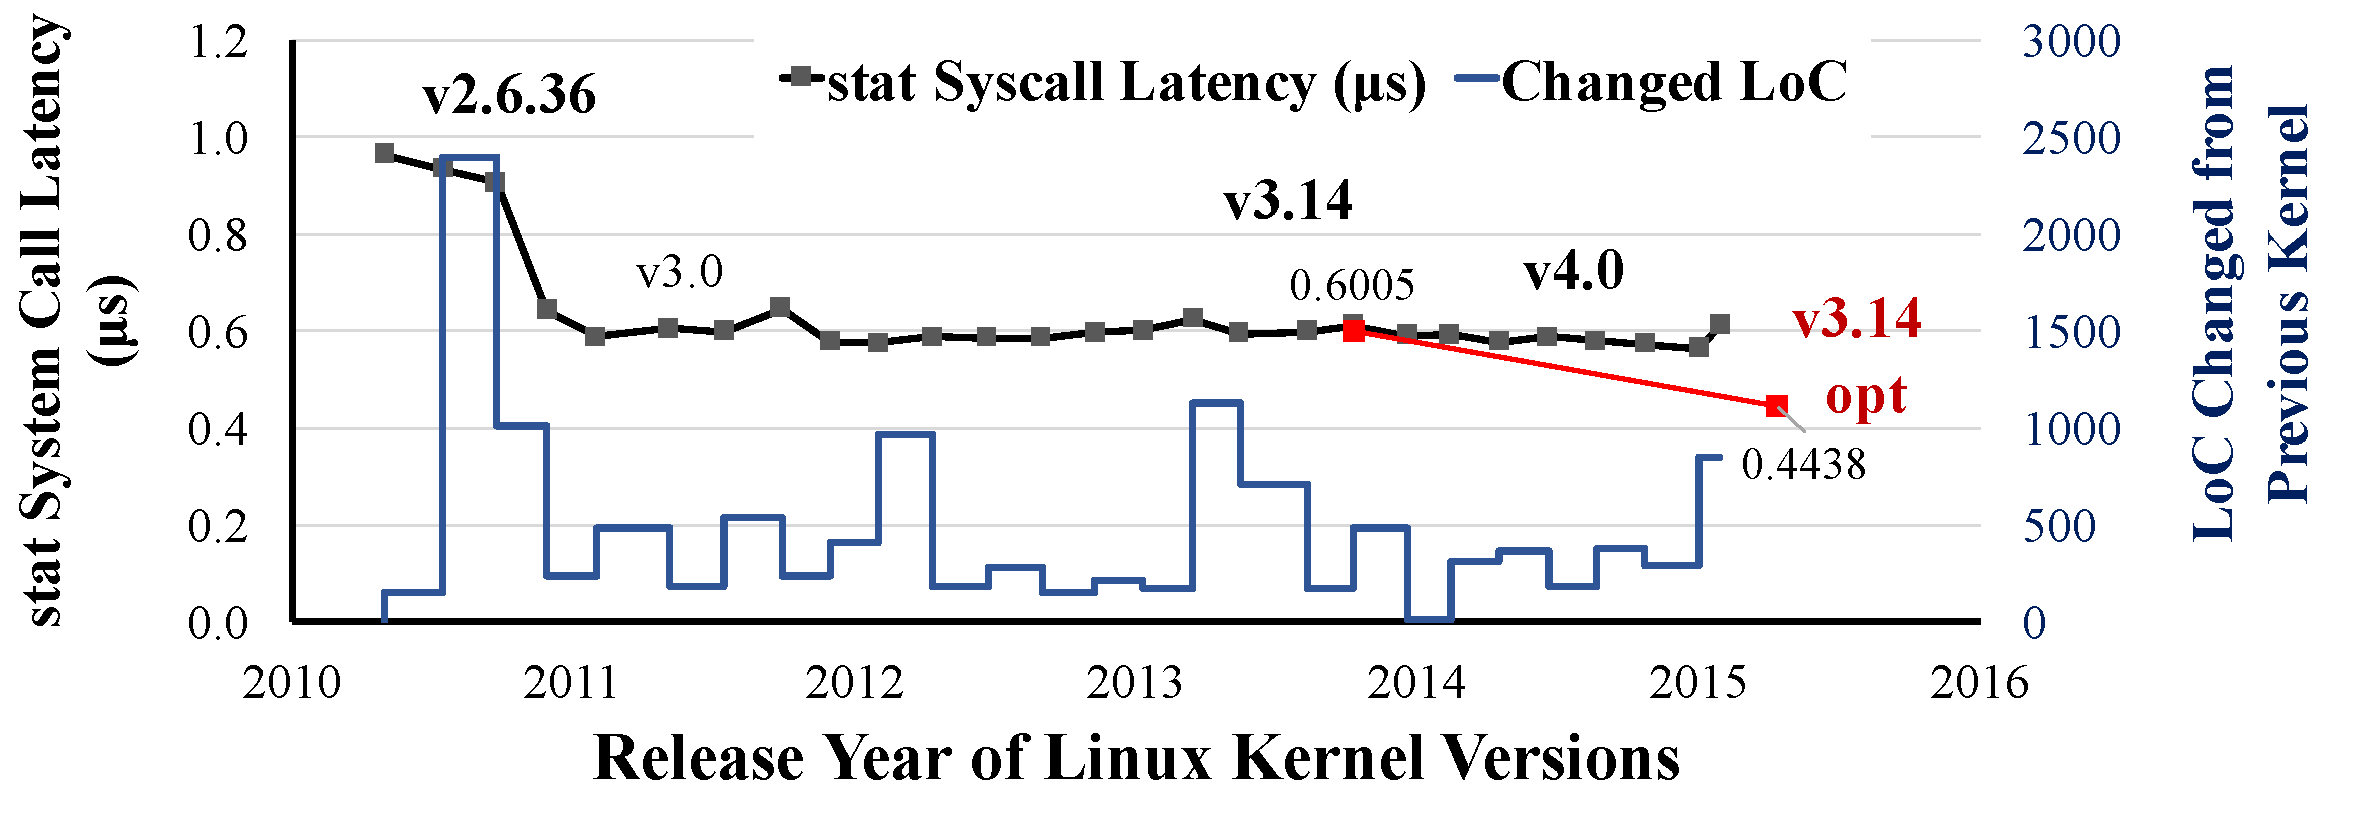
\includegraphics[width=6in]{dcache/plots/latency-by-version.pdf}
\footnotesize
\caption[Lantecy of {\tt stat} system call over years.]
{Latency of {\tt stat} system call with a long path {\tt XXX/YYY/ZZZ/AAA/BBB/CCC/DDD/FFF} on Linux over four years (lower is better), as well as the churn within the directory cache code (all insertions in {\tt dcache.c}, {\tt dcache.h}, {\tt namei.c}, {\tt namei.h} and {\tt namespace.c}). 
%Our optimizations significantly improve performance that has otherwise plateaued, despite significant ongoing developer effort.  
Our optimized \linuxver{} kernel 
further reduces {\tt stat} system call latency by \statspeedup{}\%.}
%\vspace{-15pt}
\label{fig:dcache:by-version}
\end{figure}


%\fixmedp{Add more evidence of lookup importance here: For instance, fraction of lookup time in file-related syscalls, or total lookup time in applications bound on file lookup latency.  }
Unfortunately, even directory cache hits are costly---0.3--1.1 \us{} for a {\tt stat} on our test Linux system, compared to only .04 $\mu$s for a {\tt getppid} and 0.3 \us{} for a 4 KB {\tt pread}. 
%\fixmetsai{Don, check this, I think read will be a better example, getppid is too trivial.}
This issue is taken particularly seriously in the Linux kernel community, which has 
made substantial revisions and increasingly elaborate optimizations to reduce the hit cost
of its directory cache, such as removing locks from the read path or replacing lock ordering with deadlock avoidance in a retry loop~\citep{corbet09jls,dcache-rcu}.
Figure~\ref{fig:dcache:by-version} plots directory cache hit latency against  lines of directory cache code changed 
over several versions of Linux, using a path-to-inode lookup \microbench{} on the test system described
in \S~\ref{sec:dcache:eval}.
These efforts have improved hit latency by 47\% from 2011 to 2013, but have plateaued
for the last three years.
%\fixmedp{if time, filter irrelevant changes from code deltas}
%at the cost of substantial developer effort.
%This latency appears to have plateaued 

The root of the problem is that the POSIX path permission semantics
seemingly require work that is linear in the number of path components,
and severely limit the kernel developer's implementation options.
%The root of this problem is that current directory cache
%designs reflect a straightforward implementation of the POSIX specification,
%which would seemingly require work that is linear in the number of path components.
For instance, in order to open file {\tt /\fnone{}/\fntwo{}/\fnthree{}} 
%for reading, 
one must have search permission
to parent directories {\tt /}, {\tt /\fnone{}}, and {\tt /\fnone{}/\fntwo{}},
as well as permission to access file {\tt \fnthree{}}.
The Linux implementation %of this specification is straightforward, 
simply walks the directory
tree top-down to check permissions.  
Unfortunately, when the critical path is dominated by 
walking a pointer-based data structure, 
including memory barriers on some architectures for multi-core consistency, 
modern CPUs end up stalling on hard-to-prefetch loads.
Moreover, because so many Linux features are built around this behavior, such as Linux Security Modules (LSMs)~\citep{wright+lsm},
namespaces, and mount aliases, it is not clear that any data-structural enhancements
are possible without breaking backward-compatibility with other Linux kernel features.
A priori, it is not obvious that a faster lookup algorithm, such as a single hash table lookup, 
can meet these API specifications and kernel-internal requirements; to our knowledge,
no one has tried previously.

%This paper proposes a decomposition of the directory cache, which allows
%most lookup operations to execute with a single hash table lookup (\S\ref{sec:dcache:dcache}),
%as well as optimizations to reduce the miss rate based on information that is {\em already in the cache}, but not used effectively (\S\ref{sec:dcache:readdir}).
%Our design maintains compatibility (\S\ref{sec:dcache:generalize}) through 
%several essential insights, including 
%how to separate the indexing of paths from checking parent permissions,
%and how to effectively and safely memoize the results of access control checks.


%% This paper proposes several new ways to organize a directory cache, which can yield 
%% substantial performance improvements over the current state of the art.
%% %This paper demonstrates that, despite this developer effort, there is still a substantial 
%% %missed opportunity hiding behind historical, intuitive, but not fundamental design choices.
%% Most of the Linux directory cache design reflects a straightforward implementation of the POSIX 
%% specification. %, with a division of labor that is suitable for mainstream file systems.

%This paper presents an alternative directory cache organization, which 
%improves performance by separating logical tasks, such as separating path indexing from permission checking; yet the design is sufficient to retain compatibility with POSIX.
%In the case of path lookup, 
%this paper demonstrates how 
%a per-component tree walk can be replaced with a single hash table lookup (\S\ref{sec:dcache:dcache}).
% without violating POSIX compliance.

%Our optimizations improve the performance of frequent lookup operations, but 
%introduce several costs, described in \S\ref{sec:dcache:dcache} and measured in \S\ref{sec:dcache:eval},
%which  we believe are acceptable and a net improvement for applications.
%First, these optimizations slow down infrequent modifications to the directory hierarchy, such as {\tt rename}, {\tt chmod},
% and {\tt chown} of a directory. 
%However, these slower operations
%account for less than .01\% of the system calls in the iBench traces~\citep{filenotafile}.
%Second,  the memory overheads of the dcache are increased.
%%(45\% per \dentry{}, as well as some  in our prototype).
%%(\fixmedp{XX MB} in our tests).  
%Third, lookup has a 
%probability of error from signature collisions that can be adjusted to be negligible
%%($2^{-141}$ in our configuration), 
%and within acceptable thresholds widely used by data deduplication systems~\citep{Debnath:2010:CSU:1855840.1855856, Srinivasan:2012:ILI:2208461.2208485, Quinlan:2002:VNA:645371.651321, Zhu:2008:ADB:1364813.1364831}.
%%, as well as how to remove
%%all memory barriers from the lookup path (\S\ref{sec:dcache:update}).
%In the micro-benchmark of Figure~\ref{fig:dcache:by-version}, our directory cache 
%optimizations improve lookup latency by 
%%revisions improve latency of accessing a long path
%%by 
%\statspeedup{}\% over unmodified Linux.
%%Our design addresses other missed
%%opportunities, such as identifying new opportunities to reduce the miss rate
%%through caching directory completeness.
%%\fixmedp{Do we want to highlight LoC?  3K is more than anything in the graph} \fixmetsai{Probably just mention in the evaluation. It's a metric that we should provide, but it's not awfully interesting.}
%%The total lines of code changed are fewer than 3,000 out of \fixmedp{XX}.
%%\fixmedp{Can we get 
%%, yet changes fewer than 3,000 lines of code.

%% SOSP cut - kind of long-winded
\begin{comment}
This paper rethinks current Linux directory cache design choices in light of the following goals:
\begin{compactitem}
\item {\bf Minimize the cost of a cache hit.} (\S\ref{sec:dcache:dcache}).
This means maximizing the benefit of temporal locality for frequent operations,
while pushing extra work of consistency maintenance onto less frequent, already-expensive operations.
%such as handling cache miss or updating massive metadata,
%in order to improve very frequent operations.
\item {\bf Maintain legacy compatibility.} (\S\ref{sec:dcache:generalize}).  Unix path semantics are complex, required by applications, file systems, and security modules, frustrating otherwise straightforward optimizations.  However tempting it may be to redesign path behavior to facilitate caching, path operations must exhibit the same behavior, with lower latency.
\item {\bf Never miss the same request twice in quick succession.} (\S\ref{sec:dcache:readdir}).  A number of less-frequent operations, such as reading a directory or secure temporary file creation, always miss in the cache {\em even if enough information is in cache to satisfy the operation.}  
%Of course, infrequent accesses should still be subject to a cache replacement policy, such as LRU.
\end{compactitem}
%Although directory caches must implement more complex semantics than a hardware memory cache,
%these principles should seem familiar to the reader with a basic architecture background.
%sadly, the Linux directory cache design violates all three.
\end{comment}

%This paper introduces several techniques to improve the performance of a directory cache,
%This paper explains several practical directory cache optimizations,
This paper demonstrates that these techniques improve performance for applications that use the directory cache heavily,
and the harm is minimal to applications that do not benefit.
%and that the worst case \microbench{} is only 12\% slower within \fixmedp{XX}\% of unmodified Linux.
%Each optimization we describe improves performance in isolation, and all can be combined.
%These optimizations change very few lines of code, and are backward-compatible with 
%legacy applications.  
%These changes are encapsulated in the VFS---individual file systems do not have to change their code.
%This paper describes a  prototype of these improvements implemented in Linux \linuxver{}.
%\S~\ref{sec:dcache:background} explains that the directory cache structure of Mac OS X, FreeBSD, and Solaris 
%are sufficiently similar that these principles should generalize.
%we compare and contrast Linux's directory cache
%with Mac OS X, FreeBSD, and Solaris in \S\ref{sec:dcache:background}, and explain inline how each
%optimization could be generalized to these other OS kernels.





%% \item {\bf Modularization and stackability}:
%% Any changes or optimizations must be implemented as modules inside Linux's VFS,
%% and can be stacked on top of the original design or any future optimizations. 
%% \item {\bf Backward compatibility}:
%% Any changes or optimizations must maintain least requirement of modifying any
%% file systems.
%% \item {\bf Generalization to other OSes}: Any changes or optimizations must be portable to other OSes with reasonable effort and change of design.




%% \dcache{} is proven to be effective on improving storage performance.
%% Experiments shows that,
%% in a Linux 3.x kernel, a \dcache{} with a xxx\% hit rate can speed up
%% metadata lookup and fetching time by xxx times.
%% \fixmetsai{experiment result, Linux version, and fs specs here}
%% However, we observed that Linux maintainers have made
%% constant and non-trivial efforts to improve \dcache{} in the Linux kernel.
%% We studied all \dcache{}-related source files in the Linux kernel Git repository,
%% and discovered that maintainers have committed
%% on average xxx revisions per source files.

%% We tested metadata lookup time on primary \dcache{}-related revisions.
%% Most changes on \dcache{} system only create xxx\%-xxx\% speed-up
%% than their predecessor.
%% \fixmetsai{result and graph here}.
%% Moreover, improvement to \dcache{} is still work-in-progress
%% for Linux maintainers.
%% \fixmetsai{reference to threads for latest dcache discussions}. 
%% All the evidences show that,
%% despite of significant reduction of storage operations,
%% efficiency of \dcache{} system internally still remains as a concern.

%% We argue that the design of \dcache{} needs to be carefully re-examined,
%% to fundamentally identify any missed opportunities that
%% improve value of \dcache{}.
%% At a high level, most optimization works for \dcache{} are focused on
%% improving ``how to cache'',
%% but we want to also lay eyes on ``what to cache'',
%% to ensure any valuable information returned from file systems
%% be captured by \dcache{} system.

%The contributions of this paper are as follows:
%\begin{compactitem}
%\item A performance analysis of the costs of path lookup and the opportunities
%to improve cache hit latency.
%\item A directory cache design that improves path lookup latency with a combination of techniques, including:
%  \begin{compactitem}
%  \item Indexing the directory cache by full path, reducing average-case lookup from linear to constant in the number of path components.
%  \item A Prefix Check Cache (PCC) that separates permission checking from path caching.  The PCC memoizes permission checks, and is compatible with LSMs~\citep{wright+lsm}.
%  \item Reducing the cost of checking for hash bucket collisions with path signatures.
%  \end{compactitem}
%\item Identifying opportunities to leverage metadata the kernel already has to reduce miss rates, such as tracking whether a directory is completely in cache.
%\item Carefully addressing numerous, subtle edge cases that would frustrate rote application of these techniques, such as integration with symbolic links and Linux namespaces.
%\item A thorough evaluation of these optimizations.  For instance, our optimizations improve throughput
%of the Dovecot IMAP server by up to \dovecotspeedup\% and latency of 
%updatedb by up to \updatedbspeedup{}\%.
%%git version control system by up to 25\%.
%
%\end{compactitem}

\papersection{\Thehostabi{}}
\label{sec:overview:host}

\issuedone{1.1.b}{Describe \thehostabi{} specification}
The development of \graphene{} starts with defining a simple host ABI (application binary interface) called \thehostabi{},
containing only OS abstractions essential to target applications.
%and is easily ported to different platforms.
%and minimal specifications for the host OSes and hardware.
%The host ABI is a new boundary between OSes (or hypervisors) and applications.
\Thehostabi{} separates
the implementation of an existing system API (application programming interfaces), which determines the compatibility against applications,
from hardware abstraction features, such as file systems, network stacks, and device drivers. 
\graphene{} moves the system API components
to a \libos{} in the userspace and reimplements the functionality using \thehostabi{}.
To port \graphene{} to a new host OS or hardware,
OS developers only have to implement \thehostabi{} on the target host system API,
%to new host OSes and hardware,
instead of paying a tremendous cost to translate the whole system API specification. Figure~\ref{fig:overview:porting} illustrates the porting process of \graphene{}.



%The host ABI separates the low-level, hardware management features, from the idiosyncrasy of system interface. 
%\graphene{} moves the upper layer of OS components,
%including the system calls and namespaces, into an library OS,
%leaving \thehostabi{} 
%as a narrowed interface to the host OSes and hardware.
%The host ABI intends to minimize the development effort on each host OS or hardware
%to mitigate the interface distinctions,
%to simply porting the OS abstractions defined in \thehostabi{}.


\begin{figure}[t!]
\centering
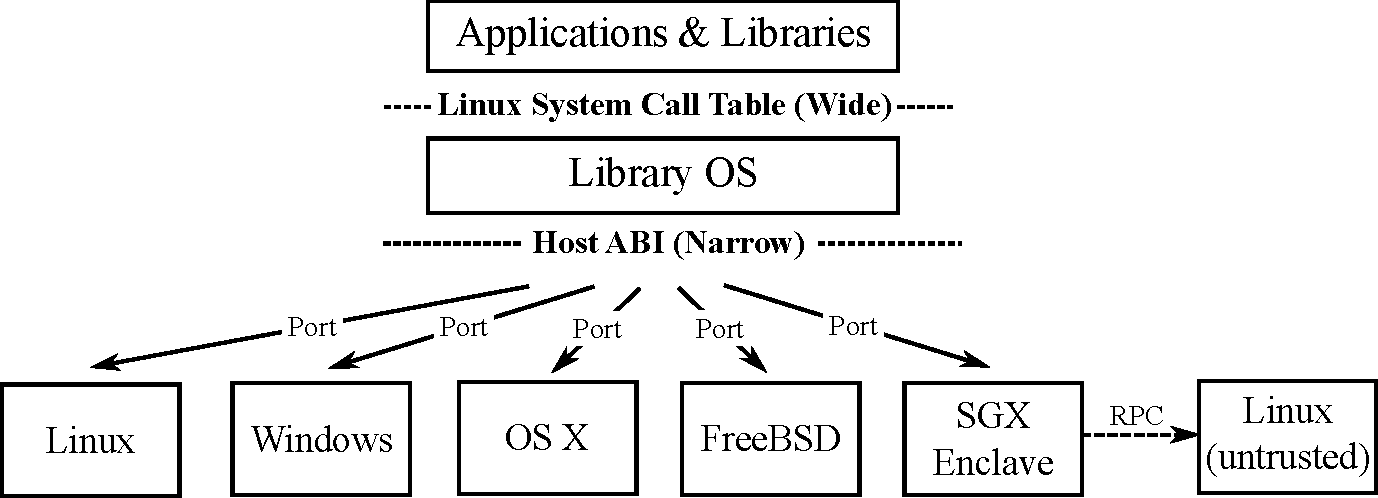
\includegraphics[width=30em]{porting.pdf}
\caption{Porting model of \graphene{}.}
%\vspace{-.1in}
\label{fig:overview:porting}
\end{figure}



\papersubsection{Platform Adaption Layers (PALs)}
\label{sec:overview:host:pal}


For each host OS or hardware, \graphene{} uses
a thin library called a {\bf platform translation layer (PAL)}
to translate among host interfaces.
%is loaded below the library OS, to translate each functions in \thehostabi{} to native system interfaces.
The main purpose of a PAL is to mitigate the semantic gap
between \thehostabi{} and
native host system APIs.
%The effort of PAL development is per host OS, whereas the library OS implementation is reusable on every hosts. %The simplicity of \thehostabi{} can be also estimated by the effort of implementing a PAL for each host.
By implementing a PAL on a new host OS or hardware,
users can reuse
the same \libos{} to run the same collection of unmodified Linux applications.
%To keep the porting effort low,
%the development of a PAL must be straightforward
%for average OS developers.
%to achieve with limited efforts.
%Based on the principle of porting simplicity, PAL development must be straightforward
%for average developers.







%The host ABI is defined for the simplicity of porting, as well as the sufficiency for implementing a library OS compatible to Linux.
%First of all, the number of host functions included in \thehostabi{}
%is much smaller than the number of system calls in a commodity OS such as Linux. 
\graphene{} currently contains PAL implementations for several popular OSes,
including Linux, \win{}, \osx{}, and FreeBSD.
%and \sgx{} with an untrusted Linux kernel.
Most of these OSes provide a POSIX-like system API similar to \thehostabi{}.
Due to the similarity, translating most of \thehostabi{} to one of the system APIs
are straightforward for average OS developers.
\Thehostabi{} is also much smaller than the actual POSIX API, making it extremely portable.



A part of \thehostabi{} may be challenging to port
on an OS,
due to unexpected system assumptions made by the OS.
For instance, \win{} does not support
fine-grained memory deallocation for de-privileged applications.
To implement system calls like \syscall{munmap} and \syscall{mprotect},
\graphene{} needs host ABIs to
deallocate or protect virtual memory pages at page granularity.
%A workaround is to change memory mappings at the physical page level,
%but will require running the \win{} PAL with root permissions.
%This type of porting challenges
%tends to be results of design decisions or assumptions made by OS developers.
%A \libos{} can potentially design
%different emulation strategies
%to compensate missing host abstractions.
A few host abstractions such as a bulk IPC feature are
optional to the host ABI;
if a host OS does not support these abstractions,
the \libos{} must fall back to alternatives. 

%In our experience, the development of a PAL is around ten thousand lines of code.

%For each port, the amount of code written for implementing \thehostabi{} is at the order of magnitude of thousands of lines of code, which is much more manageable than implementing a flat translation layer for system interfaces.


\begin{comment}
Based on the experience in \graphene{},
it is hard to ensure the portability of \thehostabi{} on every potential hosts.
%even a host ABI specialized for simplicity cannot guarantee to be portable on every hosts.
A host may simply lacks the functionality
for implementing a \hostapi{}.
The assumption is, maintaining the compatibility of \thehostabi{} poses a much less challenge than maintaining the whole system API.
Besides, the library OS may flexibly switch among emulation strategies
to compensate the absence of certain host abstraction.
As an example,
bulk IPC is optional in \thehostabi{} since its first definition,
due to the expectation
that implementing the feature may not be feasible on some hosts.
If bulk IPC is not available,
the library OS can fall back to RPC-based IPC, with a reasonable amount of performance penalty.
In the worst case, if there is no emulation strategies
to compensate for the absence of a \hostapi{},
user can predict the affected applications and avoid running these applications
on specific hosts. 
%at least users can predict whether an application will be affected and thus cannot run on certain hosts.
\end{comment}


%For a host OS that does not support ELF binaries, the PAL must follow the binary format which the host OS accepts, such as the Portable Executable (PE) format on \win{}.
%The PAL is the only layer in the user space which cannot be reused
%across different hosts. Besides the PAL, all of the other binaries in the user space are fully reusable, including the library OS, the supporting libraries, and the application executable.



%The host abstractions map to several common system calls in a commodity OS.
%For example, \funcname{StreamRead} and \funcname{StreamWrite} can directly map to the POSIX functions \funcname{pread} and \funcname{pwrite}, which are available in most OSes including Linux, BSD, \osx{}, and \win{}.
%More than half of the functions in \thehostabi{} can be counted toward this category.
%The rest of the host abstractions are either specific to Linux
%(e.g., TLS support),
%or belong to the POSIX functions that are not shared with commodity OSes
%(e.g., \funcname{mmap} on \win{}).
%The PAL emulates these host abstractions, using existing system interfaces available on the host OS, unless the software emulation is fundamentally impossible (e.g., restricted by the system interfaces), or too expensive (e.g., high overhead from copying data).



\papersubsection{Definitions and design principles}
 

\graphene{} defines \palcallnum{} calls in \thehostabi{} (also called \hostapis{}),
with a set of host abstractions
sufficient for \libos{} development.
%The host ABI defines the interaction between the library OS and a specific host.
%The \graphene{} library OS can be deployed on any ``host'' where \thehostabi{} has been ported.
This thesis defines
a {\bf host} of \thehostabi{}
to be an OS or hypervisor
which contains enough OS functionality for running a standalone application or virtual machine.
Most of the host targets in \graphene{}
are monolithic OSes,
including Linux, \win{}, \osx{}, and FreeBSD.
%which has defined a massive system API for programmability.
A monolithic OS 
usually contains a massive amount of system APIs,
which is sufficient for
implementing \thehostabi{}.


A special example of a host
is an \sgx{} (Software Guard Extensions) enclaves~\cite{intelsgx},
which
restricts OS functionality for security reasons.
The restrictions on \sgx{}
are results of a strong threat model
which distrusts any OS features except ones that are virtualized by the CPUs or migrated into enclaves.
The only way to obtain any missing OS features such as storage or networking
is to request through RPC (remote procedure call).
Requesting untrusted OS services through RPC also introduces new security threats that application developers tend not to anticipate~\cite{checkoway13iago,osdi16scone}.
Due to all the compatibility and security challenges discussed above,
this thesis uses \sgx{} as a representative example of a host
with unusual assumptions (e.g., threat models) and restrictions
compared to a monolithic OS.

%An innovative hardware abstraction like \sgx{} (software guard extensions)
%imposes unique assumptions and restrictions
%on a commodity OS,
%%creates a special host on top of Linux or \win{},
%%with unique interfaces and specifications regarding the host OSes.
%and thus creates a special host above the OS.

%If an OS has mutated or tweaked the interface for a hardware platform,
%such as an \sgx{} enclave 
%running on an untrusted Linux kernel,
%the combination of the OS (Linux) and the hardware platform (\sgx{}) is considered a specialized host.
%Especially, the \sgx{} port of \thehostabi{} faces several unique challenges,
%which will be discussed in Chapter~\ref{chap:sgx}.


\begin{comment}
%\fixme{each sentense should be a paragraph; starting the 2nd sentence}
\fixmedp{start with a strong opening stating the rationale}
The host ABI of \graphene{}
define functions needed from a host, in order to implement the library OS for reusing applications.
%to reuse an application and all its supporting libraries, including the \graphene{} library OS.
Each host of \graphene{} contains an OS and a hardware platform, either of which causes compatibility issues for running unmodified applications.
OS developers can port the library OS to a new host,
by simply reimplementing the narrowed host ABIs using abstractions available on the host.
%a new host platform.
%For each host which requires the compatibility for unmodified Linux applications, one only has to implement the narrowed host ABIs,
%instead of reimplementing the bloated, ``legacy'' system interfaces
%needed by the applications.
By implementing \thehostabi{}, OS developers skip the painful process of rebuilding the whole system interfaces of a commercial OS such as Linux.
The host ABIs strictly decouples the porting effort on the hosts from the compatibility feature for applications.
%The host ABIs decouple the OS development in the host and the implementation of compatibility for the existing Linux application.
What \thehostabi{} exposes is a simplified extended machine,
similar to a para-virtualization interface, capable of running the library OS as a lightweight virtual machine. % with compatibility against Linux applications.
%on which another layer of virtualization (i.e., the library OS) can be built to reproduce the compatibility for Linux.
\end{comment}


\begin{comment}
Two design principles drive the definition of \thehostabi{}s:
{\em simplicity} (i.e., easy to port on any hosts)
and {\em sufficiency} (i.e., containing enough OS functions for implementing a library OS).
The process of deciding \thehostabi{}s is comparable to
finding a ``pinch point'' within a OS implementation,
which can conveniently mediate a significant portion of OS execution paths for managing hardware abstractions.
%The two principles drive the development of \thehostabi{}s,
%The whole development of the \graphene{} library
%must be disciplined
%on extending \thehostabi{}s only when it is strongly required.
%of restraining extensions to \thehostabi{}s unless absolutely necessary.
The two principles
determine the soundness of the \graphene{} approach to improving compatibility
for any hosts.
\end{comment}


%%The host ABI is defined with partitioning in mind.
%\Thehostabi{} 
%determines a boundary which partitions several upper-level OS components, %, such as system calls and namespaces,
%into a library OS,
%%, as a dynamically-linked library which can be deployed
%%to various hosts.
%%The rationale behind the partitioning is based on the fact that not every OS component is equally important to compatibility, for applications which need to be ported across hosts.
%%When an OS is extended for a new hardware,
%%these OS components usually remain unchanged, or are predominantly reused.
%%Partitioning
%%into a library OS further guards these 
%in order to isolate the host idiosyncrasy. % on specific hardware. %any potential changes for adopting new hardware.
%%Similar isolation
%%exists in traditional OSes, but without partitioning:
%The strategy
%is also used in OSes:
%An example is the Linux virtual file system (VFS), an internal interface
%which encapsulates operations of file system drivers.
%%On the other hand,
%%drivers (e.g., drivers for file systems, block devices, or network cards)
%%and architecture-specific instructions
%%stay encapsulated in the host OS.
%%in the Linux kernels are usually encapsulated under a virtualized, in-kernel interface (e.g., the Linux virtual file system),
%%to simplify the development of the rest of the kernel.
%Similar to VFS,
%\thehostabi{} is intended
%to be a more ubiquitous interface,
%which encapsulates
%any host-specific behavior and semantic
%inside the host OS.
%%for encapsulating both OS and hardware idiosyncrasy on a wide range on hosts.
%%declares a ubiquitous system interface, to encapsulate both OS and hardware abstractions
%%for the library OS.




\Thehostabi{} shares several characteristics with a virtual hardware interface
exported by a hypervisor.
A generic, backward-compatible
virtual hardware interface
%a set of generic, virtual hardware,
%which the VM can control with the same drivers.
allows an unmodified OS kernel to run inside a virtual machine as on the bare metal.
%by exporting interfaces close to commodity hardware.
%To avoid additional porting effort, the virtual hardware are close to the typical commodity hardware.
%For instance, a virtual hardware interface
%usually includes a virtual NIC (network interface controller),
%such as the virtualized E1000 interfaces
%available in VMware workstation or QEMU.
%As a result, \thehostabi{} contains the
%typical OS features and interfaces, similar to the API of early UNIX systems.
The key difference between
a virtual hardware interface
and \thehostabi{}
is that \thehostabi{} does not target reusing a whole, unmodified OS kernel as a guest.
Instead, 
\thehostabi{} contains higher-level abstractions such as files and network sockets
to ensure portability on most host OSes.
The concept
of defining \thehostabi{}
with a customized guest OS (i.e., a \libos{}) running atop \thehostabi{} is similar to para-virtualization.
%\thehostabi{} expects the \libos{}
%to be rewritten and
%customized for \thehostabi{},
%similar to a 
%para-virtualizated VM.
%Compared to an actual para-virtualized VM,
A para-virtualized VM defines hypercalls as interfaces between a guest OS and a hypervisor.
Furthermore, \thehostabi{} avoids duplication of OS components
such as scheduler, page fault handler, file systems, and network stacks
between the host and \libos{}.
%Another difference is that \thehostabi{} is called by normal function calls, whereas para-virtualization relies on hypercalls.
To compare a VM and a \libos{} on a spectrum,
a VM reuses a whole OS on a wide, backward-compatible virtual hardware interface
whereas a \libos{} implements only system API components on a simplified host ABI.

The following paragraphs discuss the key design principles of \thehostabi{},
including porting simplicity, sufficiency for \libos{} development, and ease of migration.

\paragraph{Porting simplicity.}
%To reduce porting effort
%\thehostabi{}
%must be simple to port on a host OS or hardware.
To reduce porting efforts,
\graphene{} defines \thehostabi{}
using two strategies:
first, \graphene{} significantly reduces both the size and complexity of host OS features
that OS developers have to implement.
Effectively, \graphene{} avoids duplicated OS features and handling rare corner cases
on \thehostabi{}.
%The development of \graphene{} disciplinarily avoiding adding any functions to \thehostabi{},
%unless the library OS cannot internally implement an OS feature.
Second, the definition of \thehostabi{}
imitates common system APIs in a POSIX-like monolithic OS,
to directly translate most calls to
a few similar host abstractions.
%existing system calls or system library functions
%on each host.
%include functions which can be directly mapped to OS functions exported by the host.
%%the likelihood of finding similar features on the host, to be translated to functions in \thehostabi{}.
%The assumption that such a strategy is possible
%is based on
%the observation that
%%similarity of system interfaces is common among most OSes.
%similar OS functions, especially UNIX-style APIs,
%tend to commonly exist in most OSes.
%, to reduce the learning curve for programming applications.
For instance,
the stream APIs in \thehostabi{}, such as \palcall{StreamRead} and \palcall{StreamWrite}
are similar to
system calls like \syscall{read} and \syscall{write} exist on Linux, BSD, and POSIX API,
or \syscall{ReadFile} and \syscall{WriteFile}
on \win{}.
%with similar functionality and semantics.
%and 
%looks similar to \syscall{ReadFile} in \win{}, except the data types.
%The definition of \thehostabi{}
%is based on observations of the system interfaces in some of the important hosts,
%including Linux system calls and \win{} API.
%exported by the targeted hosts,
%and defines the functions in \thehostabi{}, to be easily translated to the native system interfaces.
%The host ABI is essentially a subset of the common features from every potential hosts.
%We expect %\thehostabi{} defined with simplicity in mind
%to be straightforward to port on most hosts,
%Most functions in \thehostabi{} can be easily translated to host system interfaces
%in various styles.
As the rest of this thesis proves, porting \thehostabi{} is straightforward
on most monolithic OSes.

%For example, \thehostabi{} defines \syscall{StreamRead} and \syscall{StreamWrite} for accessing I/O streams, similar to .
%xcept some nuanced details like order of parameters.


% by including OS functions , such as \syscall{FileRead} and \syscall{FileWrite}, similar to the Linux system calls, \syscall{pread} and \syscall{pwrite}.




\begin{comment}
The simplicity of \thehostabi{}s requires retaining a minimalist design of host functions. %, based on typical OS services for managing hardware.
%\graphene{} reduces the host functions
%to the bare minimum.
The host ABIs should only contain operations that
are absolutely necessary for requesting external hardware abstractions.
%A way to simplify \thehostabi{}s is to move host functions into the library OS
%and to replace them with wrappers consisting of other host functions.
Any functions that can be partially or wholly implemented inside the library OS
should be further simplified, or even removed from \thehostabi{}s.
%---in other words, whether \thehostabi{}s can be further reduced.
Moreover, \thehostabi{}s have to be simple enough to implement on
most hosts;
%In the simplest host ABIs, none of the host functions shall be able to internally implement the behavior of another host function,
%or the definition of \thehostabi{}s is further reducible.
that is, \thehostabi{}s should contain only OS functions that are commonly offered on
most hosts.
The host ABIs are close to simplified UNIX interfaces,
such as reading or writing a file or an I/O device as a byte stream,
or creating a virtual memory mapping.
%the most common OS functions
%offered on most of the potential hosts,
For most hosts,
implementing \thehostabi{} should be as straightforward as redirecting the functions to the closest host system calls.
%such as the Linux system calls or the \win{} APIs.
For example, the functionality of \syscall{StreamRead} and \syscall{StreamWrite} in \thehostabi{}s can loosely match with
\syscall{read} and \syscall{write} in Linux,
or \syscall{ReadFile} and \syscall{WriteFile} in \win{}.
%This thesis also evaluates the simplicity of \thehostabi{}s by counting the lines of code used to implement \thehostabi{}s on each host platforms.
Since most OSes have inherited a similar design from UNIX,
it is fair to assume finding
comparable OS functions %host platforms
to \thehostabi{} would be reasonably easy.
%fair to assume that \thehostabi{}s 
\end{comment}



\paragraph{Sufficiency for \libos{} development.}
%\Thehostabi{} defines
%the host abstraction available for a \libos{} to access host hardware abstractions.
To develop a \libos{} with compatibility against a wide range of applications,
\thehostabi{}
%are demonstrated by the fact that
%the exported host functions 
contain any OS abstractions that the \libos{} cannot easily emulate.
%and a full-function library OS is implemented on top of them.
For most hosts,
the host OS abstractions
%can be categorized into five types:
include
process creation, memory management, and I/O (typically, files and network connection)~\cite{dhamdhere2007os-textbook}.
%Besides security and protection,
%the definition of \thehostabi{} is closely related with hardware management,
%and offers the most basic abstractions for each category of OS functions.
%managing specific types of hardware,
%and each contain a few basic abstractions
%which can be expanded into other system interfaces.
%For example, the basic OS functions for memory management include
%allocating (\syscall{VirtMemAlloc}),
%protecting (\syscall{VirtMemProt}),
%and deallocating (\syscall{VirtMemFree}) memory regions. % at certain granularity
%(usually in pages).
%These basic functions can be used to implement other forms of memory allocation,
%such as growing heaps with \syscall{brk}
%or allocating thread-private stacks.
%The definition of the \drawbridge{} host ABI is a hint, for creating a list of host abstractions necessary for the library OS, including streams, memory, threads, and processes. 
%If \thehostabi{}s are insufficient for implementing certain system interfaces, one may extend \thehostabi{}s with the missing functions,
%with the discipline to retain the simplicity of \thehostabi{}s.
%The extension to \thehostabi{}s must be d, to keep the extension minimal, and to avoid adding redundant functions.
%The implementation of the \graphene{} library OS demonstrates that
%\thehostabi{} is sufficient for implementing significant portion of Linux system calls.
For each type of abstractions,
a monolithic OS may define several variants of system APIs with similar functionality.
For instance, Linux provides two system calls, \syscall{mmap} and \syscall{brk}, both for memory allocation in a process.
\syscall{mmap} allocates larger memory regions with page granularity,
whereas \syscall{brk} simply grows a single, continuous heap space for more fine-grained allocation.
Many applications such as GCC~\cite{gcc}
switch among system API variants in case one of them is unavailable on certain OS distributions.
This thesis shows that,
by adopting only the semantics of one of these similar APIs or abstractions, the host OS can stay simple with
the \libos{} emulating the rest of APIs.
For instance, \thehostabi{} includes \syscall{VirtMemAlloc}
as a similar feature as \syscall{mmap},
which is sufficient to emulating both \syscall{mmap} and \syscall{brk}.



\graphene{} defines \thehostabi{} partially based on
\drawbridge{},
a library OS for single-process \win{} applications.
The host ABI of \drawbridge{} 
contains 36 functions,
%demonstrates that its host ABI is sufficient
%for running a library OS in which 99.7\% of code comes from the \win{} 7 source.
%The host ABIs of \drawbridge{} are later extended
%for running a Linux-based library OS called Bascule~\cite{baumann13bascule}.
and several works have ported the host ABI to different hosts,
including \win{}, Linux, Barrelfish, and \sgx{}~\cite{porter11drawbridge,baumann14haven,mssql-on-linux,baumann13bascule}.
%and is capable of running a library OS for single-process, Linux applications, with a few host ABI changes~\cite{baumann13bascule}.
%ill loads and links the rest of application binaries, just like the native Linux loader (i.e., \code{ld.so}).
%\graphene{} takes the high-level definitions of the \drawbridge{} and Bascule host ABIs, and customizes for general-purpose Linux applications and a wider range of hosts. 
Although running \win{} and Linux applications may face
a different set of challenges,
the nature of their APIs is mostly similar, with a few exceptions.
During the development of \graphene{}, developers found the occasions in which
the host ABI of \drawbridge{}
is not sufficient to address Linux-specific challenges
and decide to extend \thehostabi{}.
Section~\ref{sec:overview:host:abi} and Chapter~\ref{chap:abi}
will further discuss the Linux-specific extensions of \thehostabi{}.


\paragraph{Migration.}
The \graphene{} library OS shares several features of VMs, including checkpointing and migrating a running application.
Migrating a process is also the key to emulating copy-on-write forking,
on a host without physical memory sharing (e.g., \sgx{}).
A hypervisor checkpoints and migrates a VM by snapshotting the VM states above a stateless virtual hardware interface. % as a clean boundary for snapshotting the application and OS state.
\Thehostabi{} is also defined to be statelessness,
by ensuring any states in the hosts to be temporary and reproducible to the applications and \libos{}.





\papersubsection{The \hostapis{}}
\label{sec:overview:host:abi}


%\fixmedp{the beginning doesn't capture the whole paragraph.}
%The host ABI shares several common abstractions with production OSes.
%The functions in \thehostabi{}
%define the basic features needed from the hosts, to run the library OS.
%The definition of the host functions
%should be unsurprising to average OS developers,
%making the implementation on a new host to be fairly straightforward.
%The host ABI reflects the common functionality of most OSes, including Linux and \win{}.
%Although the same OS abstractions may be defined
%as different idiosyncratic system interfaces on each host OSes,
%\graphene{} takes into consideration of porting the host functions to either OSes, in the most effortless way possible.





%fixmedp{give more of the background}
Table~\ref{tab:overview:abi} lists the \palcallnum{} calls defined in \thehostabi{}:
%Among these \hostapis{}, 
25 calls are inherited from the \drawbridge{} host ABI,
including functions to managing I/O (e.g., \palcall{StreamOpen}), memory allocation (e.g., \palcall{VirtMemAlloc}), scheduling (e.g., \palcall{ThreadCreate}), and several miscellaneous functions (e.g., \palcall{SystemTimeQuery}).
%Most of the host functions only affect the OS or hardware states
%related to the process itself.
%For example, \syscall{VirtMemAlloc} can only allocate memory in the calling process,
%and cannot affect other processes running in parallel.
%Only I/O streaming functions export states to the host OS, and share states with other processes or library OSes.
14 calls are added by \graphene{}, to implement Linux-specific features.
For example, unlike \win{} or \osx{}, Linux %The host ABI is also complemented with several Linux-specific abstractions, such as
delivers hardware exceptions to a process as signals.
Linux also requires 
the x86-specific segment registers (i.e., FS/GS registers)
to determine the location of thread-local storage (TLS), which can be hard-coded in application binaries by a compilation mode of GCC.
On \win{} or \osx{}, the x86-specific segment registers are mostly ignored, and even frequently reset to eliminate attack vectors.
%The host ABI contains host functions (), which can be directly called from the library OS. \graphene{} shows that \thehostabi{} is sufficient to implementing a large portion of the Linux system calls.
%These functions are not defined in \drawbridge{}, the \win{}-based library OS,
%because these abstractions do not exist in \win{}.
%The \drawbridge{} host ABI does not contain exception delivery because the feature is
%not commonly used in \win{} applications.
%Moreover, the x86 segment registers cannot be modified in \win{}
%because the OS assigns fixed values to these registers
%for the whole execution.
%Although \drawbridge{} excludes these abstractions, Bascule extends \thehostabi{} to include similar functions,
%demonstrating that the extension is indeed necessary.
\graphene{} discovers these abstractions as a necessity for implementing a rich Linux \libos{}.



\begin{table}[htp!]
\centering
\small
\begin{tabular}{|p{.15\textwidth}|p{.33\textwidth}|p{.45\textwidth}|}
\hline
{\bf Abstraction} & {\bf Function Names} & {\bf Description} \\
\hline
\raggedright
Streams & 
\raggedright
{\tt StreamOpen} \newline
{\tt StreamMap} \newline
{\tt StreamFlush} \newline
{\tt StreamSetLen} \newline
{\tt StreamRead} \newline
{\tt StreamWrite} \newline
{\tt StreamWaitforClient} \newline
{\tt StreamAttrQuery} \newline
{\tt StreamAttrQuerybyHandle} \newline
{\tt StreamAttrSetbyHandle} \newline
{\tt StreamDelete}
& 
Opening streams using URIs, with prefixes representing stream types (e.g., \code{file:},\code{tcp:},\code{pipe:}),
as well as common stream operations, including transmission of data, and query to the stream attributes.
\\
\hline
\raggedright
Memory & 
\raggedright
{\tt VirtMemAlloc} \newline
{\tt VirtMemFree} \newline
{\tt VirtMemProtect}
& 
Allocation, deallocation, and protection of a chunk of virtual memory.
\\
\hline
\raggedright
Threads \& scheduling & 
\raggedright
{\tt ThreadCreate} \newline
{\tt ThreadExit} \newline
{\tt ThreadDelayExecution} \newline
{\tt ThreadYieldExecution} \newline
{\tt SemaphoreCreate} \newline
{\tt SemaphoreRelease} \newline
{\tt EventCreate} \newline
{\tt EventSet} \newline
{\tt HandlesWaitAny}
&
Creation and termination of threads; 
Using scheduling primitives, including suspension, semaphores, events, and pollable IO events.
\\
\hline
\raggedright
Process & 
\raggedright
{\tt ProcessCreate} \newline
{\tt ProcessExit}
& 
Creating or terminate a process with a library OS instance.
\\
\hline
\raggedright
Mis\-cel\-la\-ne\-ous & 
\raggedright
{\tt SystemTimeQuery} \newline
{\tt RandomBitsRead}
& 
Querying system time, and random number generation.
\\
\hline
\raggedright
Exceptions $\dagger$ & 
\raggedright
{\tt SetExceptionHandle} \newline
{\tt ExceptionReturn}
& 
Setting an exception handler, and returning from the handler.
\\
\hline
\raggedright
TLS $\dagger$ & 
\raggedright
{\tt SetSegmentReg}
& 
Setting the \code{FS}/\code{GS} registers.
\\
\hline
\raggedright
Remote Procedure Call $\dagger$ (optional)& 
\raggedright
{\tt StreamSendHandle} \newline
{\tt StreamRecvHandle} \newline
{\tt CreateIpcChannel} \newline
{\tt PhysicalMemoryCommit} \newline
{\tt PhysicalMemoryMap}
& 
Sending opened stream handles or physical memory across processes.
\\
\hline
\end{tabular}
\caption{An overview of \thehostabi{} of \graphene{}. The ones marked with the symbol $\dagger$ are introduced in the initial publication of \graphene{}~\cite{tsai14graphene} or later extended for this thesis. The rest are inherited from \drawbridge{}~\cite{porter11drawbridge}.}
\label{tab:overview:abi}
\end{table}

%The interfaces, as part of \thehostabi{}, which access these host abstractions, are ultimately simplified to reduce the porting effort on each host.
%Unlike the system interfaces in the OS, \thehostabi{} does not prioritize backward compatibility. Therefore, \thehostabi{} includes only the minimum interfaces that the library OS needs to interact with the host. The host ABI does not have to include any of  the legacy system interfaces from a production OS, let alone preserving different flavors of system interfaces for backward compatibility.



\graphene{} introduces five calls for 
remote procedure call (RPC) between \libos{} instances
in a multi-process application.
\graphene{} simplifies porting multi-process abstractions
on each host OS
to implementing RPCs.
The basic RPC abstraction is 
a pipe-like RPC stream for message passing between processes.
To improve performance,
%RPC is critical for implementing the coordination of OS states
%across library OS instances.
%The basic form of RPC in \graphene{} is a pipe-like RPC byte stream, which a library OS can simply use to send messages.
%It is a common design choice
%to implement inter-process coordination through message-passing
%instead of shared memory, especially for hardware platforms that do not guarantee memory coherence~\cite{baumann09barrelfish}.
%A problem to the message-passing approach is the significant overheads
%on frequently exchanging distributed OS states.
\thehostabi{} defines an optional, bulk IPC abstraction
to send large chunks of virtual memory
across processes.
%The bulk IPC feature works similarly as sending the memory through RPC streams,
%but is much faster because it avoids copying memory in the host.


%for host platforms that urgently require lowering the RPC overheads.
%Another extension is for
%%\funcname{StreamSendHandle} and \funcname{StreamRecvHandle}
%delegating opened stream handles to another process, through a connecting pipe.
%The feature is similar to sending file descriptors
%through UNIX sockets in Linux, and is used to share opened network sockets with the \syscall{fork}'ed processes.
%%Another RPC abstraction is a bulk IPC channel; a process can use \funcname{PhsyicalMemoryCommit} to commit a large chunk of memory to a bulk IPC channel, which \funcname{PhsyicalMemoryMap} can map into another process, as copy-on-write. The library OS uses bulk IPC as an optimization to \syscall{fork}.
%Despite that either of the RPC primitives
%is not necessary easy to implement on every hosts, the inclusion of these host functions is completely optional, and the library OS can always fall back to the message-passing approach.



%All the host functions are designed to appear as ``stateless''
%as possible to the library OS.
%Being stateless to the library OS means that
%a host function does not preserve any permanent state of certain host abstraction.
%A stateless function can recover
%from disconnection of the library OS, and be reconnected at any timing.
%The host functions can maintain temporary bookkeeping for the convenience of porting,
%but should not assume the bookkeeping states to be permanent.
%The principle of defining all the host functions to be stateless
%is primarily for two purposes:
%{\em migration} and {\em security isolation}.
%For migration, the fact that the library OS can disconnect freely from the host functions simplifies the implementation of the migration feature.
%Migration is also an important foundation to implementing \syscall{fork}, because the cloned process need to receive a snapshot of the parent process.
%For security isolation, 
%a stateless host function is easier to check,
%because the security monitor only has to verify each instance of host function calls,
%instead of tracing multiple host functions over a longer period of time.

%the functions to access each host abstraction must appear \fixmedp{clarify `stateless'} stateless to the host, except for the handles to identify the resources. Each call to the host functions is independent. The arguments given for each call must be always be absolute values, instead of relative values.
%For example, the offset given to \funcname{StreamMap}, \funcname{StreamRead}, and \funcname{StreamWrite} (if the opened handle is a file) are offsets from the beginning of the file, and thus are irrelevant to how many bytes that are previously written or read.
%When enforcing isolation rules, the host OS can check the arguments of each calls to the host functions, independently and atomically.


%A host ABI (application binary interface) has to define the convention of application binaries, including the binary format and the linking procedure, as well as a set of  system interfaces.
%The host ABIs contain a minimal loader which recognizes a basic version of the ELF (Executable and Linkable Format), just enough to compose a binary of the library OS.
%The very initial loading procedure as part of \thehostabi{}s only loads a clean library OS instance.
%Each host of \graphene{} is supposed implement a minimal dynamic loader,
%which can load the \graphene{} library OS binary in ELF.
%The library OS then completes the dynamic loading procedure,
%by directly loading the Linux native dynamic loader (i.e., \code{ld.so}), and indirectly loading the rest of the application binaries.







\papersubsection{Host-enforced security isolation}
\label{sec:overview:host:security}


To target multi-tenant environments, 
\graphene{} enforces strong security isolation between mutually-untrusting applications running on the same host.
The security isolation of \graphene{} is comparable to running each application
in a VM or a container.
Just as a virtual hardware interface isolating each VM,
\thehostabi{} also enforces security isolation between library OS instances.
%according to the trust model of the applications.


On a trusted host OS,
\graphene{} delegates security isolation as a host-level feature.
The library OS and the application must mutually trust each other, due to lack of internal privilege separation in a process.
%The host ABI also separates API implementation
%from security isolation.
%To ensure isolation, each host must restrict access from the applications or the library OS, to any unauthorized host abstractions.
On each host, a reference monitor enforces security isolation policies, by access control on OS abstractions sharable among processes, including files, network sockets, and RPC streams.
%The host-level security isolation is orthogonal to API complexity.
Separating security isolation from API implementation simplifies security checks
for applications that only require
complete protection from other tenants.
%based on monitoring the references to host resources and rejecting authorized resource access.
%to the host abstractions.





%\graphene{} reduces the attack surface exposed to applications
%by restricting access to the host kernel ABI 
%and prevents access to unauthorized system calls, files, byte streams,
%and network addresses with a \emph{reference monitor}.
%The host kernel ABI exported by the \pal{} heavily 
%limits the ability of a \graphene{} application to interact with the rest of the system;
%any external interactions are further mediated by a reference monitor.
%Unlike a typical Linux system, \graphene{} applications cannot interact with shared 
%system daemons or other shared system resources.
%As a result, \graphene{} enforces security isolation similar to running applications in separate VMs---even
%applications that span multiple processes.


In \graphene{},
one or multiple processes of the same application run in a {\bf sandbox}.
Multiple library OS instances coordinate
in a sandbox
to present a unified OS view
to the application.
%As the library OS instances can coordinate shared OS states using simple RPC streams,
The design simplifies the enforcement of security isolation for multi-process abstractions.
\graphene{}
uses the reference monitor to block RPC streams across the sandbox boundary,
stopping applications in different sandboxes from accessing multi-process OS states.
%\graphene{} contributes a multi-process security model 
%based on the abstraction of a \emph{sandbox},
%or a set of mutually trusting processes.
%If a reference monitor exists, the reference monitor permits the processes within the same sandbox to communicate and exchange RPC messages, but disallows cross-sandbox communication.
The current design focuses on security isolation, although we do expect to extend the design for more sophisticated policies
in the future.

\begin{comment}
The only host abstractions that are shared across processes and must be mediated by the host for isolation are files, network sockets, and RPC streams
--- all other allowed host ABI modify only local process state, such as VMAs and threads.
%Thus, the reference monitor need only mediate file access, socket and RPC stream creation.
%an unprivileged daemon
%as well as extensions to the App\-Armor LSM~\cite{apparmor},
%which checks file and socket policies in the kernel.
%, reducing context switching overhead
%and the risk of race conditions~\cite{garfinkel03traps}.
In order for the reference monitor to restrict file access, socket and RPC stream creation,
each application includes a {\em manifest file}~\cite{hunt07rethink},
which describes a {\tt chroot}-like, restricted view of the local 
file system (similar to Plan 9's unioned file system views~\cite{pike90plan9}),
%including read-only shared files,
as well as {\em iptables}-style~\cite{iptablesman} network firewall rules.
To facilitate sharing read-only libraries, a manifest may specify a file system view which combines several different sub-directories of the local file system, and can prevent writing to files or directories.


For example, the \graphene{} reference monitor on the Linux host is implemented using \syscall{ioctl} to a special device (\code{/dev/graphene})~\fixme{a prospective design}.
A process is restricted by the Linux BPF-style system call filter, or the SECCOMP filter~\cite{seccomp}, to use \syscall{open} to access any files, or to \syscall{connect} or \syscall{bind} to any sockets.
It must use the \graphene{} special device to open or create streams, so the file paths or network addresses can be checked against the sandbox rules. The kernel module as the driver of the \graphene{} special device can coexist with any Linux Security Module (LSM), such as AppArmor~\cite{apparmor} or SELinux~\cite{selinux}.


When a new process is launched by the host, it begins execution in a new sandbox.  
Child processes may either inherit their parent's sandbox, or can be started in a separate sandbox---specified by a flag to the host abstractions of process creation.
A parent may specify a subset of its own file system view 
when creating a child, but may not request access to new regions of the host file system. 
%The restrictive policy enforced on the child will be written in a new manifest file generated by the parent, and the policy will be checked by the reference monitor.
The child may also issue an {\tt ioctl} call to 
dynamically detach from the parent's sandbox. The reference monitor prevents byte stream creation across sandboxes.
%among picoprocesses
%that are not in the same sandbox.
%and restricts external connections to remote URIs according to firewall rules in the manifest.
When a process detaches from a sandbox, effectively splitting the sandbox, the host must closes all RPC streams that could bridge the two sandboxes.
\end{comment}



\paragraph{Threat model.}
For most hosts, application trusts the host OSes as well a \libos{} instances in the same processes.
For multiple processes inside a sandbox,
the \liboses{} in these processes
also trust each other.
Applications or \liboses{} are not trusted by the host OSes or processes outside of the sandboxes.
Applications and \liboses{}
can become the adversary to the host OS,
by exploiting vulnerabilities on \thehostabi{}.
%the \graphene{} design reduces the attack surface between the hosts and the library OS instances, to defend against a malicious application.

%On a host with a reference monitor, the host OS and the reference monitor are both trusted, to mediate all system interfaces used to implement \thehostabi{}. The host must check all access to any abstractions with effects outside of a process's internal state, such as an opened file, or a connected network socket.
%Processes inside the same sandbox mutually trust each other. The adversary can run arbitrary code inside of one or more processes within one or more sandboxes.
%The adversary can control all code in its processes, including the library OS and the host-specific PAL.
%{\tt libLinux} and the \pal{}. 
%We also assume a trusted reference monitor process running on the host kernel that 
%launches \graphene{} applications and mediates all system calls with external effects,\fixmedp{define precisely}

%\graphene{} ensures that %The key security property the \graphene{} design upholds is that 
%the adversary cannot interfere with any victim picoprocesses
%in a separate sandbox.  
%The \graphene{} sandbox design ensures strict isolation: 
%if the only shared kernel abstractions are byte streams and files, 
%and the reference monitor ensures
%there is no writable intersection between sandboxes,
%the adversary cannot interfere with any victim picoprocess.


The threat model of \graphene{} on \sgx{}
contains the adversary from other hosts but excludes
the host OS, hypervisor, and any hardware except the CPU from its trusted computing base (TCB).
An untrusted OS or hypervisor
potentially has lots of opportunities to invade applications or VMs,
using Iago attacks~\cite{checkoway13iago}.
The challenges of porting \graphene{} to \sgx{} is not limited to resolving the compatibility issues of enclaves but also defending applications and \liboses{} against untrusted host OSes.







%%% The only processes allowed to run as standard kernel processes (non-\graphene{}) 
%%% are the reference monitor and
%%% system administration utilities that need more kernel interfaces than the \pal{} ABI provides.
%%% Ensuring that a collaborating picoprocess correctly implements
%%% some function (such as receiving a signal),
%%% as well as preventing exploitation of vulnerabilities in picoprocesses
%%% are beyond the scope of this work.

%\graphene{} reduces the system attack surface of the host, but does not change the size of its
%trusted computing base; however, reducing the effective system call table
%size of a picoprocess does facilitate adoption of a smaller host kernel,
%which we leave for future work.


\papersection{The \libos{}}
\label{sec:overview:libos}

This section gives the overview of \graphene{}, a library OS for reusing unmodified Linux applications
on \thehostabi{}.
%Existing library OSes have established reuse of single-process applications~\cite{porter11drawbridge}.
%The library OSes map a target system API, such as the Linux system calls, to abstractions in \thehostabi{}. %The reduction of host interfaces provides portability to various platforms that can translate the interfaces to host APIs or abstractions,
%and a narrower attack surface that developers can more likely reason about.
% and supporting data structures as library functions---mapping
%high-level APIs onto
%a few paravirtual interfaces to the host kernel.
%Recent library OSes improve efficiency over full guest OSes by eliminating duplicated features
%between the guest and host kernel,
%such as the CPU scheduler, or
%eliminating guest-level multiplexing code, as the library OS supports only one application;
%even compiling out unnecessary guest kernel APIs~\cite{unikernels}.
A \libos{} is comparable to a partial, guest OS running in a virtual machine.
However, compared with an actual virtual machine, the \libos{} design of \graphene{} and previous work~\cite{porter11drawbridge,unikernels} eliminates duplicated features between the guest to the host kernel, such as the CPU scheduler or file system drivers, and thus reduces the memory footprint.
%Library OSes have also been proven useful for reusing applications on new hardware platforms, such as \sgx{} enclaves~\cite{baumann14haven}.
%% dp: This sentence seems a little premature
%In recent works, library OSes provide rich OS features for isolated contexts while the host OSes are untrusted

%% Library OSes reduce the memory requirements of running a self-contained,
%% isolated application process
%% %guest \daniela{I would replaced guest by "isolated process or group of processes (a \libos{} instance)''}
%% by orders of magnitude
%% In a cloud computing environment,
%% increasing the number of applications per server has enormous
%% economic benefits.
%% Even on a desktop or portable system, \libos{}es can reduce the overheads
%% of sandboxing untrusted code and running applications
%% designed for another OS.

%Because library OSes execute within a VM \daniela{this phrase does not read good to me because (i) it might imply the picoprocesses need hypervisor support, as misunderstood by reviewer 1 and (ii) you already emphasized the drawbacks of leveraging a VM} or lightweight process ({\em picoprocess}~\cite{xax}),
%library OSes execute with

%% dp: Daniela, great suggestion!  We need to make this situation seem more
%%     like the sky will fall without our help
A principal drawback for prior library OSes is the inability to support multi-process applications. Many existing applications, such as network servers (e.g., Apache) and shell scripts (e.g., GNU makefiles), create multiple processes for performance scalability, fault isolation, and programmer convenience.
%These applications would benefit from the efficiency and security benefits
%of a library OS.
For the efficiency benefits of library OSes to be widely applicable,
especially for unmodified Unix applications,
library OSes must provide commonly-used multi-process abstractions, such as \syscall{fork}, signals, System V IPC message queues and semaphores, sharing file descriptors, and exit notification.
Without sharing memory across processes, the library OS instances must coordinate shared OS states to support multi-process abstractions.
%To support multi-process abstractions, library OSes often have to rely on sharing OS states,
%backed by the hosts' memory sharing features.
For example, \drawbridge{}~\cite{porter11drawbridge} cannot simulate process forking because copy-on-write memory sharing is not a universal OS feature.


\begin{figure}[t!]
\centering
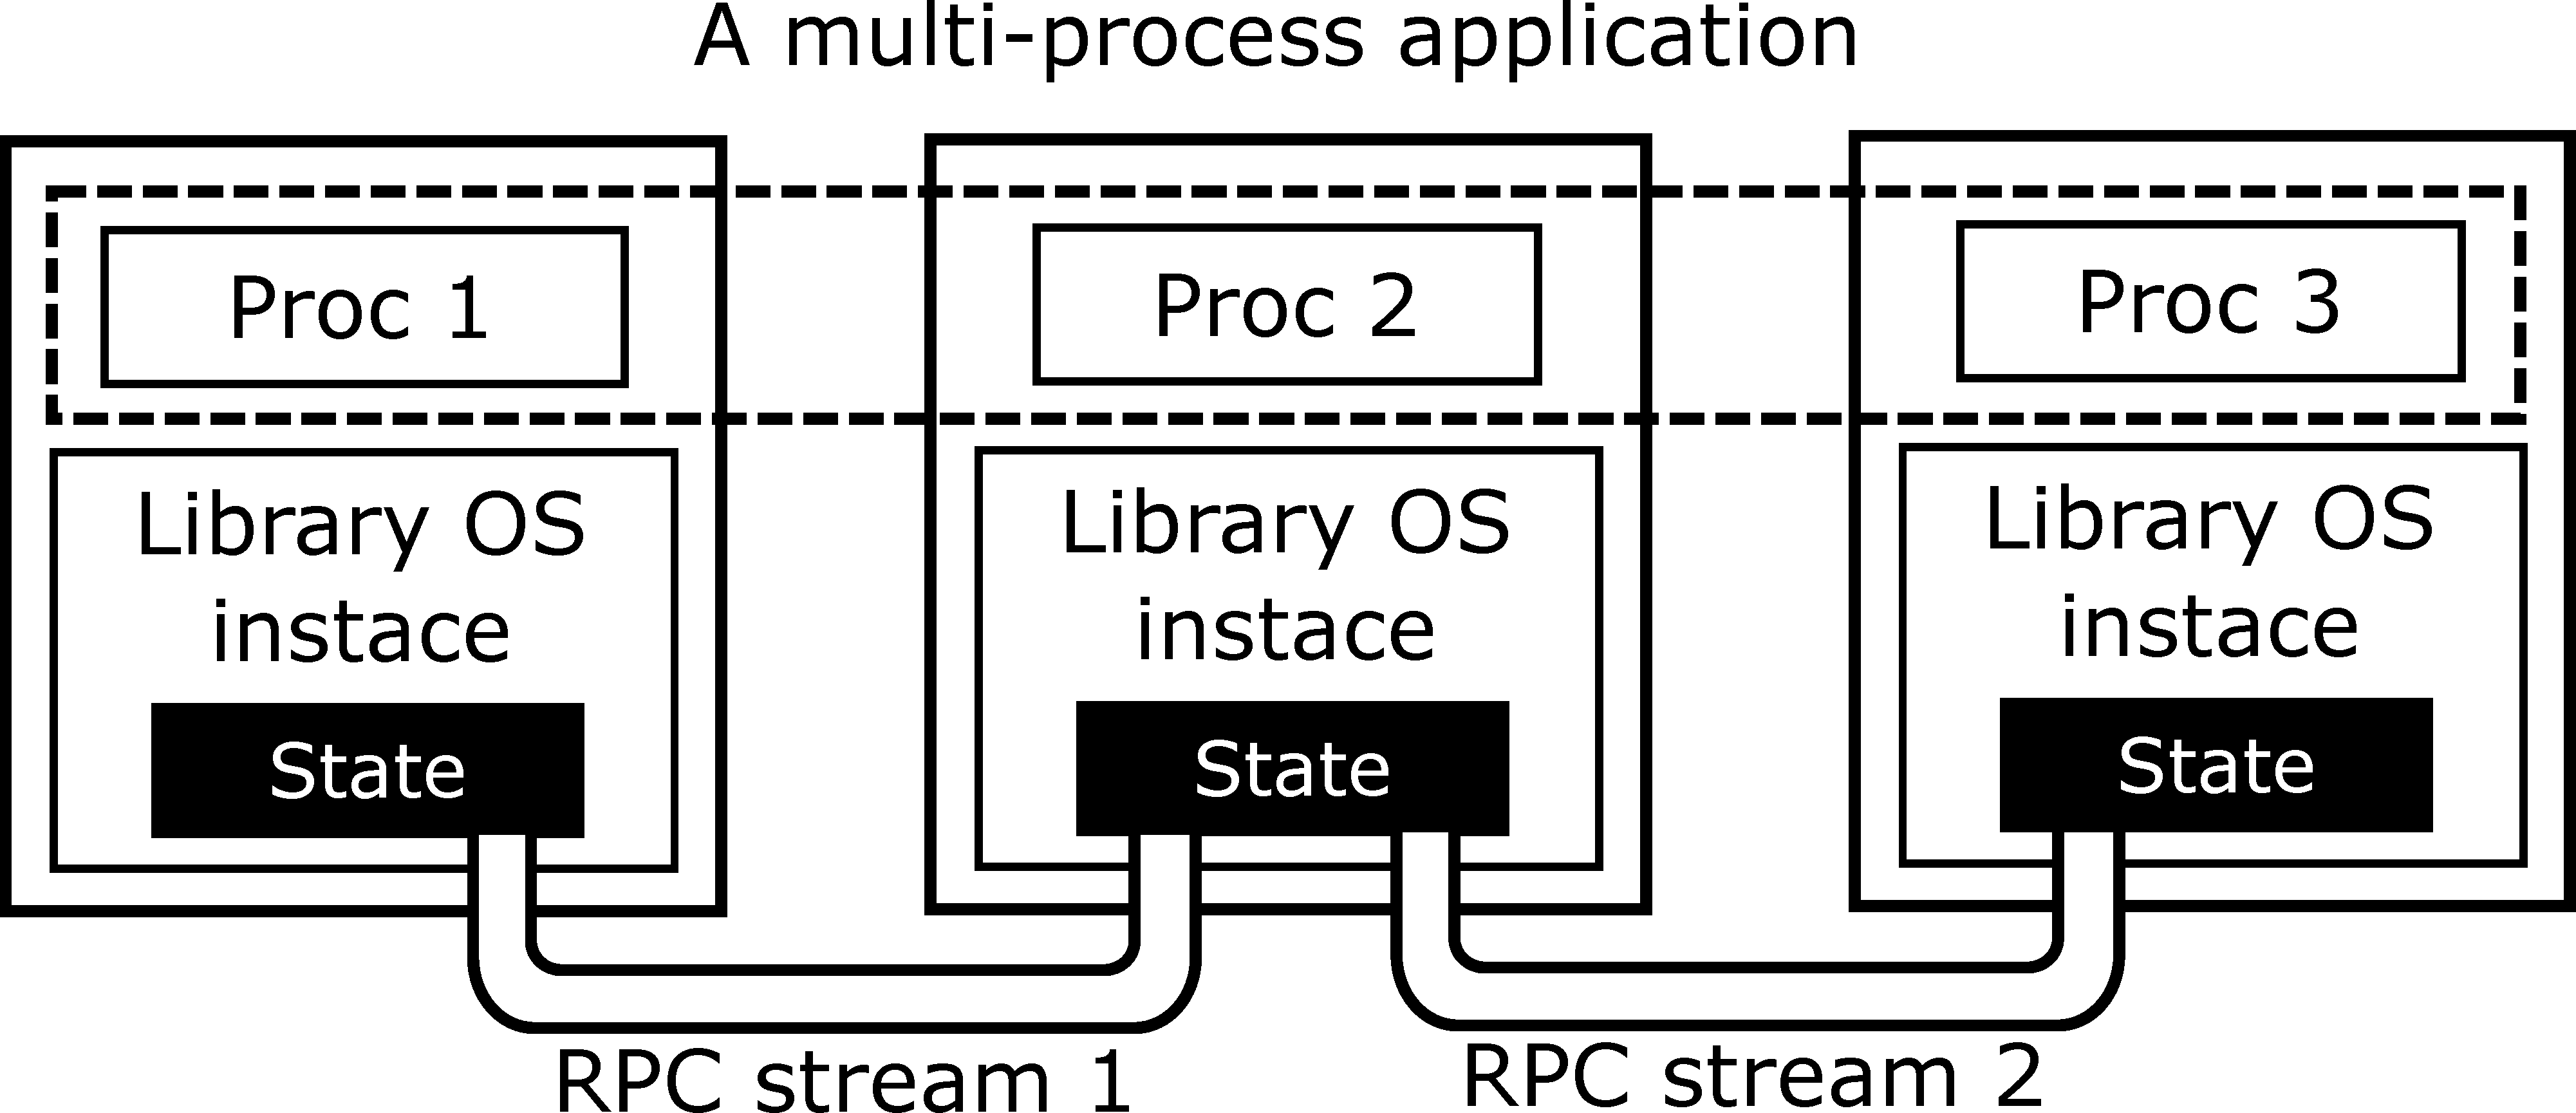
\includegraphics[width=24em]{concept.pdf}
\caption{Multi-process support model of \graphene{} \libos{}. For each process of an application, a \libos{} instance will serve system calls and keep local OS states. States of multi-process abstractions are shared by coordinating over host-provided RPC streams, creating an illusion of running in single OS for the application.}
%\vspace{-.1in}
\label{fig:graphene:concept}
\end{figure}

%{\bf \graphene{}} is a Linux-compatible library OS to run legacy, unmodified Linux applications. 
In \graphene{}, multiple library OS instances collaboratively implement
Linux abstractions, but present single, shared OS view to the application.
\graphene{} instances coordinate states
using message passing over RPC streams.
With a distributed POSIX implementation,
%placement of shared state and messaging complexity are first-order performance concerns.
%%We chose to shift implementation complexity into the library OS
%%in order to uphold simple enforcement of security isolation in the host.
%By coordinating shared states across library OS instances, 
\graphene{} can create an illusion of running in a single OS for multiple processes in an application.

%Previous library OS designs ensured security isolation of independent applications,
%comparable to a VM, by keeping a relatively narrow host ABI.
%We selected the \graphene{}
%design because it strikes a unique balance between
%and robust, flexible security enforcement.
%The \graphene{} design ensures security isolation of
%mutually distrusting, multi-process
%applications on the same host system.
%Essential to this goal is
%minimally expanding the host ABI to support multi-processing,
%as well as leveraging RPCs as a natural point to mediate inter-\picoproc{} communication.
%RPC coordination among \graphene{} instances can be dynamically disconnected, facilitating novel sandboxing
%techniques.  For instance, we develop an Apache web server extension that, upon logging in a given user,
%places the worker process's \libos{} in a sandbox with access to only that user's data.
%We expect more nuanced degrees of trust are possible in future work.

%\graphene{}'s design gives the user and system administrator a high degree of flexibility
%in isolating arbitrary groups of unmodified application processes,
%while upholding the efficiency and host compatibility benefits of recent library OSes.

%\fixmedp{After a complete draft is written, coalesce all goals and make sure they are addressed early on.  We are doing some scatter-shot motivation}


\papersubsection{\Libos{} architecture}
\label{sec:overview:libos:arch}

%Recent library OSes~\cite{porter11drawbridge,unikernels,baumann13bascule,osv}
%are designed for security and efficiency, but are limited to single-process applications.
%The security isolation of \liboses{} derives from 
%limited, explicit data sharing and 
%a narrow host interface.  
A \libos{} typically executes in either a para-virtualized VM~\cite{unikernels,osv}
% \daniela{I would have the use of a VM as a discussion topic in the end of the paper.}, 
or an OS process called a \emph{\picoproc{}}~\cite{porter11drawbridge,baumann13bascule}, with a restricted host ABI.
%The host ABI heavily restrict effects outside of the application's address space
%as a result, applications in a \picoproc{} have very little opportunity to interfere with each other,
%yielding security isolation comparable to a VM.
%The library OS deduplicates features for hardware management in both the guest and host kernels.
\graphene{} executes within a \picoproc{} (Figure~\ref{fig:overview:arch}),
which includes an unmodified application and its supporting libraries, which run alongside a library OS instance.
The \graphene{} \libos{} is implemented over \thehostabi{} designed to expose very generic abstractions that are easy to port on any host OS.
%Although the \graphene{} prototype  host kernel is Linux, 
%we adapt a host ABI from Drawbridge/Bascule,
%which has been previously implemented on \win{}, Hyper-V, and Barrelfish~\cite{porter11drawbridge,baumann13bascule,baumann09barrelfish}.
%The \graphene{} host ABI is
% summarized in Table~\ref{tab:abi} and discussed in more detail in \S\ref{sec:linux:pal}\fixmedp{if not cut...}.  
%which exposes only tens of simple host calls. \daniela{briefly define \picoproc{}: A \picoproc{} is unmodified application code running with a \libos{}.}


\begin{figure}[t]
\centering
\begin{minipage}[b]{1.25in}
\footnotesize
\raggedleft
Linux system calls \\
\graphenesyscallnum{} out of \linuxsyscallnum{}\\
\vspace{0.1in}
Host ABI \\
\palcallnum{} \hostapis{}\\
\vspace{0.2in}
\hostsyscallnum{} Linux system calls
\vspace{0.35in}
\end{minipage}
\hspace{-1.25in}
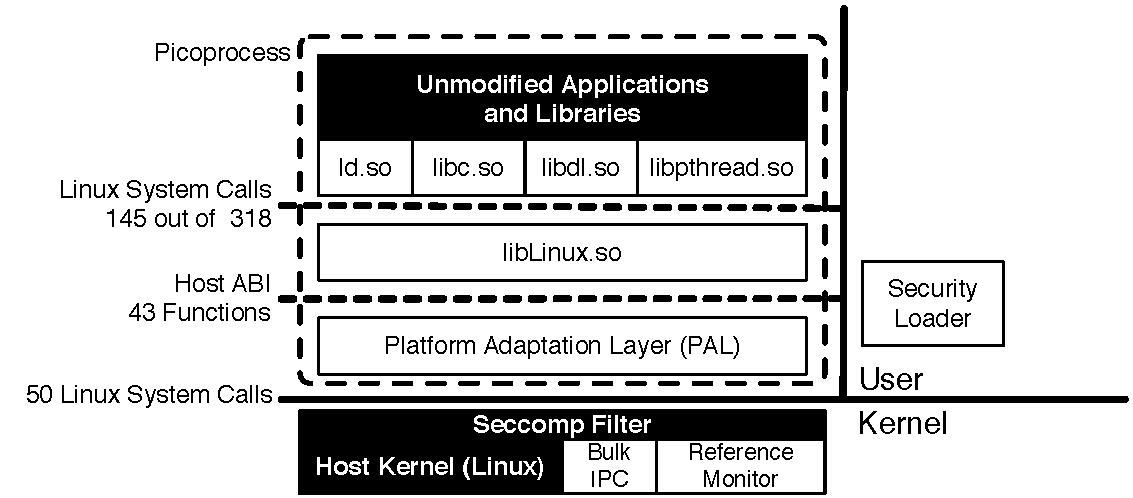
\includegraphics[width=32em]{arch.pdf}
\caption{Building blocks of \graphene{}.  Black components are unmodified.
We modify the four lowest application libraries on Linux:
{\tt ld.so} (the ELF linker and loader),
{\tt libdl.so} (the dynamic library linker),
{\tt libc.so} (standard library C),
and {\tt libpthread.so} (standard threading library), that issue Linux system calls as function calls directly to {\tt libLinux.so}.
Graphene implements the Linux system calls using a variant of the Drawbridge ABI, which is provided by the platform adaption layer (PAL).
A trusted reference monitor that ensures \libos{} isolation is implemented as a kernel module. Another small module is added for fast bulk IPC, but it is optional for hosts other than Linux.}
\label{fig:overview:arch}
\end{figure}


%\graphene{} shows the sufficiency of \thehostabi{} to support a rich Linux \libos{}.
As an example of this layering, consider the heap memory management abstraction. Linux provides applications with a data segment---a legacy abstraction dating back to original UNIX and the era of segmented memory. The primary thread's stack is at one end of the data segment, and the heap is at another.  The heap grows up (extended by \syscall{brk}) while the stack grows down until they meet in the middle.
In contrast, the host ABI provides only minimal abstractions for allocating, deallocating, and protecting regions of virtual memory.
This clean division of labor encapsulates idiosyncratic abstractions
in the library OS.


%These interfaces are host-independent \daniela{OS or kernel-independent}, as they tend to be very generic and easily
%implemented on any host OS kernel or VMM \daniela{postpone VMM for later}.

At a high level, a \libos{}
scoops the layer just below the system call table out of the OS kernel
and refactors the code as an application library.  
The driving insight is that there is a natural, functionally-narrow division point 
one layer below the system call table
in most OS kernels.
Unlike many OS interfaces, \thehostabi{} minimizes the amount of application state in the kernel, facilitating
migration. A \libos{} instance can programmatically read and modify its OS state, copy the state to another instance, and the remote instance can 
load a copy of this state into the OS---analogous to hardware registers.
A \picoproc{} may not modify another \picoprocs{}' OS states.



\papersubsection{Multi-process abstractions}
\label{sec:overview:libos:multiproc}


\issuedone{1.3.b}{An overview of multi-process support}
A key design feature of UNIX is that users compose simple utilities to create more significant applications.  Thus, it is unsurprising that many popular applications are multi-process---an essential feature missing from previous \liboses{}.
%This gap is filled by the \graphene{} \libos{}, which
%extends recent \liboses{} to support multi-process applications.
The underlying design challenge is minimally expanding a tightly-drawn isolation boundary without also exposing idiosyncratic kernel abstractions or re-duplicating mechanisms in both the host kernel and the library OS.

%requires a careful balance among the competing goals of 
%efficiency, host independence, and security isolation.
%The challenge, then, is minimal expansion of

%\vspace{5pt}
%\noindent {\bf Motivating Example.~}
For example, consider the process identifier (PID) namespace. In current, single-process library OSes, \syscall{getpid} could just return a fixed value to each application.
This single-process design is isolated, but the library OS cannot run a shell script, which requires forking and executing multiple binaries, signaling, waiting, and other PID-based abstractions.

%\paragraph{Design options.}
%Multi-process support requires extensions to the host ABI of recent, single-process library OS designs. Because multi-process abstractions, such as signals or System V IPC, tend to be idiosyncratic, an essential problem is identifying a minimal, host-independent substrate upon which  to implement OS-specific abstractions.
There are two primary design options for multi-process abstractions in \liboses{}: (1) implement processes and scheduling in 
the library OS; (2) treat each library OS instance as a process and distribute the shared POSIX implementation across a collection of library OSes.
\graphene{} follows the second option, which imposes fewer host assumptions.
%, maximize flexibility in mapping processes to physical resources, and facilitate inter-process security policy enforcement. % as enforcing security policies on related processes.

Multi-process abstractions
inside the library OS also possibly benefit from
hardware MMU virtualization, similar to
the model explored by Dune~\cite{belay12dune}.
However, this design reintroduces a duplicate scheduler and memory management.
Moreover, Intel and AMD have similar, but mutually incompatible MMU virtualization support,
which would complicate live migration across platforms.
None of these problems are insurmountable, and it would be interesting in future
work to compare both options.


In \graphene{}, multiple \liboses{} in multiple picoprocesses collaborate to implement shared abstractions. \graphene{} supports a rich of Linux multi-process abstractions including copy-on-write forking, \syscall{execve}, signals, exit notification, and System V IPC semaphores and message queues.
For instance, when process A signals process B on \graphene{}, A's library OS instance issues a query to B's instance over a pipe-like
RPC stream, and B's instance then calls the appropriate signal handler.
The host OS is unaware of the implementation
of multi-process abstractions,
as well as security isolation of the corresponding states.

%%% All collaborating \libos{} instances exchange messages as needed 
%%% to provide the application with a consistent view of 
%%% shared abstractions,
%%% such as


%\graphene{} approaches multi-processing by selectively replicating state and issuing remote procedure calls (RPCs) 
%%across multiple, collaborating
%library OS instances.
%Guests may work together to provide the unmodified multi-process application with
%coordination abstractions 

%%Shared abstractions on \graphene{}'s are implemented outside of the host, ensuring  host OS independence.
%% by implementing these
%%shared abstractions entirely
%%outside of the host kernel.
%%Shared abstractions are implemented outside of the host.
%%From the host kernel's perspective, 
%\graphene{} implements all shared abstractions by cooperatively managing the abstraction states over RPC streams.
%Single-process applications still service system calls from local state, and \graphene{}, includes optimizations to place state where it is most likely to be used, minimizing RPC overheads.
%The host reference monitor can easily isolate picoprocesses by 
%% \graphene{} design isolates \liboses{} by 
%%requiring all coordination to use 
%%explicit bytes streams \daniela{, pipe-like abstractions provided by the kernel. (suggestion: Reviewer  3)}.
%%Security isolation is enforced
%%by a kernel-level {\em reference monitor}, which can 
%%disconnect or prevent creation of a
%blocking all RPC messages, % between \liboses{} that should be isolated,
%without the need to understand the library OS details or semantics of these abstractions.
%In the PID example, only mutually-trusting picoprocesses can signal each other.
%%if the reference monitor prevents creation of RPC streams
%%across mutually untrusting \picoprocs{},
%%the \liboses{} cannot exchange signals.

%%% \graphene{} is designed to 
%%% The \graphene{} design leverages a number of optimizations to service application system calls 
%%% from local state whenever possible, and to minimize message passing overheads otherwise
%%%  (\S\ref{sec:namespaces:insights}).
%%% Our experience is that starting with a local system call design and then extending it to share state is relatively straightforward,
%%% and introduces little-to-no overhead when the request can be serviced locally.


The \graphene{} library OS is also capable of gracefully handling disconnection from other library OSes, facilitating dynamic application sandboxing.
RPC streams may disconnect at any time by either the reference monitor or at the request of a library OS.
%Message streams may be severed externally, by the reference monitor, or 
%one guest may simply disconnect from others to isolate itself.
%An application may disconnect itself from the 
%Any \graphene{} application may dynamically detach from the confederation, 
%or a host-level sandbox may dynamically separate two guests by severing their communication channels.
When a picoprocess is disconnected, the library OS will handle the subsequent
divergence, %and the library OS will will fork these abstractions
{\em transparently} to the application.
For instance, if a child process disconnect RPC streams from the parent by the reference monitor, the library OS will interpret the event as if the other process terminated, close any open pipes, and deliver exit notifications.
% \daniela{(applications run unmodified) - Reviewer 1 asked clarification on transparently}.

%% A key insight behind our design is that the common use case for these \daniela{cooperating} abstractions
%% is between a pair of processes.  Thus \graphene{} leverages a number of optimizations 
%% to reduce broadcast messages, avoid replication of needless state,
%% and service requests locally


\paragraph{Comparison with microkernels.}
The building blocks of \graphene{} are very similar to the system abstractions of a 
microkernel~\cite{liedtke95sosp,klein09sel4,elphinstone13microkernels,liedtke93sosp,chen93memory,baron1985mach-1,accetta86mach}, except a microkernel often has an even narrower, more restricted interface than the host ABI.
%such as the port and
%message abstractions of Mach~\cite{
A multi-server microkernel system, such as GNU Hurd~\cite{hurd} or Mach-US~\cite{stevenson95mach-us}, implements Unix abstractions across a set of daemons that are shared by all processes in the system. \graphene{}, on the other hand, implements system abstractions as a library in the application's address space and coordinates library state among \picoprocs{} to implement shared abstractions. \graphene{} guarantees isolation equivalent to running 
an application on a dedicated VM; it is similar to implementing the security isolation model on a multi-server microkernel by running a dedicated set of service daemons for each application.

%%% \graphene{}'s differences are motivated by two considerations: efficient support of both stand-alone, 
%%% single-process applications and multi-process applications; as well as flexible security isolation. 
%%% \graphene{} contributes techniques to seamlessly and efficiently transition 
%%% between single-process and multi-process support, as well as adapting 
%%% some known techniques to a new environment.

%The \graphene{} host ABI could be described as a hybrid microkernel, which also exposes the file system and network of the host kernel.
%Similarly, picoprocesses are assumed to be provided by a production OS, like Linux or \win{}, or by a Type 2 hypervisor.  A bare metal hypervisor could potentially export a PAL, but would require services from a trusted VM, such as Xen's dom0~\cite{barham03xen}.
%%or the \pal{} would implement more thread scheduling, networking, and file system code;
%%or the \pal{} ABI would change to push this code into the \libos{}.
%Arguably, recent library OS designs might be improved by rethinking the division of labor, but this is beyond the scope of this thesis.

%\paragraph{Alternatives.}
%Another approach to support multi-process applications in a library OS would be to use hardware MMU virtualization such as nested paging used by a system like Dune~\cite{belay12dune}
%in order to implement a second process abstraction, memory manager, and scheduler in the library OS.
%This approach threatens the efficiency benefits of deduplicating these features.
%A final option is exposing additional system interfaces, such as signals, by adding more system calls to a picoprocess. This approach undermines compatibility, as many of these coordination abstractions tend to be very OS-specific.
%%Unix signals vs.\ \win{} events, {\tt waitpid()} vs.\ blocking on a process handle, etc.
%%Although legacy OSes do enforce some access control rules on coordination abstractions,
%%kernel developers must audit and add hooks to millions of lines of code.
%%As a result,
%%users have lost confidence that a traditional OS can comprehensively enforce 
%%security isolation on these abstractions---a key motivation for using VMs
%%for security isolation.


%Systems must strike a careful balance between the competing goals of
%security isolation and multi-process coordination.
%Multi-process applications require OS-managed coordination abstractions such as signals, process exit notification, and System V IPC.
%These coordination abstractions operate within shared namespaces, such as the process ID namespace and the System V key space.
%These coordination APIs and namespaces must be consistent among coordinating processes, but can undermine security isolation among unrelated processes on the same host.
%System designs generally only meet one goal: traditional OSes have a rich but porous coordination interface, while sandboxing systems and VMs are strictly isolated.
%This thesis demonstrates that this unfortunate trade-off is not fundamental.
%coordination or isolation.  


%Traditional OS kernels typically provide  rich multi-process coordination APIs, but this richness also makes for a very porous attack surface area.  For instance, on \win{}, a program may inject libraries and create threads in another program~\cite{windows-dll-inject}; 
%similarly, unchecked file descriptor inheritance in Linux can lead to security problems~\cite{close-on-exec}.  
%Although legacy OSes do enforce some access control rules on these abstractions, kernel developers must audit and add hooks to so much code that users have lost confidence that an OS can comprehensively enforce security isolation on these abstractions.

%For achieving strong security isolation on applications, users have turned to VMs.
%For instance, if two customers host their websites in the same cloud service, the customers will insist on running their web servers in separate VMs for security.
%VMs take a heavy-handed approach to security isolation---ensuring that every application has a dedicated OS kernel in a hardware-isolated address space.
%Although virtual machines isolate applications and provide legacy OS abstractions within a VM, coordinating applications must be statically placed in the same VM,
%and cannot dynamically move to a separate VM.
%For instance, consider a web service running inside of a VM that wishes to isolate requests for different users in different VMs after authentication.  The web server administrator must statically create a VM for each user, introducing substantial
%overhead; and the developer loses convenient IPC abstractions and must rewrite large swaths of code.

\section{Summary}
\label{sec:graphene:summary}

The \graphene{} design is centered around
building a para-virtualized layer, which can reuse the OS components for reproducing Linux system interfaces.
%instead of building arbitrary compatibility layers for reproducing the system interface.
%constantly porting the significant  of the existing system interface.
%In \graphene{}, 
\graphene{} defines a host ABI, as a new boundary between the OS and user space.
The host ABI is simple enough to port (containing \palcalls{} functions),
and exports sufficient functionality for virtualizing a primary part of the system API components.
A library OS is built upon the host ABI,
and implements \graphenesyscalls{} Linux system calls to reuse unmodified Linux applications.
\graphene{} decouples the development for a compatibility layer,
from host-specific challenges to building OS features, and isolating applications from other malicious tenants.



%\sysname{} extends library OS designs 
%to include multi-process APIs required by common applications, such as a shell or 
%web server.
%\sysname{} demonstrates efficient, selective
%coordination of shared state across multiple library OS 
%instances---maintaining host independence.
%%simplifying security sandboxing of otherwise unwieldy OS features.
%Applications on \sysname{} enjoy both 
%strong security isolation with acceptable performance and low memory overheads.
%% from unrelated programs 
%%and seamless shared namespaces 
%%among a group of coordinating guests.
%%% Although this paper focuses on distributed coordination
%%% to facilitate the efficiency benefits,
%%% expect our experiences with distributed coordination 
%%% may also be particularly relevant to highly scalable OS designs, 
%%% which avoid the bottlenecks of shared OS data structures~\cite{baumann09barrelfish, song11eurosys}.
%%Graphene's overheads are acceptable and the memory 
%%footprint is substantially lower than a VM.



%% , which could benefit from the reduced memory footprint
%% in a cloud 

%% by introducing a novel design for  coordination APIs. 
%% to a new OS (Linux),
%% new classes of applications,
%% and introduces a
%% %an alternative design point for storage virtualization.
%% Our results further demonstrate the feasibility of the library OS model.
%% % generally,
%% Applications on Graphene enjoy both 
%% strong security isolation from unrelated programs 
%% and seamless shared namespaces 
%% among a group of coordinating guests.
%% Although we explore this concept in a library OS,
%% we expect the namespace coordination framework 
%% could also be adapted to limit the attack surface area between
%% processes in a traditional OS.
%% We expect these experiences with distributed coordination 
%% may also be particularly relevant to highly scalable OS designs, 
%% which avoid the bottlenecks of shared OS data structures~\cite{baumann09barrelfish}.
%and specifically of content-addressable storage as the primary virtual storage abstraction.
%%% This work opens up a number of interesting questions for future work, 
%%% including studying opportunities for low-level storage optimization within the CAS server,
%%% making CAS the root file system,
%%% eliminating storage management in the host kernel, and 
%%% investigating the impact of frequent migration among devices.

\begin{comment}
Enabling legacy applications in a restricted environment,
such as \picoprocs{} or enclaves,
requires extra effort for mitigating the limitations of platforms,
in order to support typical OS personalities.
\graphene{}, as described in this chapter, extends the existing \libos{} designs
from isolating single-process or unshared abstractions
to include multi-process APIs required by many UNIX applications,
such as servers or shell scripts.
The challenge that \graphene{} primarily overcomes
is the requirement for coordinating shared states across multiple \picoprocs{},
to provides a collaborative, unified OS view.
Essentially, \graphene{} implements all shared, multi-process abstractions
and OS states
based on coordination over host-provided, pipe-like RPC streams.
The RPC-based, distributed OS implementation enables multi-process support in \graphene{}, with minimal extension to the host interface,
and a sweet-spot for enforcing inter-application security isolation,
by simply sandboxing the RPC streams.
Such a model largely reduces the complexity of
enforcing security isolation
on idiosyncratic multi-process abstractions
and shared states.
Because the corporative nature of \picoprocs{} in \graphene{},
an application can even dynamically impose sandboxing on one of its processes,
to reflect per-process, variable security policies.
\end{comment}

\begin{comment}
In principle, we attempt to use \graphene{} to justify the platform independence
of the \libos{} design,
without sacrificing its qualitative benefits,
such as isolating mutually-untrusting applications
and a narrow attack surface to kernels.
\graphene{} implements a considerable number of common Linux system calls,
to support popular, modern applications
such as Apache web server, GNU Make, OpenJDK \java{} VM and the Python runtime.
\graphene{} translates the high-level system APIs used by applications
to a host ABI
inherited and extended from a previous Windows-compatible \libos{}~\cite{porter11drawbridge}.
In addition, we port the \pal{} (Platform Adaption Layer) of \graphene{}
to various platforms,
including FreeBSD, OSX, Windows, and even a more restricted environment, the \intel{} \sgx{} enclaves.
In particular, \graphene{} being ported to \intel{} \sgx{}
(\graphenesgx{})
can isolate applications --- either single-process or multi-process
--- on a host where neither the operating system nor the hardware (except the CPU package)
is trusted by the applications. 
Overall, \graphene{} shows that,
by simply porting the reasonably sized host ABI
to a new platform,
a whole large spectrum of legacy applications tested on the previous platforms
can be activated all together.
\end{comment}

\makeatletter
\def\input@path{{}}
\makeatother
\graphicspath{{}}
\subsection{Shielding Multi-Process Abstractions}
\label{sec:multiproc}

Many Linux applications use multi-process abstractions,
which are implemented using copy-on-write fork and in-kernel
IPC abstractions.
In SGX, the host OS is untrusted, and enclaves cannot share protected memory.
Fortunately, \graphene{} implements multi-process support
including {\tt fork}, {\tt execve}, signals, and a subset of System V IPC,
using message passing instead of shared memory.
%The {\it zero-sharing} nature of \graphene{} makes it possible
Thus, \graphenesgx{} implements multi-process abstractions in enclaves
without major library OS changes.
This subsection explains how
%we will describe how \graphenesgx{} securely creates
\graphenesgx{} protects
 multi-processing abstractions from an untrusted OS.


%% \fixme{need to polish this subsection}

%% Upon existing platforms using \sgx{}, there is no
%% multi-process abstractions of any kinds that has been supported so far,
%% either in \haven{} or other systems.
%% The main challenge against
%% implementing multi-process abstractions in enclaves
%% is to share enclave pages,
%% for either Linux-style copy-on-write {\tt fork}'ing or
%% sharing abstraction states.
%% Fortunately,


%processes in new enclaves,
%%for supporting
%        {\tt fork}, {\tt execve},
%and inter-process communication
%(namespace coordination, signals, System V IPC, etc)
%with process isolation.

%\subsubsection{Forking into new enclaves}
%\label{sec:multiproc:fork}

\begin{figure}[t!]
\centering
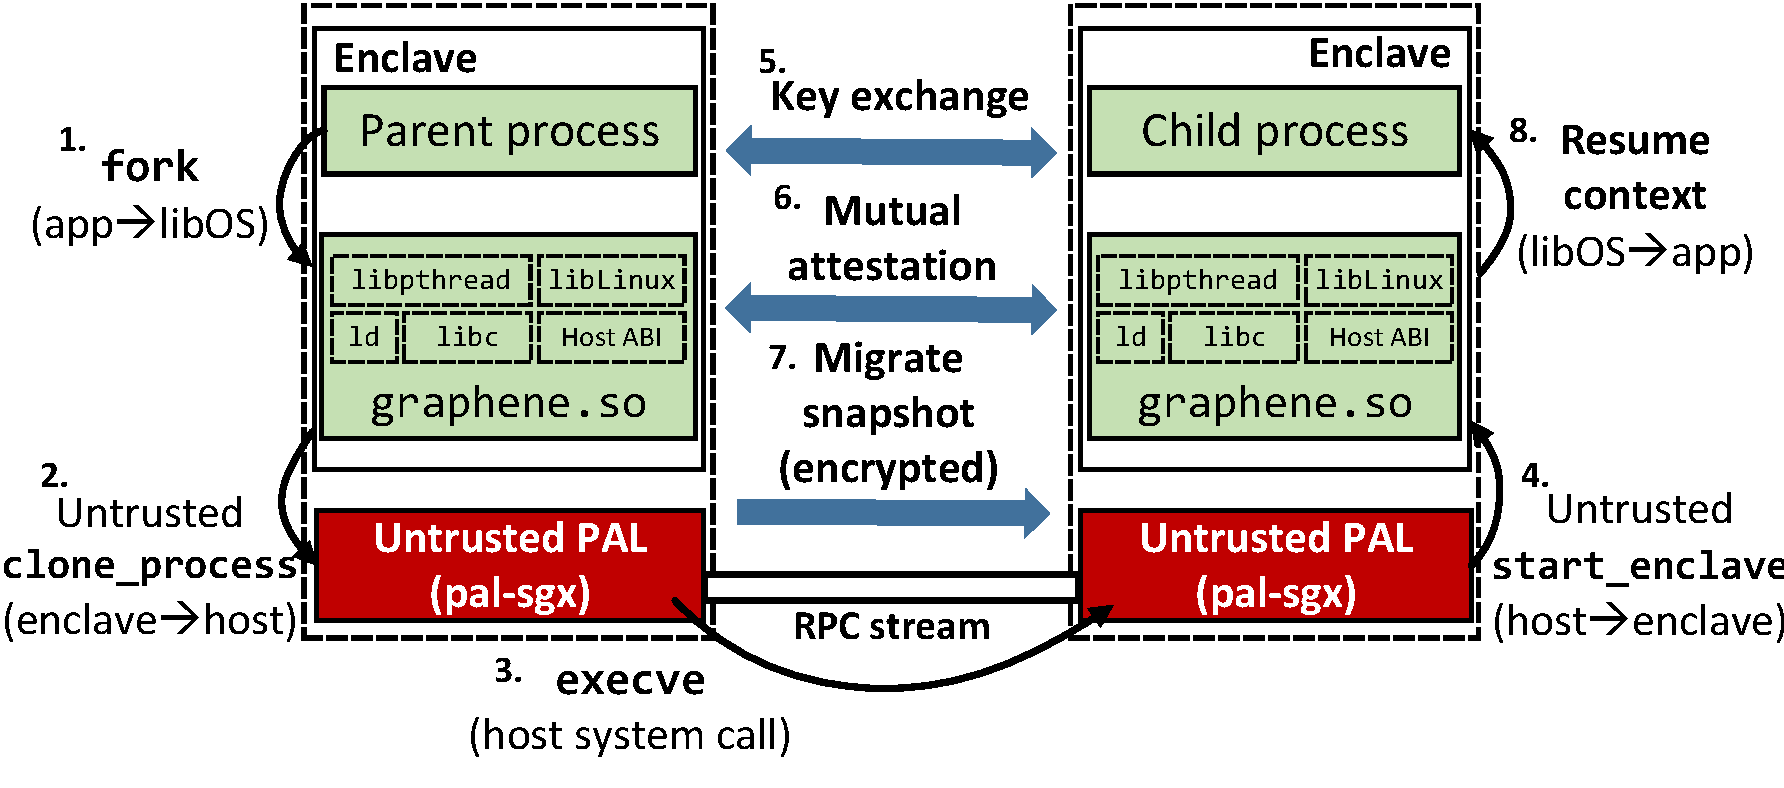
\includegraphics[width=\linewidth]{fork.pdf}
\caption{Process creation in \graphenesgx{}.
Numbers show the order of operations.
When a process forks, \graphenesgx{} creates a new, clean enclave
%calls {\tt execve} system call
on the untrusted host.
%to create a clean enclave with the same \libos{} image.
Then the two enclaves %build up the mutual trust by
exchange an encryption key, validates the CPU-generated attestation of each other,
and migrates the parent process snapshot.}
\label{fig:fork}
\end{figure}

\begin{comment}
To secure process creation across enclaves,
\graphenesgx{} is capable of building up the trust to newly launched enclaves,
through cooperation with an untrusted host.
Once a clean and trusted new enclave is launched,
The parent process will send a snapshot to the new one,
to create a clone of itself.
Snapshotting and migrating process states
is a feature robustly implemented and heavily used in \graphene{} \libos{},
of which we simply inherit the design.
\end{comment}

Process creation in \graphenesgx{} is illustrated in Figure~\ref{fig:fork}.
When a process in \graphenesgx{} forks into a new enclave,
the parent and child will be running the same manifest and binaries,
and will have the same measurements.
%\fixme{rewrite this part. check this. dp: check my rewrite}
Similar to the process creation in Graphene, the parent and child enclaves are connected with a pipe-like RPC stream, through the untrusted PAL.
As part of initialization, the parent and child will exchange a session key over the unsecured RPC stream, using Diffie-Hellman.
The parent and child use the CPU to generate attestation reports, 
which include a 
512-bit field in the report to store 
a hash of the session key
and a unique enclave ID.
The parent and child exchange these reports to authenticate each other.
Unlike remote attestation, local attestation does not require 
use of Intel's authentication service (IAS).
% then exchange attestation reports \fixmedp{right?} generated by the CPU (unlike remote attestation, local attestation does not require Intel-owned services to verify the CPU).
% which will prove that the attested enclave is the one and only one that agrees on the key.
% sensitive data from being divulged to an attacker during \syscall{fork}.
%For example, to prevent a man-in-the-middle attack, between the parent and child,
%we use
%a 512-bit field
%in the CPU-signed attestation to store a hash of the session key
%and a unique enclave ID, which will prove that the attested enclave is the one and only one that agrees on the key.
%generated and signed by \sgx{}.
%Once the child enclave is launched, as part of initialization,
%the parent and child will exchange attestation generated by the CPU,
%exchange a signed session key using Diffie-Hellman, and then 
%establish a TLS connection over an inter-enclave RPC stream.
% after creating a signed session key using a key exchange algorithm like Diffie-Hellman.
%then use a session key to generate an encrypted connection.
%\fixmedp{I still don't understand the following text; let's discuss}
%What the Intel CPU provides here is the confidential CPU secret that the inter-enclave attestation is based on. The attestation establishes a trusted path within enclave groups to exchange library OS state.
%\fixmedp{IF time, clarify what HW provides here or how it works}
Once the parent and child have authenticated each other, the parent establishes a TLS connection over the RPC stream using the session key.
The parent can then send a snapshot of itself over
the TLS-secured RPC stream, and the snapshot is resumed in the child process, making it a clone of its parent.
This mutual attestation and encryption strategy
% between the parent and child
prevents a man-in-the-middle attack between the parent and child.
%To build up the trust, the two processes will open an encrypted channel
%using a session key,
%and exchange attestation generated by the processor.
%Once both sides have confirmed the integrity of the other,
%the parent process is safe to send its snapshot, encrypted, to the child
%through the said channel.
%The child process will resume the snapshot in its own enclave,
%making it a clone of its parent.


%The fork design in \graphenesgx{} provides several security measures.
%First, mutual attestation and encryption between the parent and child
%prevent sensitive data from being divulged to an attacker during {\tt fork()}.
%To prevent a man-in-the-middle attack, between parent and child,
%we use
%a 512-bit field
%in the attestation structure generated and signed by \sgx{}.
%We use this field to store a SHA-256 hash of the session key,
%and a unique enclave ID,
%\fixmedp{also a piece of intuition missing here; let's discuss}
%to prove that the attested enclave is the one and only one that agrees on the key.

%% Forking in \graphenesgx{} mainly defends against 3 types of attacks
%% from the untrusted host:

%% \begin{compactenum}

%% \item The host pretends to be the child enclave, to expose the process snapshot
%% sent from the parent.

%% \item The host pretends to be the parent enclave, to compromise the
%% child process using a malicious process snapshot.

%% \item The untrusted host becomes a man-in-the-middle, which bounces
%% encrypted messages between the child and parent enclaves, with session keys
%% negotiated with both sides.

%% \end{compactenum}

%% As described earlier, attacks 1 and 2 are prevented by mutual attestation
%% between the parent and the child,
%% and encrypting the channel for sending the snapshot.
%% The attestation signed by the processor proves that both entities communicating
%% are valid \graphenesgx{} enclaves,
%% and encrypting the channel prevents the snapshot being eavesdropped or
%% counterfeited by the host.

%% To defend against attack 3 (the man-in-the-middle attack), we take advantage of
%% a user-customized 512-bit field
%% in the attestation structure generated and signed by \sgx{}.
%% This field is filled with a SHA-256 hash value of the agreed session key,
%% and the current enclave ID,
%% to prove that the attested enclave is the one who agrees on the key.

Once a parent enclave forks a child, by default, the child is fully trusted.
To create a less trusted child, the parent would need to sanitize its snapshot,
similar in spirit to the close-on-exec flag for file handles.
%to maintain its own security,
%because the migrated snapshot discloses all information in the parent.
%Unless the binary run in the parent enclave ensures
%that no secrets is stored in the enclave memory at the time of snapshotting,
%the parent enclave cannot simply drop the trust against the child.
For example, a pre-forked Apache web server may want to keep worker
processes isolated from the master %\fixmedp{Right nomenclature}, %that responds to HTTP requests isolated,
to limit a potential compromise of a worker process. %avoid being compromised by one attacked worker.
\graphenesgx{} inherits a limited API from \graphene{}, 
for applications to 
isolate themselves from untrusted child processes,
%\graphenesgx{} inherits this dynamic process isolation feature.
but developers are responsible for purging confidential information
before isolation.

\paragraph{Supporting \syscall{execve}.}

Unlike \syscall{fork}, \syscall{execve} 
starts a process with a specific executable, often different from the caller.
When a thread calls \syscall{execve} in \graphenesgx{},
the \libos{} migrates the thread to a new process,
with file handles being inherited.
%with clean process states except opened files cloned from the parent.
Although the child does not inherit a snapshot from its parent,
it can still compromise the parent 
by exploiting potential vulnerabilities in handling RPC, 
which are not internally shielded.
In other words, \graphenesgx{} is not designed to share library OS-internal
with untrusted children.
Thus, \graphenesgx{} restricts \syscall{execve} to only launch trusted executables, which are
specified in the manifest.


%  main challenge to supporting \exec{} is to
%ensure only trusted binaries can be created as child processes.
%loaded into new enclaves as child processes.
%The trust between parent and child must be mutual,
%or applications won't be secure.
%unless the two enclaves are strictly isolated.
%To secure \exec{},
%\graphenesgx{} stores the enclave measurements of executable binaries that can be trusted as children processes
%inside the manifest file.
%To identify binaries that can be trusted (either as parents or children)
%during process creation,
%\graphenesgx{} requires each binary ported for an application,
%to be shipped with a list of binaries that can be \exec{}'d,
%and those that can be callers of \exec{} to the said binary.
%Each binary in the list is identified by its measurement, which is mutually attested
%between the parent and the child during process creation.
%This list must be signed by a private key provided by the client,
%while the public key must be included in the enclave measurement of the binary.


\paragraph{Inter-process communication.}
\label{sec:multiproc:ipc}

After process creation, parent and child processes will cooperate
through shared abstractions,
such as signals or System V message queues, via RPC messages.
While messages are being exchanged between enclaves,
they are encrypted, ensuring that these abstraction are protected
from the OS.

%For \libos{}, OS states for these shared abstractions must be shared
%though inter-process coordination, for mainly two purposes.
%First, for each abstraction, \libos{} needs to maintain the state
%in one of its instances.
%Second, \libos{} must maintain the namespace states to identify and locate the
%abstraction states.
%\graphene{} implements a wide range of multi-process abstractions and namespaces,
%by coordinating OS state over RPC streams, rather than using shared memory. 

%% dp: this point already made above
%Because SGX does not allow enclaves to share trusted memory,
%the fact that the original Graphene design did not require shared memory
%made porting to SGX considerably easier.

% (pipes).
%Such a design is perfect for porting multi-process applications to enclaves.

%Thus, by coordinating OS state via 
%Thus, the benefit of coordinating OS state via message passing 
%is that 
%the enclaves need no will not share any memory to
%coordinate abstraction states,
%simplifying the support and security of library OS.
%and the RPC streams can be secured by the enclaves instead of the host.
%By encrypting the RPC streams among related processes,
%inter-process communication is easily protected from the untrusted OSes.
%In \graphene{}, security isolation among multi-process abstractions,
%regardless of their semantics,
%are enforced by isolating the RPC streams used for coordination.
%Unfortunately, \graphenesgx{} cannot trust the host to faithfully isolate
%the RPC streams.
%Each enclave launched for an application must secure inter-process coordination
%spontaneously, by only communicating to enclaves that it has attested
%and exchanged secret keys with.
%Because inter-process coordination is completely transparent
%to the applications,
%all information sent over RPC streams must be encrypted,
%because \libos{} cannot determine whether the information may contain any secret.






\section{Implementing the Host ABI}
\label{sec:linux:impl}


The majority of \pal{} calls are simple wrappers for similar Linux system calls, 
adding less than 100 LoC on average for translation between \pal{} and Linux abstractions.
The largest \pal{} calls are for exception handling, synchronization, and picoprocess
creation, which require multiple system calls and range from 500--800 LoC each.
Creating a new picoprocesses internally requires a {\tt vfork} and {\tt exec} of a clean 
application instance, and would be more efficiently implemented in the kernel.
Finally, the other major \pal{} components are an ELF loader (2 kLoC), headers (800 LoC),
and internal support code (2.3 kLoC).

%\paragraph{Alternative \pal{} Ports.}
%We prove the platform independence of \graphene{}
%by porting \pal{} to \emph{FreeBSD}, \emph{OSX} and \emph{Windows}.
%With the alternative host \pal{}, unmodified Linux binaries,
%along with {\tt glibc} and {libLinux},
%can be transparently run on the host.
%For FreeBSD,
%only 1.2 kLoC of the host \pal{} code need to be rewritten,
%which are significantly less than FreeBSD Linux compatibility module (10.8 kLoC).
%\pal{} components including ELF loader and internal support code can be shared by any \pal{} ports.

%\fix{We leave host \pal{} ports to non-unix OSes like Windows as future work,
%but previous works~\cite{porter11drawbridge,baumann13bascule} have already shown it feasible.}

\begin{table}[t!b!]
\footnotesize
\centering
\begin{tabular}{|l|rr|}
\hline
{\bf Component} & {\bf Lines} & ({\bf \% Changed})\\
\hline
GNU Library C ({\tt libc}, {\tt ld}, {\tt libdl}, {\tt libpthread}) & \libclines{} & $0.07\%$ \\
\hline
Linux Library OS ({\tt libLinux}) & 31,112 & \\
Linux host \pal{} & 11,644 & \\
Extra code for Linux \sgx{} host \pal{} & 9.354 & \\
% updated by Chia-Che on Oct. 10, 2013
\hline
%Storage Server & \fixmedp{XX} & \\
Reference monitor bootstrapper & \reflines{} & \\
Linux kernel reference monitor module ({\tt /dev/graphene}) & \sandboxmodlines{} & \\
Linux kernel IPC module ({\tt /dev/gipc}) & \gipclines{} & \\
\hline
\end{tabular}
\caption[Lines of code written or changed in \graphene{}]
{Lines of code written or changed to produce \graphene{}.  Applications and other libraries are unchanged.}
\label{tab:graphene:loc}
\end{table}


%% * most calls are a wrapper, \fixmedp{XX} LoC on average.
%% * Exception handling, sync, and process creation were harder (500-800 LoC each).  Process creation requires a clean instance (vfork+exec), would be simpler to implement in kernel.
%% * Other major components: ELF loader (2kLoC), headers(800 LoC), internal support code (2300 LoC)


%\fixmedp{Chia-Che, update LoC table}



\paragraph{Synchronization.} Perhaps surprisingly, implementing Linux
synchronization appears substantially easier than Windows synchronization, 
as {\tt libLinux} did not require all of the various
synchronization ABIs provided by Drawbridge.
We believe the reason for this is that Linux has consolidated 
all user-level synchronization primitives to use futexes~\cite{franke02futex},
which are essentially kernel-level wait queues.
%In Windows parlance, this is simply an Event associated with a virtual address.
%Thus, our effort implementing synchronization was relatively straightforward.

%\papersection{\Thehostabi{}}
\label{sec:overview:host}

\issuedone{1.1.b}{Describe \thehostabi{} specification}
The development of \graphene{} starts with defining a simple host ABI (application binary interface) called \thehostabi{},
containing only OS abstractions essential to target applications.
%and is easily ported to different platforms.
%and minimal specifications for the host OSes and hardware.
%The host ABI is a new boundary between OSes (or hypervisors) and applications.
\Thehostabi{} separates
the implementation of an existing system API (application programming interfaces), which determines the compatibility against applications,
from hardware abstraction features, such as file systems, network stacks, and device drivers. 
\graphene{} moves the system API components
to a \libos{} in the userspace and reimplements the functionality using \thehostabi{}.
To port \graphene{} to a new host OS or hardware,
OS developers only have to implement \thehostabi{} on the target host system API,
%to new host OSes and hardware,
instead of paying a tremendous cost to translate the whole system API specification. Figure~\ref{fig:overview:porting} illustrates the porting process of \graphene{}.



%The host ABI separates the low-level, hardware management features, from the idiosyncrasy of system interface. 
%\graphene{} moves the upper layer of OS components,
%including the system calls and namespaces, into an library OS,
%leaving \thehostabi{} 
%as a narrowed interface to the host OSes and hardware.
%The host ABI intends to minimize the development effort on each host OS or hardware
%to mitigate the interface distinctions,
%to simply porting the OS abstractions defined in \thehostabi{}.


\begin{figure}[t!]
\centering
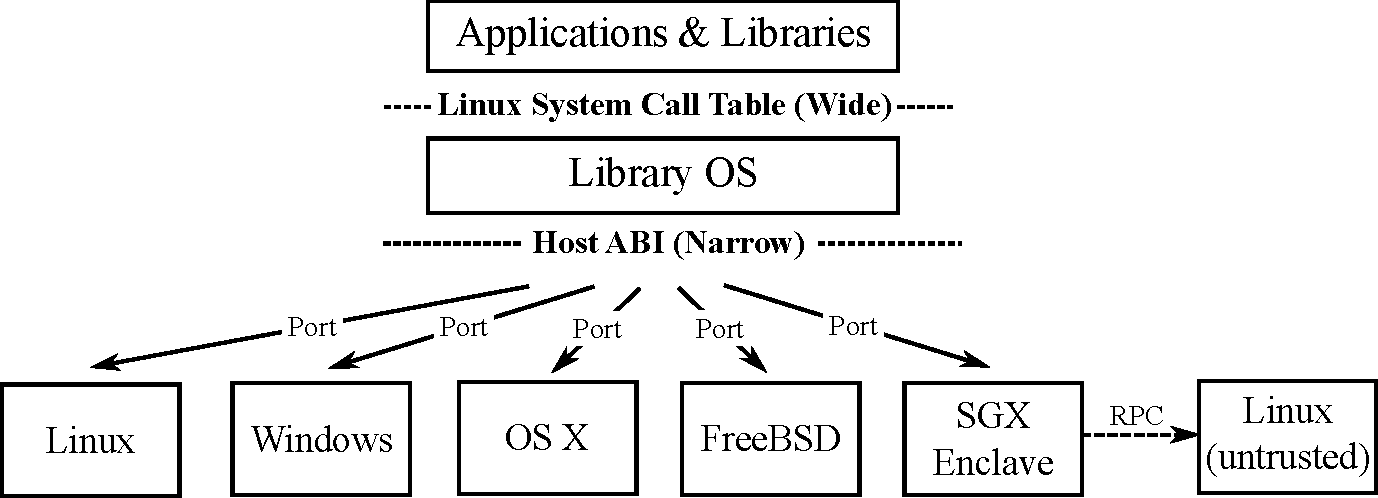
\includegraphics[width=30em]{porting.pdf}
\caption{Porting model of \graphene{}.}
%\vspace{-.1in}
\label{fig:overview:porting}
\end{figure}



\papersubsection{Platform Adaption Layers (PALs)}
\label{sec:overview:host:pal}


For each host OS or hardware, \graphene{} uses
a thin library called a {\bf platform translation layer (PAL)}
to translate among host interfaces.
%is loaded below the library OS, to translate each functions in \thehostabi{} to native system interfaces.
The main purpose of a PAL is to mitigate the semantic gap
between \thehostabi{} and
native host system APIs.
%The effort of PAL development is per host OS, whereas the library OS implementation is reusable on every hosts. %The simplicity of \thehostabi{} can be also estimated by the effort of implementing a PAL for each host.
By implementing a PAL on a new host OS or hardware,
users can reuse
the same \libos{} to run the same collection of unmodified Linux applications.
%To keep the porting effort low,
%the development of a PAL must be straightforward
%for average OS developers.
%to achieve with limited efforts.
%Based on the principle of porting simplicity, PAL development must be straightforward
%for average developers.







%The host ABI is defined for the simplicity of porting, as well as the sufficiency for implementing a library OS compatible to Linux.
%First of all, the number of host functions included in \thehostabi{}
%is much smaller than the number of system calls in a commodity OS such as Linux. 
\graphene{} currently contains PAL implementations for several popular OSes,
including Linux, \win{}, \osx{}, and FreeBSD.
%and \sgx{} with an untrusted Linux kernel.
Most of these OSes provide a POSIX-like system API similar to \thehostabi{}.
Due to the similarity, translating most of \thehostabi{} to one of the system APIs
are straightforward for average OS developers.
\Thehostabi{} is also much smaller than the actual POSIX API, making it extremely portable.



A part of \thehostabi{} may be challenging to port
on an OS,
due to unexpected system assumptions made by the OS.
For instance, \win{} does not support
fine-grained memory deallocation for de-privileged applications.
To implement system calls like \syscall{munmap} and \syscall{mprotect},
\graphene{} needs host ABIs to
deallocate or protect virtual memory pages at page granularity.
%A workaround is to change memory mappings at the physical page level,
%but will require running the \win{} PAL with root permissions.
%This type of porting challenges
%tends to be results of design decisions or assumptions made by OS developers.
%A \libos{} can potentially design
%different emulation strategies
%to compensate missing host abstractions.
A few host abstractions such as a bulk IPC feature are
optional to the host ABI;
if a host OS does not support these abstractions,
the \libos{} must fall back to alternatives. 

%In our experience, the development of a PAL is around ten thousand lines of code.

%For each port, the amount of code written for implementing \thehostabi{} is at the order of magnitude of thousands of lines of code, which is much more manageable than implementing a flat translation layer for system interfaces.


\begin{comment}
Based on the experience in \graphene{},
it is hard to ensure the portability of \thehostabi{} on every potential hosts.
%even a host ABI specialized for simplicity cannot guarantee to be portable on every hosts.
A host may simply lacks the functionality
for implementing a \hostapi{}.
The assumption is, maintaining the compatibility of \thehostabi{} poses a much less challenge than maintaining the whole system API.
Besides, the library OS may flexibly switch among emulation strategies
to compensate the absence of certain host abstraction.
As an example,
bulk IPC is optional in \thehostabi{} since its first definition,
due to the expectation
that implementing the feature may not be feasible on some hosts.
If bulk IPC is not available,
the library OS can fall back to RPC-based IPC, with a reasonable amount of performance penalty.
In the worst case, if there is no emulation strategies
to compensate for the absence of a \hostapi{},
user can predict the affected applications and avoid running these applications
on specific hosts. 
%at least users can predict whether an application will be affected and thus cannot run on certain hosts.
\end{comment}


%For a host OS that does not support ELF binaries, the PAL must follow the binary format which the host OS accepts, such as the Portable Executable (PE) format on \win{}.
%The PAL is the only layer in the user space which cannot be reused
%across different hosts. Besides the PAL, all of the other binaries in the user space are fully reusable, including the library OS, the supporting libraries, and the application executable.



%The host abstractions map to several common system calls in a commodity OS.
%For example, \funcname{StreamRead} and \funcname{StreamWrite} can directly map to the POSIX functions \funcname{pread} and \funcname{pwrite}, which are available in most OSes including Linux, BSD, \osx{}, and \win{}.
%More than half of the functions in \thehostabi{} can be counted toward this category.
%The rest of the host abstractions are either specific to Linux
%(e.g., TLS support),
%or belong to the POSIX functions that are not shared with commodity OSes
%(e.g., \funcname{mmap} on \win{}).
%The PAL emulates these host abstractions, using existing system interfaces available on the host OS, unless the software emulation is fundamentally impossible (e.g., restricted by the system interfaces), or too expensive (e.g., high overhead from copying data).



\papersubsection{Definitions and design principles}
 

\graphene{} defines \palcallnum{} calls in \thehostabi{} (also called \hostapis{}),
with a set of host abstractions
sufficient for \libos{} development.
%The host ABI defines the interaction between the library OS and a specific host.
%The \graphene{} library OS can be deployed on any ``host'' where \thehostabi{} has been ported.
This thesis defines
a {\bf host} of \thehostabi{}
to be an OS or hypervisor
which contains enough OS functionality for running a standalone application or virtual machine.
Most of the host targets in \graphene{}
are monolithic OSes,
including Linux, \win{}, \osx{}, and FreeBSD.
%which has defined a massive system API for programmability.
A monolithic OS 
usually contains a massive amount of system APIs,
which is sufficient for
implementing \thehostabi{}.


A special example of a host
is an \sgx{} (Software Guard Extensions) enclaves~\cite{intelsgx},
which
restricts OS functionality for security reasons.
The restrictions on \sgx{}
are results of a strong threat model
which distrusts any OS features except ones that are virtualized by the CPUs or migrated into enclaves.
The only way to obtain any missing OS features such as storage or networking
is to request through RPC (remote procedure call).
Requesting untrusted OS services through RPC also introduces new security threats that application developers tend not to anticipate~\cite{checkoway13iago,osdi16scone}.
Due to all the compatibility and security challenges discussed above,
this thesis uses \sgx{} as a representative example of a host
with unusual assumptions (e.g., threat models) and restrictions
compared to a monolithic OS.

%An innovative hardware abstraction like \sgx{} (software guard extensions)
%imposes unique assumptions and restrictions
%on a commodity OS,
%%creates a special host on top of Linux or \win{},
%%with unique interfaces and specifications regarding the host OSes.
%and thus creates a special host above the OS.

%If an OS has mutated or tweaked the interface for a hardware platform,
%such as an \sgx{} enclave 
%running on an untrusted Linux kernel,
%the combination of the OS (Linux) and the hardware platform (\sgx{}) is considered a specialized host.
%Especially, the \sgx{} port of \thehostabi{} faces several unique challenges,
%which will be discussed in Chapter~\ref{chap:sgx}.


\begin{comment}
%\fixme{each sentense should be a paragraph; starting the 2nd sentence}
\fixmedp{start with a strong opening stating the rationale}
The host ABI of \graphene{}
define functions needed from a host, in order to implement the library OS for reusing applications.
%to reuse an application and all its supporting libraries, including the \graphene{} library OS.
Each host of \graphene{} contains an OS and a hardware platform, either of which causes compatibility issues for running unmodified applications.
OS developers can port the library OS to a new host,
by simply reimplementing the narrowed host ABIs using abstractions available on the host.
%a new host platform.
%For each host which requires the compatibility for unmodified Linux applications, one only has to implement the narrowed host ABIs,
%instead of reimplementing the bloated, ``legacy'' system interfaces
%needed by the applications.
By implementing \thehostabi{}, OS developers skip the painful process of rebuilding the whole system interfaces of a commercial OS such as Linux.
The host ABIs strictly decouples the porting effort on the hosts from the compatibility feature for applications.
%The host ABIs decouple the OS development in the host and the implementation of compatibility for the existing Linux application.
What \thehostabi{} exposes is a simplified extended machine,
similar to a para-virtualization interface, capable of running the library OS as a lightweight virtual machine. % with compatibility against Linux applications.
%on which another layer of virtualization (i.e., the library OS) can be built to reproduce the compatibility for Linux.
\end{comment}


\begin{comment}
Two design principles drive the definition of \thehostabi{}s:
{\em simplicity} (i.e., easy to port on any hosts)
and {\em sufficiency} (i.e., containing enough OS functions for implementing a library OS).
The process of deciding \thehostabi{}s is comparable to
finding a ``pinch point'' within a OS implementation,
which can conveniently mediate a significant portion of OS execution paths for managing hardware abstractions.
%The two principles drive the development of \thehostabi{}s,
%The whole development of the \graphene{} library
%must be disciplined
%on extending \thehostabi{}s only when it is strongly required.
%of restraining extensions to \thehostabi{}s unless absolutely necessary.
The two principles
determine the soundness of the \graphene{} approach to improving compatibility
for any hosts.
\end{comment}


%%The host ABI is defined with partitioning in mind.
%\Thehostabi{} 
%determines a boundary which partitions several upper-level OS components, %, such as system calls and namespaces,
%into a library OS,
%%, as a dynamically-linked library which can be deployed
%%to various hosts.
%%The rationale behind the partitioning is based on the fact that not every OS component is equally important to compatibility, for applications which need to be ported across hosts.
%%When an OS is extended for a new hardware,
%%these OS components usually remain unchanged, or are predominantly reused.
%%Partitioning
%%into a library OS further guards these 
%in order to isolate the host idiosyncrasy. % on specific hardware. %any potential changes for adopting new hardware.
%%Similar isolation
%%exists in traditional OSes, but without partitioning:
%The strategy
%is also used in OSes:
%An example is the Linux virtual file system (VFS), an internal interface
%which encapsulates operations of file system drivers.
%%On the other hand,
%%drivers (e.g., drivers for file systems, block devices, or network cards)
%%and architecture-specific instructions
%%stay encapsulated in the host OS.
%%in the Linux kernels are usually encapsulated under a virtualized, in-kernel interface (e.g., the Linux virtual file system),
%%to simplify the development of the rest of the kernel.
%Similar to VFS,
%\thehostabi{} is intended
%to be a more ubiquitous interface,
%which encapsulates
%any host-specific behavior and semantic
%inside the host OS.
%%for encapsulating both OS and hardware idiosyncrasy on a wide range on hosts.
%%declares a ubiquitous system interface, to encapsulate both OS and hardware abstractions
%%for the library OS.




\Thehostabi{} shares several characteristics with a virtual hardware interface
exported by a hypervisor.
A generic, backward-compatible
virtual hardware interface
%a set of generic, virtual hardware,
%which the VM can control with the same drivers.
allows an unmodified OS kernel to run inside a virtual machine as on the bare metal.
%by exporting interfaces close to commodity hardware.
%To avoid additional porting effort, the virtual hardware are close to the typical commodity hardware.
%For instance, a virtual hardware interface
%usually includes a virtual NIC (network interface controller),
%such as the virtualized E1000 interfaces
%available in VMware workstation or QEMU.
%As a result, \thehostabi{} contains the
%typical OS features and interfaces, similar to the API of early UNIX systems.
The key difference between
a virtual hardware interface
and \thehostabi{}
is that \thehostabi{} does not target reusing a whole, unmodified OS kernel as a guest.
Instead, 
\thehostabi{} contains higher-level abstractions such as files and network sockets
to ensure portability on most host OSes.
The concept
of defining \thehostabi{}
with a customized guest OS (i.e., a \libos{}) running atop \thehostabi{} is similar to para-virtualization.
%\thehostabi{} expects the \libos{}
%to be rewritten and
%customized for \thehostabi{},
%similar to a 
%para-virtualizated VM.
%Compared to an actual para-virtualized VM,
A para-virtualized VM defines hypercalls as interfaces between a guest OS and a hypervisor.
Furthermore, \thehostabi{} avoids duplication of OS components
such as scheduler, page fault handler, file systems, and network stacks
between the host and \libos{}.
%Another difference is that \thehostabi{} is called by normal function calls, whereas para-virtualization relies on hypercalls.
To compare a VM and a \libos{} on a spectrum,
a VM reuses a whole OS on a wide, backward-compatible virtual hardware interface
whereas a \libos{} implements only system API components on a simplified host ABI.

The following paragraphs discuss the key design principles of \thehostabi{},
including porting simplicity, sufficiency for \libos{} development, and ease of migration.

\paragraph{Porting simplicity.}
%To reduce porting effort
%\thehostabi{}
%must be simple to port on a host OS or hardware.
To reduce porting efforts,
\graphene{} defines \thehostabi{}
using two strategies:
first, \graphene{} significantly reduces both the size and complexity of host OS features
that OS developers have to implement.
Effectively, \graphene{} avoids duplicated OS features and handling rare corner cases
on \thehostabi{}.
%The development of \graphene{} disciplinarily avoiding adding any functions to \thehostabi{},
%unless the library OS cannot internally implement an OS feature.
Second, the definition of \thehostabi{}
imitates common system APIs in a POSIX-like monolithic OS,
to directly translate most calls to
a few similar host abstractions.
%existing system calls or system library functions
%on each host.
%include functions which can be directly mapped to OS functions exported by the host.
%%the likelihood of finding similar features on the host, to be translated to functions in \thehostabi{}.
%The assumption that such a strategy is possible
%is based on
%the observation that
%%similarity of system interfaces is common among most OSes.
%similar OS functions, especially UNIX-style APIs,
%tend to commonly exist in most OSes.
%, to reduce the learning curve for programming applications.
For instance,
the stream APIs in \thehostabi{}, such as \palcall{StreamRead} and \palcall{StreamWrite}
are similar to
system calls like \syscall{read} and \syscall{write} exist on Linux, BSD, and POSIX API,
or \syscall{ReadFile} and \syscall{WriteFile}
on \win{}.
%with similar functionality and semantics.
%and 
%looks similar to \syscall{ReadFile} in \win{}, except the data types.
%The definition of \thehostabi{}
%is based on observations of the system interfaces in some of the important hosts,
%including Linux system calls and \win{} API.
%exported by the targeted hosts,
%and defines the functions in \thehostabi{}, to be easily translated to the native system interfaces.
%The host ABI is essentially a subset of the common features from every potential hosts.
%We expect %\thehostabi{} defined with simplicity in mind
%to be straightforward to port on most hosts,
%Most functions in \thehostabi{} can be easily translated to host system interfaces
%in various styles.
As the rest of this thesis proves, porting \thehostabi{} is straightforward
on most monolithic OSes.

%For example, \thehostabi{} defines \syscall{StreamRead} and \syscall{StreamWrite} for accessing I/O streams, similar to .
%xcept some nuanced details like order of parameters.


% by including OS functions , such as \syscall{FileRead} and \syscall{FileWrite}, similar to the Linux system calls, \syscall{pread} and \syscall{pwrite}.




\begin{comment}
The simplicity of \thehostabi{}s requires retaining a minimalist design of host functions. %, based on typical OS services for managing hardware.
%\graphene{} reduces the host functions
%to the bare minimum.
The host ABIs should only contain operations that
are absolutely necessary for requesting external hardware abstractions.
%A way to simplify \thehostabi{}s is to move host functions into the library OS
%and to replace them with wrappers consisting of other host functions.
Any functions that can be partially or wholly implemented inside the library OS
should be further simplified, or even removed from \thehostabi{}s.
%---in other words, whether \thehostabi{}s can be further reduced.
Moreover, \thehostabi{}s have to be simple enough to implement on
most hosts;
%In the simplest host ABIs, none of the host functions shall be able to internally implement the behavior of another host function,
%or the definition of \thehostabi{}s is further reducible.
that is, \thehostabi{}s should contain only OS functions that are commonly offered on
most hosts.
The host ABIs are close to simplified UNIX interfaces,
such as reading or writing a file or an I/O device as a byte stream,
or creating a virtual memory mapping.
%the most common OS functions
%offered on most of the potential hosts,
For most hosts,
implementing \thehostabi{} should be as straightforward as redirecting the functions to the closest host system calls.
%such as the Linux system calls or the \win{} APIs.
For example, the functionality of \syscall{StreamRead} and \syscall{StreamWrite} in \thehostabi{}s can loosely match with
\syscall{read} and \syscall{write} in Linux,
or \syscall{ReadFile} and \syscall{WriteFile} in \win{}.
%This thesis also evaluates the simplicity of \thehostabi{}s by counting the lines of code used to implement \thehostabi{}s on each host platforms.
Since most OSes have inherited a similar design from UNIX,
it is fair to assume finding
comparable OS functions %host platforms
to \thehostabi{} would be reasonably easy.
%fair to assume that \thehostabi{}s 
\end{comment}



\paragraph{Sufficiency for \libos{} development.}
%\Thehostabi{} defines
%the host abstraction available for a \libos{} to access host hardware abstractions.
To develop a \libos{} with compatibility against a wide range of applications,
\thehostabi{}
%are demonstrated by the fact that
%the exported host functions 
contain any OS abstractions that the \libos{} cannot easily emulate.
%and a full-function library OS is implemented on top of them.
For most hosts,
the host OS abstractions
%can be categorized into five types:
include
process creation, memory management, and I/O (typically, files and network connection)~\cite{dhamdhere2007os-textbook}.
%Besides security and protection,
%the definition of \thehostabi{} is closely related with hardware management,
%and offers the most basic abstractions for each category of OS functions.
%managing specific types of hardware,
%and each contain a few basic abstractions
%which can be expanded into other system interfaces.
%For example, the basic OS functions for memory management include
%allocating (\syscall{VirtMemAlloc}),
%protecting (\syscall{VirtMemProt}),
%and deallocating (\syscall{VirtMemFree}) memory regions. % at certain granularity
%(usually in pages).
%These basic functions can be used to implement other forms of memory allocation,
%such as growing heaps with \syscall{brk}
%or allocating thread-private stacks.
%The definition of the \drawbridge{} host ABI is a hint, for creating a list of host abstractions necessary for the library OS, including streams, memory, threads, and processes. 
%If \thehostabi{}s are insufficient for implementing certain system interfaces, one may extend \thehostabi{}s with the missing functions,
%with the discipline to retain the simplicity of \thehostabi{}s.
%The extension to \thehostabi{}s must be d, to keep the extension minimal, and to avoid adding redundant functions.
%The implementation of the \graphene{} library OS demonstrates that
%\thehostabi{} is sufficient for implementing significant portion of Linux system calls.
For each type of abstractions,
a monolithic OS may define several variants of system APIs with similar functionality.
For instance, Linux provides two system calls, \syscall{mmap} and \syscall{brk}, both for memory allocation in a process.
\syscall{mmap} allocates larger memory regions with page granularity,
whereas \syscall{brk} simply grows a single, continuous heap space for more fine-grained allocation.
Many applications such as GCC~\cite{gcc}
switch among system API variants in case one of them is unavailable on certain OS distributions.
This thesis shows that,
by adopting only the semantics of one of these similar APIs or abstractions, the host OS can stay simple with
the \libos{} emulating the rest of APIs.
For instance, \thehostabi{} includes \syscall{VirtMemAlloc}
as a similar feature as \syscall{mmap},
which is sufficient to emulating both \syscall{mmap} and \syscall{brk}.



\graphene{} defines \thehostabi{} partially based on
\drawbridge{},
a library OS for single-process \win{} applications.
The host ABI of \drawbridge{} 
contains 36 functions,
%demonstrates that its host ABI is sufficient
%for running a library OS in which 99.7\% of code comes from the \win{} 7 source.
%The host ABIs of \drawbridge{} are later extended
%for running a Linux-based library OS called Bascule~\cite{baumann13bascule}.
and several works have ported the host ABI to different hosts,
including \win{}, Linux, Barrelfish, and \sgx{}~\cite{porter11drawbridge,baumann14haven,mssql-on-linux,baumann13bascule}.
%and is capable of running a library OS for single-process, Linux applications, with a few host ABI changes~\cite{baumann13bascule}.
%ill loads and links the rest of application binaries, just like the native Linux loader (i.e., \code{ld.so}).
%\graphene{} takes the high-level definitions of the \drawbridge{} and Bascule host ABIs, and customizes for general-purpose Linux applications and a wider range of hosts. 
Although running \win{} and Linux applications may face
a different set of challenges,
the nature of their APIs is mostly similar, with a few exceptions.
During the development of \graphene{}, developers found the occasions in which
the host ABI of \drawbridge{}
is not sufficient to address Linux-specific challenges
and decide to extend \thehostabi{}.
Section~\ref{sec:overview:host:abi} and Chapter~\ref{chap:abi}
will further discuss the Linux-specific extensions of \thehostabi{}.


\paragraph{Migration.}
The \graphene{} library OS shares several features of VMs, including checkpointing and migrating a running application.
Migrating a process is also the key to emulating copy-on-write forking,
on a host without physical memory sharing (e.g., \sgx{}).
A hypervisor checkpoints and migrates a VM by snapshotting the VM states above a stateless virtual hardware interface. % as a clean boundary for snapshotting the application and OS state.
\Thehostabi{} is also defined to be statelessness,
by ensuring any states in the hosts to be temporary and reproducible to the applications and \libos{}.





\papersubsection{The \hostapis{}}
\label{sec:overview:host:abi}


%\fixmedp{the beginning doesn't capture the whole paragraph.}
%The host ABI shares several common abstractions with production OSes.
%The functions in \thehostabi{}
%define the basic features needed from the hosts, to run the library OS.
%The definition of the host functions
%should be unsurprising to average OS developers,
%making the implementation on a new host to be fairly straightforward.
%The host ABI reflects the common functionality of most OSes, including Linux and \win{}.
%Although the same OS abstractions may be defined
%as different idiosyncratic system interfaces on each host OSes,
%\graphene{} takes into consideration of porting the host functions to either OSes, in the most effortless way possible.





%fixmedp{give more of the background}
Table~\ref{tab:overview:abi} lists the \palcallnum{} calls defined in \thehostabi{}:
%Among these \hostapis{}, 
25 calls are inherited from the \drawbridge{} host ABI,
including functions to managing I/O (e.g., \palcall{StreamOpen}), memory allocation (e.g., \palcall{VirtMemAlloc}), scheduling (e.g., \palcall{ThreadCreate}), and several miscellaneous functions (e.g., \palcall{SystemTimeQuery}).
%Most of the host functions only affect the OS or hardware states
%related to the process itself.
%For example, \syscall{VirtMemAlloc} can only allocate memory in the calling process,
%and cannot affect other processes running in parallel.
%Only I/O streaming functions export states to the host OS, and share states with other processes or library OSes.
14 calls are added by \graphene{}, to implement Linux-specific features.
For example, unlike \win{} or \osx{}, Linux %The host ABI is also complemented with several Linux-specific abstractions, such as
delivers hardware exceptions to a process as signals.
Linux also requires 
the x86-specific segment registers (i.e., FS/GS registers)
to determine the location of thread-local storage (TLS), which can be hard-coded in application binaries by a compilation mode of GCC.
On \win{} or \osx{}, the x86-specific segment registers are mostly ignored, and even frequently reset to eliminate attack vectors.
%The host ABI contains host functions (), which can be directly called from the library OS. \graphene{} shows that \thehostabi{} is sufficient to implementing a large portion of the Linux system calls.
%These functions are not defined in \drawbridge{}, the \win{}-based library OS,
%because these abstractions do not exist in \win{}.
%The \drawbridge{} host ABI does not contain exception delivery because the feature is
%not commonly used in \win{} applications.
%Moreover, the x86 segment registers cannot be modified in \win{}
%because the OS assigns fixed values to these registers
%for the whole execution.
%Although \drawbridge{} excludes these abstractions, Bascule extends \thehostabi{} to include similar functions,
%demonstrating that the extension is indeed necessary.
\graphene{} discovers these abstractions as a necessity for implementing a rich Linux \libos{}.



\begin{table}[htp!]
\centering
\small
\begin{tabular}{|p{.15\textwidth}|p{.33\textwidth}|p{.45\textwidth}|}
\hline
{\bf Abstraction} & {\bf Function Names} & {\bf Description} \\
\hline
\raggedright
Streams & 
\raggedright
{\tt StreamOpen} \newline
{\tt StreamMap} \newline
{\tt StreamFlush} \newline
{\tt StreamSetLen} \newline
{\tt StreamRead} \newline
{\tt StreamWrite} \newline
{\tt StreamWaitforClient} \newline
{\tt StreamAttrQuery} \newline
{\tt StreamAttrQuerybyHandle} \newline
{\tt StreamAttrSetbyHandle} \newline
{\tt StreamDelete}
& 
Opening streams using URIs, with prefixes representing stream types (e.g., \code{file:},\code{tcp:},\code{pipe:}),
as well as common stream operations, including transmission of data, and query to the stream attributes.
\\
\hline
\raggedright
Memory & 
\raggedright
{\tt VirtMemAlloc} \newline
{\tt VirtMemFree} \newline
{\tt VirtMemProtect}
& 
Allocation, deallocation, and protection of a chunk of virtual memory.
\\
\hline
\raggedright
Threads \& scheduling & 
\raggedright
{\tt ThreadCreate} \newline
{\tt ThreadExit} \newline
{\tt ThreadDelayExecution} \newline
{\tt ThreadYieldExecution} \newline
{\tt SemaphoreCreate} \newline
{\tt SemaphoreRelease} \newline
{\tt EventCreate} \newline
{\tt EventSet} \newline
{\tt HandlesWaitAny}
&
Creation and termination of threads; 
Using scheduling primitives, including suspension, semaphores, events, and pollable IO events.
\\
\hline
\raggedright
Process & 
\raggedright
{\tt ProcessCreate} \newline
{\tt ProcessExit}
& 
Creating or terminate a process with a library OS instance.
\\
\hline
\raggedright
Mis\-cel\-la\-ne\-ous & 
\raggedright
{\tt SystemTimeQuery} \newline
{\tt RandomBitsRead}
& 
Querying system time, and random number generation.
\\
\hline
\raggedright
Exceptions $\dagger$ & 
\raggedright
{\tt SetExceptionHandle} \newline
{\tt ExceptionReturn}
& 
Setting an exception handler, and returning from the handler.
\\
\hline
\raggedright
TLS $\dagger$ & 
\raggedright
{\tt SetSegmentReg}
& 
Setting the \code{FS}/\code{GS} registers.
\\
\hline
\raggedright
Remote Procedure Call $\dagger$ (optional)& 
\raggedright
{\tt StreamSendHandle} \newline
{\tt StreamRecvHandle} \newline
{\tt CreateIpcChannel} \newline
{\tt PhysicalMemoryCommit} \newline
{\tt PhysicalMemoryMap}
& 
Sending opened stream handles or physical memory across processes.
\\
\hline
\end{tabular}
\caption{An overview of \thehostabi{} of \graphene{}. The ones marked with the symbol $\dagger$ are introduced in the initial publication of \graphene{}~\cite{tsai14graphene} or later extended for this thesis. The rest are inherited from \drawbridge{}~\cite{porter11drawbridge}.}
\label{tab:overview:abi}
\end{table}

%The interfaces, as part of \thehostabi{}, which access these host abstractions, are ultimately simplified to reduce the porting effort on each host.
%Unlike the system interfaces in the OS, \thehostabi{} does not prioritize backward compatibility. Therefore, \thehostabi{} includes only the minimum interfaces that the library OS needs to interact with the host. The host ABI does not have to include any of  the legacy system interfaces from a production OS, let alone preserving different flavors of system interfaces for backward compatibility.



\graphene{} introduces five calls for 
remote procedure call (RPC) between \libos{} instances
in a multi-process application.
\graphene{} simplifies porting multi-process abstractions
on each host OS
to implementing RPCs.
The basic RPC abstraction is 
a pipe-like RPC stream for message passing between processes.
To improve performance,
%RPC is critical for implementing the coordination of OS states
%across library OS instances.
%The basic form of RPC in \graphene{} is a pipe-like RPC byte stream, which a library OS can simply use to send messages.
%It is a common design choice
%to implement inter-process coordination through message-passing
%instead of shared memory, especially for hardware platforms that do not guarantee memory coherence~\cite{baumann09barrelfish}.
%A problem to the message-passing approach is the significant overheads
%on frequently exchanging distributed OS states.
\thehostabi{} defines an optional, bulk IPC abstraction
to send large chunks of virtual memory
across processes.
%The bulk IPC feature works similarly as sending the memory through RPC streams,
%but is much faster because it avoids copying memory in the host.


%for host platforms that urgently require lowering the RPC overheads.
%Another extension is for
%%\funcname{StreamSendHandle} and \funcname{StreamRecvHandle}
%delegating opened stream handles to another process, through a connecting pipe.
%The feature is similar to sending file descriptors
%through UNIX sockets in Linux, and is used to share opened network sockets with the \syscall{fork}'ed processes.
%%Another RPC abstraction is a bulk IPC channel; a process can use \funcname{PhsyicalMemoryCommit} to commit a large chunk of memory to a bulk IPC channel, which \funcname{PhsyicalMemoryMap} can map into another process, as copy-on-write. The library OS uses bulk IPC as an optimization to \syscall{fork}.
%Despite that either of the RPC primitives
%is not necessary easy to implement on every hosts, the inclusion of these host functions is completely optional, and the library OS can always fall back to the message-passing approach.



%All the host functions are designed to appear as ``stateless''
%as possible to the library OS.
%Being stateless to the library OS means that
%a host function does not preserve any permanent state of certain host abstraction.
%A stateless function can recover
%from disconnection of the library OS, and be reconnected at any timing.
%The host functions can maintain temporary bookkeeping for the convenience of porting,
%but should not assume the bookkeeping states to be permanent.
%The principle of defining all the host functions to be stateless
%is primarily for two purposes:
%{\em migration} and {\em security isolation}.
%For migration, the fact that the library OS can disconnect freely from the host functions simplifies the implementation of the migration feature.
%Migration is also an important foundation to implementing \syscall{fork}, because the cloned process need to receive a snapshot of the parent process.
%For security isolation, 
%a stateless host function is easier to check,
%because the security monitor only has to verify each instance of host function calls,
%instead of tracing multiple host functions over a longer period of time.

%the functions to access each host abstraction must appear \fixmedp{clarify `stateless'} stateless to the host, except for the handles to identify the resources. Each call to the host functions is independent. The arguments given for each call must be always be absolute values, instead of relative values.
%For example, the offset given to \funcname{StreamMap}, \funcname{StreamRead}, and \funcname{StreamWrite} (if the opened handle is a file) are offsets from the beginning of the file, and thus are irrelevant to how many bytes that are previously written or read.
%When enforcing isolation rules, the host OS can check the arguments of each calls to the host functions, independently and atomically.


%A host ABI (application binary interface) has to define the convention of application binaries, including the binary format and the linking procedure, as well as a set of  system interfaces.
%The host ABIs contain a minimal loader which recognizes a basic version of the ELF (Executable and Linkable Format), just enough to compose a binary of the library OS.
%The very initial loading procedure as part of \thehostabi{}s only loads a clean library OS instance.
%Each host of \graphene{} is supposed implement a minimal dynamic loader,
%which can load the \graphene{} library OS binary in ELF.
%The library OS then completes the dynamic loading procedure,
%by directly loading the Linux native dynamic loader (i.e., \code{ld.so}), and indirectly loading the rest of the application binaries.







\papersubsection{Host-enforced security isolation}
\label{sec:overview:host:security}


To target multi-tenant environments, 
\graphene{} enforces strong security isolation between mutually-untrusting applications running on the same host.
The security isolation of \graphene{} is comparable to running each application
in a VM or a container.
Just as a virtual hardware interface isolating each VM,
\thehostabi{} also enforces security isolation between library OS instances.
%according to the trust model of the applications.


On a trusted host OS,
\graphene{} delegates security isolation as a host-level feature.
The library OS and the application must mutually trust each other, due to lack of internal privilege separation in a process.
%The host ABI also separates API implementation
%from security isolation.
%To ensure isolation, each host must restrict access from the applications or the library OS, to any unauthorized host abstractions.
On each host, a reference monitor enforces security isolation policies, by access control on OS abstractions sharable among processes, including files, network sockets, and RPC streams.
%The host-level security isolation is orthogonal to API complexity.
Separating security isolation from API implementation simplifies security checks
for applications that only require
complete protection from other tenants.
%based on monitoring the references to host resources and rejecting authorized resource access.
%to the host abstractions.





%\graphene{} reduces the attack surface exposed to applications
%by restricting access to the host kernel ABI 
%and prevents access to unauthorized system calls, files, byte streams,
%and network addresses with a \emph{reference monitor}.
%The host kernel ABI exported by the \pal{} heavily 
%limits the ability of a \graphene{} application to interact with the rest of the system;
%any external interactions are further mediated by a reference monitor.
%Unlike a typical Linux system, \graphene{} applications cannot interact with shared 
%system daemons or other shared system resources.
%As a result, \graphene{} enforces security isolation similar to running applications in separate VMs---even
%applications that span multiple processes.


In \graphene{},
one or multiple processes of the same application run in a {\bf sandbox}.
Multiple library OS instances coordinate
in a sandbox
to present a unified OS view
to the application.
%As the library OS instances can coordinate shared OS states using simple RPC streams,
The design simplifies the enforcement of security isolation for multi-process abstractions.
\graphene{}
uses the reference monitor to block RPC streams across the sandbox boundary,
stopping applications in different sandboxes from accessing multi-process OS states.
%\graphene{} contributes a multi-process security model 
%based on the abstraction of a \emph{sandbox},
%or a set of mutually trusting processes.
%If a reference monitor exists, the reference monitor permits the processes within the same sandbox to communicate and exchange RPC messages, but disallows cross-sandbox communication.
The current design focuses on security isolation, although we do expect to extend the design for more sophisticated policies
in the future.

\begin{comment}
The only host abstractions that are shared across processes and must be mediated by the host for isolation are files, network sockets, and RPC streams
--- all other allowed host ABI modify only local process state, such as VMAs and threads.
%Thus, the reference monitor need only mediate file access, socket and RPC stream creation.
%an unprivileged daemon
%as well as extensions to the App\-Armor LSM~\cite{apparmor},
%which checks file and socket policies in the kernel.
%, reducing context switching overhead
%and the risk of race conditions~\cite{garfinkel03traps}.
In order for the reference monitor to restrict file access, socket and RPC stream creation,
each application includes a {\em manifest file}~\cite{hunt07rethink},
which describes a {\tt chroot}-like, restricted view of the local 
file system (similar to Plan 9's unioned file system views~\cite{pike90plan9}),
%including read-only shared files,
as well as {\em iptables}-style~\cite{iptablesman} network firewall rules.
To facilitate sharing read-only libraries, a manifest may specify a file system view which combines several different sub-directories of the local file system, and can prevent writing to files or directories.


For example, the \graphene{} reference monitor on the Linux host is implemented using \syscall{ioctl} to a special device (\code{/dev/graphene})~\fixme{a prospective design}.
A process is restricted by the Linux BPF-style system call filter, or the SECCOMP filter~\cite{seccomp}, to use \syscall{open} to access any files, or to \syscall{connect} or \syscall{bind} to any sockets.
It must use the \graphene{} special device to open or create streams, so the file paths or network addresses can be checked against the sandbox rules. The kernel module as the driver of the \graphene{} special device can coexist with any Linux Security Module (LSM), such as AppArmor~\cite{apparmor} or SELinux~\cite{selinux}.


When a new process is launched by the host, it begins execution in a new sandbox.  
Child processes may either inherit their parent's sandbox, or can be started in a separate sandbox---specified by a flag to the host abstractions of process creation.
A parent may specify a subset of its own file system view 
when creating a child, but may not request access to new regions of the host file system. 
%The restrictive policy enforced on the child will be written in a new manifest file generated by the parent, and the policy will be checked by the reference monitor.
The child may also issue an {\tt ioctl} call to 
dynamically detach from the parent's sandbox. The reference monitor prevents byte stream creation across sandboxes.
%among picoprocesses
%that are not in the same sandbox.
%and restricts external connections to remote URIs according to firewall rules in the manifest.
When a process detaches from a sandbox, effectively splitting the sandbox, the host must closes all RPC streams that could bridge the two sandboxes.
\end{comment}



\paragraph{Threat model.}
For most hosts, application trusts the host OSes as well a \libos{} instances in the same processes.
For multiple processes inside a sandbox,
the \liboses{} in these processes
also trust each other.
Applications or \liboses{} are not trusted by the host OSes or processes outside of the sandboxes.
Applications and \liboses{}
can become the adversary to the host OS,
by exploiting vulnerabilities on \thehostabi{}.
%the \graphene{} design reduces the attack surface between the hosts and the library OS instances, to defend against a malicious application.

%On a host with a reference monitor, the host OS and the reference monitor are both trusted, to mediate all system interfaces used to implement \thehostabi{}. The host must check all access to any abstractions with effects outside of a process's internal state, such as an opened file, or a connected network socket.
%Processes inside the same sandbox mutually trust each other. The adversary can run arbitrary code inside of one or more processes within one or more sandboxes.
%The adversary can control all code in its processes, including the library OS and the host-specific PAL.
%{\tt libLinux} and the \pal{}. 
%We also assume a trusted reference monitor process running on the host kernel that 
%launches \graphene{} applications and mediates all system calls with external effects,\fixmedp{define precisely}

%\graphene{} ensures that %The key security property the \graphene{} design upholds is that 
%the adversary cannot interfere with any victim picoprocesses
%in a separate sandbox.  
%The \graphene{} sandbox design ensures strict isolation: 
%if the only shared kernel abstractions are byte streams and files, 
%and the reference monitor ensures
%there is no writable intersection between sandboxes,
%the adversary cannot interfere with any victim picoprocess.


The threat model of \graphene{} on \sgx{}
contains the adversary from other hosts but excludes
the host OS, hypervisor, and any hardware except the CPU from its trusted computing base (TCB).
An untrusted OS or hypervisor
potentially has lots of opportunities to invade applications or VMs,
using Iago attacks~\cite{checkoway13iago}.
The challenges of porting \graphene{} to \sgx{} is not limited to resolving the compatibility issues of enclaves but also defending applications and \liboses{} against untrusted host OSes.







%%% The only processes allowed to run as standard kernel processes (non-\graphene{}) 
%%% are the reference monitor and
%%% system administration utilities that need more kernel interfaces than the \pal{} ABI provides.
%%% Ensuring that a collaborating picoprocess correctly implements
%%% some function (such as receiving a signal),
%%% as well as preventing exploitation of vulnerabilities in picoprocesses
%%% are beyond the scope of this work.

%\graphene{} reduces the system attack surface of the host, but does not change the size of its
%trusted computing base; however, reducing the effective system call table
%size of a picoprocess does facilitate adoption of a smaller host kernel,
%which we leave for future work.





%\papersection{Case Study}
\chapter{Evaluation}
\label{chap:eval}
\subsection{Other Related Works}

\chapter{Conclusion}

\begin{edits}
\section*{Acknowledgments}

We thank the anonymous reviewers and our shepherd, Mihai Christodorescu,
 for their insighful comments
on the work.
We also thank the users of Graphene for contributing bug reports, code patches, and suggestions for the project,
as well as their patience with bug fixes.
%\fixme{anyone else?}
Part of this work was completed while Porter's primary affiliation was Stony Brook University.
This work was supported in part by NSF grants
CNS-1149229, CNS-1161541, CNS-1228839, CNS-1405641, VMware, and an SGX pre-release equipment loan from Intel.
\end{edits}


%\input{acknowledgements}
\bibliographystyle{abbrv}
\balance
\bibliography{../bibliography}

%\theendnotes
\end{document}
